\documentclass{apuntes}

\usepackage{hyperref}

\usepackage{tikztools}
\usepackage{fastbuild}
\usepackage{tikz-3dplot}

\usepackage{tikz}
\usepackage{graphicx}
\usepackage{latexsym, amsfonts, amsmath, amssymb, amscd, epsfig,amsthm}
\input xy
\xyoption{all} %%!!
\usetikzlibrary{calc, intersections}
\author{Alberto Parramón}
\date{2014/2015 2º cuatrimestre}

\renewcommand*{\arraystretch}{1.5}

\title{Probabilidad II}
\precompileTikz

\begin{document}

\pagestyle{plain}
\maketitle

\tableofcontents
\newpage
\chapter{Evaluación y conocimientos previos (TIM y más) (Tema 0)}

%Los diagramas de Venn que aparecen los he hecho en la siguiente web:
%https://www.gliffy.com/go/html5/launch?app=1b5094b0-6042-11e2-bcfd-0800200c9a66

\section{Sobre los apuntes}
Apuntes realizados durante el curso 2014/2015 de Probabilidad II, de la Universidad Autónoma de Madrid, segundo cuatrimestre.

La asignatura la impartía Jesús Munárriz y estos apuntes se basan en copiar todo lo que decía en clase y tratar de explicar aquellos conceptos que pudieran no quedar claros.

Estos apuntes NO ESTÁN EXENTOS DE ERRORES. Están pseudo-revisados por algunos compañeros más del curso. Se anima al lector a que si encuentra errores escriba sobre el mismo a $alberto.parramon@esudiante.uam.es$.


\section{Evaluación}
P = parcial 26 de Marzo.

F = final Mayo.

NOTA=$max(0.3P+0.7F,F)$

\section{El profe}
Jesús Munarriz

jesus.munarriz@uam.es

Despacho 205 módulo 8.

Tutorías: L-X-J de 14:30 a 15:30 y también a otras horas mediante cita previa.

\section{Nociones básicas aleatorias}
Este apartado está dedicado a conceptos, teoremas y definiciones que se usan en los ejercicios y que en muchos casos se dan por sabidas:

\begin{itemize}
\item Leyes de Morgan y manejo de conjuntos (se utilizarán en muchas demostraciones):
\begin{enumerate}
\item $(\bigcup_{n=1}^{\infty}A_n)^c = \bigcap_{n=1}^{\infty}A_n^c$
\item $(\bigcap_{n=1}^{\infty}A_n)^c = \bigcup_{n=1}^{\infty}A_n^c$
\item $A \backslash B = A \cap B^c$

\end{enumerate}
\item Sobre funciones indicatrices:\\
$\ind_A(w)=1$ si $w \in A$\\
$\ind_A(w)=0$ si $w \in A^c$

\item $f_+ = max(f,0)$ y $f_- = max(-f,0)$. Y por tanto, $f=f_+ -f_-$ y $\abs{f}=f_+ +f_-$

\item Tma Fundamental del calculo: Dada una función f(x) continua en el intervalo [a,b] y sea F(x) cualquier función primitiva de f, es decir $F '(x) = f(x)$. Entonces:

\[
\int_a^b f(x)dx = F(b)-F(a)
\]
\item Función convexa (o cóncava hacia arriba), si cumple que: $f(tx+(1-t)y) \leq tf(x)+(1-t)f(y)$. Una parábola con las ramas hacia arriba es convexa.
\item Función cóncava: f es cóncava $\Leftrightarrow$ -f es convexa.
\item Convergencia puntual: una sucesión $f_n:I\rightarrow \mathbb{R}$ converge puntualmente a $f:I\rightarrow \mathbb{R}$ si: $\forall \epsilon >0$ y $\forall x \in I$, $\exists N_{\epsilon, x}$ tal que $\forall n \geq N_{\epsilon, x}$ se cumple que $\abs{f_n(x)-f(x)}<\epsilon$. Es decir si:
\[
\lim_{n \rightarrow \infty} f_n(x)-f(x)=0
\]

\item Convergencia uniforme: una sucesión $f_n:I\rightarrow \mathbb{R}$ converge uniformemente a $f:I\rightarrow \mathbb{R}$ si: $\forall \epsilon >0$,  $\exists N_{\epsilon}$ tal que $\forall n \geq N_{\epsilon}$ se cumple que $\abs{f_n(x)-f(x)}<\epsilon$ $\forall x \in I$. Es decir si:
\[
\lim_{n \rightarrow \infty} \norm{f_n - f}_{\infty} = 0
\]

O equivalentemente si:
\[
\lim_{n \rightarrow \infty} \sup_{x \in I}\{\abs{f_n(x)-f(x)} \}=0
\]

\item Convergencia en $L^p$:

\[
f_n \stackrel{L_p (n\rightarrow \infty)}{\rightarrow} g \Leftrightarrow \norm{f_n -g}_p  \rightarrow 0 \Leftrightarrow \int{\abs{f_n -g}^pd\mu} \rightarrow 0
\]

\item Convergencia en probabilidad o en medida. Si $\forall \epsilon >0$, $\lim_{n \rightarrow \infty}P(\abs{X-X_n}\geq \epsilon)=0$.

\item Convergencia en distribución: $X_n \stackrel{D}{\rightarrow} X$, es decir $\{X_n\}_{n \geq 1}$ converge a X en distribución, si $\forall t \in \mathbb{R}$ tal que $F_X$ es continua en t, se cumple que:
\[
\lim_{n \rightarrow \infty} F_{X_n}(t)=F_X(t)
\]

\text Distribución normal: (funciones de densidad)
\[
X\sim N(\mu, \sigma) \rightarrow f_X(x)=\frac{1}{\sigma \sqrt{2\pi}}\cdot e^{-\frac{1}{2}(\frac{x-\mu}{\sigma})^2}
\]
\[
X \sim N(0,1) \rightarrow f_X(x)=\frac{1}{\sqrt{2\pi}}\cdot e^{-\frac{1}{2}x^2}
\]

\item \textcolor{red}{ Una colección de funciones medibles $\{f_n\} \in \wedge$ es uniformemente integrable si:
\[
\lim_{M \rightarrow \infty} \sup_{n \in \wedge} \int_{\{f_n\} > M} \abs{f_n}
\]
}

\end{itemize}

\section{Conceptos de TIM}
Este apartado está dedicado a teoremas y definiciones que se dan en TIM y que se usan en muchas demostraciones y ejercicios:

\begin{defn}[Función medible]
Sean $(\Omega_1, \algb{M})$, $(\Omega_2, \algb{N})$, dos espacios medibles, una aplicación $f:\Omega_1 \rightarrow \Omega_2$ es $(\algb{M}, \algb{N})$-medible (también se dice $\algb{M}$-medible o medible a secas) cuando $\forall N \algb{N}$ se verifica que $F^{-1}(N) \in \algb{M}$. Siendo $\algb{M}$ y $\algb{N}$ $\salgb$.
\end{defn}

\begin{defn}[Medida\IS $\sfin$]\label{defSigmaFinita}
Dado un espacio de medida $(X, \algb{M}, µ)$, decimos que una medida es $\sfin$ si el conjunto $X$ puede expresarse como una unión de elementos de la $\salgb$ de medida finita. Es decir, si \[X=\bigcup_{n=1}^{\infty}E_n, \ E_n \in \algb{M} \text{ y }µ(E_n)< \infty\]
\end{defn}

\begin{defn}[Integrar respecto a una medida una función indicatriz]
La integral con respecto a una medida de una función indicatriz evaluada sobre un subconjunto $E \in \Omega$ medible (perteneciente a la $\salgb$) es la medida de dicho subconjunto E:

\[\int_{\Omega} \ind_{E}d\mu = \mu(E)\]
\end{defn}

\begin{defn}[Función simple]
Combinación lineal finita de funciones indicatrices.

\[
s(x) = \sum_{i=1}^{n}(c_i \cdot \ind_{B_i}(x))
\]
\end{defn}

\begin{defn}[Integrar respecto a una medida una función simple]
Sea $(\Omega,\algb{M},\mu)$ un espacio de medida:

\[\int_{\Omega} sd\mu = \sum_{i=1}^{n}(c_i \int \ind_{B_i} d\mu) = \sum_{i=1}^{n}(c_i \mu(B_i))\]
\end{defn}

\begin{defn}[Función $L^+$]
$f \in L^+ \Leftrightarrow f:X\rightarrow [0, \infty]$
\end{defn}

\begin{defn}[Función $L^1$]
$f \in L^1 \Leftrightarrow \int \abs{f} < \infty $
\end{defn}

\begin{defn}[Teorema de aproximación de funciones simples]
Si $f:X \rightarrow [0, \infty]$ es una función medible, entonces existe una sucesión crecientes de funciones simples $s_n$, $0 \leq s_1 \leq s_2 \leq ... \leq f$ tal que $\forall x  \in X, s(x) \rightarrow f(x)$. Además la convergencia es uniforme sobre conjuntos en los que |f| es acotada.
\end{defn}

\begin{defn}[Teorema de la convergencia monótona: TCM]
Si $f_n$ es una sucesión creciente de funciones $L^+$ y $f(x)=sup_n\{f_n(x)\}=lim_nf_n(x)$ entonces:
\[
\int f = \lim_n \int f_n
\]
\end{defn}

\begin{defn}[Teorema de la convergencia dominada: TCD]
Sea $f_n$ una sucesión de $L^1(\mu)$ que converge para casi todo punto. Sea $g \in L^1(\mu)$ tal que $\abs{f_n} \leq q$ para casi todo punto. Entonces $f=\lim_{n \rightarrow \infty} f_n \in L^1(\mu)$ y además $\lim \int f_n = \int f$.
\end{defn}

\begin{defn}[Lema de Fatou]
Si $(F_n)$ es una sucesión de funciones en $L^+$ entonces:
\[
\int \liminf f_n \leq \liminf \int f_n
\]
\end{defn}


\chapter{Espacios de probabilidad (Tema 1)}
\section{Formación de un espacio de probabilidad}
En primer lugar vamos a definir y estudiar los elementos por los que está formado un espacio de probabilidad:

\begin{defn}[Algebra de conjuntos]Sea $\Omega$ un espacio muestral (un conjunto), y sea $\algb{M}$ una colección de subconjuntos (eventos $w$) de $\Omega$. $\algb{M}$ es un álgebra si:
\begin{enumerate}
\item $\Omega \in \algb{M}$.
\item $A ∈ \algb{M}$ $\Rightarrow$ $A^c ∈ \algb{M}$. ($A^c = \Omega \setminus A = \{w \in \Omega : w \notin A\} $)
\item $A \in \algb{M}$ y $B \in \algb{M}$ $\Rightarrow$ $A \cup B \in \algb{M}$.  (la unión finita pertenece al álgebra)

\end{enumerate}
\end{defn}

Propiedades:
\begin{enumerate}
\item[3'] $A \in \algb{M}$ y $B \in \algb{M}$ $\Rightarrow$ $A \cap B \in \algb{M}$. (la intersección finita pertenece al álgebra)
\begin{proof}

$3 \Rightarrow 3')$ $A,B \in \algb{M} \stackrel{2}{\Leftrightarrow} A^c, B^c \in \algb{M} \stackrel{3}{\Rightarrow} A^c \cup B^c \in \algb{M} \Leftrightarrow (A \cap B)^c \in \algb{M} \stackrel{2}{\Leftrightarrow} A \cap B \algb{M}$

$3' \Rightarrow 3)$ $A,B \in \algb{M} \stackrel{2}{\Leftrightarrow} A^c, B^c \in \algb{M} \stackrel{3'}{\Rightarrow} A^c \cap B^c \in \algb{M} \Leftrightarrow (A \cup B)^c \in \algb{M} \stackrel{2}{\Leftrightarrow} A \cup B \in \algb{M}$
\end{proof}
\end{enumerate}

\begin{defn}[{σ}-álgebra]Sea $\Omega$ un espacio muestral (un conjunto), y sea $\algb{M}$ una colección de subconjuntos (eventos $w$) de $\Omega$. $\algb{M}$ es una $\salgb$ si:
\begin{enumerate}
\item $\Omega \in \algb{M}$.
\item $A ∈ \algb{M}$ $\Rightarrow$ $A^c ∈ \algb{M}$. ($A^c = \Omega \setminus A = \{w \in \Omega : w \notin A\} $)
\item $A_1, A_2,..., A_n \in \algb{M} \Rightarrow \bigcup_{n=0}^{\infty}A_n \in \algb{M}$ (la unión numerable pertenece a la $\salgb$).
\end{enumerate}
\end{defn}

\obs: $\algb{M}$ es una $\salgb$ si es un álgebra y además la unión numerable de elementos de $\algb{M}$ pertenece a $\algb{M}$.

Propiedades:
\begin{enumerate}
\item[3']$A_1, A_2,..., A_n \in \algb{M} \Rightarrow \bigcap_{n=0}^{\infty}A_n \in \algb{M}$ (la intersección numerable pertenece a la $\salgb$.)
\begin{proof}
Se demuestra de la misma manera que para la intersección finita realizada anteriormente.
\end{proof}
\end{enumerate}


\begin{defn}[Función de probabilidad] P:$\algb{M} \rightarrow [0,1]$ es una función definida en ($\Omega,\algb{M}$). Siendo $\Omega$ un conjunto.

Si $\algb{M}$ es un álgebra entonces P es finitamente aditiva y cumple:
\begin{enumerate}
\item $P(\Omega) = 1$.
\item $A,B ∈ \algb{M}$ y $A \cap B = \emptyset$ $\Rightarrow$ $P(A \cup B) = P(A) + P(B)$ (\textbf{aditividad finita}).
\end{enumerate}

Si $\algb{M}$ es una $\salgb$ entonces P es numerablemente aditiva y cumple:
\begin{enumerate}
\item $P(\Omega) = 1$.
\item $A_1,A_2,...,A_n ∈ \algb{M}$ y son disjuntos 2 a 2 $\Rightarrow$ $P(\bigcup_{i=0}^{\infty}) = \sum_{i=0}^{\infty}P(A_i)$ (\textbf{aditividad numerable}).
\end{enumerate}
\end{defn}

\obs No hay probabilidad numerablemente aditiva en $\mathbb{N}={0,1,2,...}$ que sea uniforme, es decir, que para cualquier $i,j \in \mathbb{N}, i \neq j, P({i}) = P({j})$.

\begin{proof}
Lo probamos usando la propiedad de la aditividad numerable y cogiendo $\Omega = \mathbb{N}$
\begin{itemize}
\item Si $P({i})=0$ $\Rightarrow$ $1=P(\mathbb{N})= \sum_{i=0}^{\infty}P({i})= \sum_{i=0}^{\infty}0=0$  contradicción.
\item Si $P({i})=k>0$ $\Rightarrow$ $1=P(\mathbb{N})= \sum_{i=0}^{\infty}P({i})=\sum_{i=0}^{\infty}k = \infty$  contradiccion.
\end{itemize}
Sin embargo, sí existen probabilidades finitamente aditivas en $\mathbb{N}$ que satisfacen $P({i}) \neq 0$.
\end{proof}

Una vez estudiados sus elementos, podemos dar una definición de qué es un espacio de probabilidad:

\begin{defn}[Espacio de probabilidad] Es la tripla $(\Omega, \algb{M}, P)$. siendo $\Omega$ un conjunto, $\algb{M}$ una $\salgb$ y P una función de probabilidad.
\end{defn}

Propiedades:
\begin{enumerate}
\item $P(A^c) = 1-P(A)$
\begin{proof}
$1=P(\Omega)=P(A \cup A^c) = P(A) + P(A^c)$

Hemos usado la propiedad de la aditividad numerable de las funciones de probabilidad, por ser $A$ y $A^c$ disjuntos.
\end{proof}
\item $P(A \cup B) = P(A) + P(B) - P(A \cap B)$
\begin{proof}

Por un lado (volvemos a usar la aditividad numerable):\\
$A \cup B = A \cup (B \backslash A) \Rightarrow P(A \cup B) = P(A \cup (B \backslash A)) = P(A) + P(B \backslash A)$\\

Por otro lado:\\
$P(B) = P(B \cap A) + P(B \cap A^c)$\\
$P(B \cap A^c) = P(B \backslash A) = P(B) - P(B \cap A)$ \\

Juntando los dos resultados obtenemos la expresión que queríamos demostrar.
\end{proof}

\item Continuidad inferior: Sean $A_1 \subset A_2 \subset A_3 \subset ...$ una sucesión creciente de conjuntos medibles, es decir, pertenecientes a $\algb{M}$ entonces:
\[ P(\bigcup_{n=1}^{\infty}A_n) = \lim_{n \rightarrow \infty} P(A_n)
\]


\begin{proof}
Vamos a usar la propiedad de aditividad numerable.

Definimos:

$D_1=A_1$\\
$D_2=A_2 \backslash A_1$\\
$D_{n+1}=A_{n+1} \backslash \bigcup_{n=1}^{\infty}A_n=A_{n+1} \backslash \bigcup_{n=1}^{\infty}D_n=A_{n+1} \backslash A_n$

Entonces:
\[P(\lim_{n \rightarrow \infty}A_n)=P(\bigcup_{n=1}^{\infty}A_n)=P(\bigcup_{n=1}^{\infty}D_n)=\sum_{n=1}^{\infty}P(D_n)=\lim_{n \rightarrow \infty}\sum_{i=1}^{n}P(D_i)=\lim_{n \rightarrow \infty}P(\bigcup_{i=1}^{n}D_i) =
\]
\[
=\lim_{n \rightarrow \infty}P(A_n)
\]
\end{proof}

\obs De esta propiedad podemos afirmar lo siguiente: \[ \bigcup_{n=1}^{\infty}A_n = \lim_{n \rightarrow \infty} A_n \Rightarrow P(\lim_{n \rightarrow \infty} A_n) = \lim_{n \rightarrow \infty} P(A_n)
\]
\obs Si $A_1 \subset A_2 \subset A_3 \subset...$ entonces tenemos una convergencia puntual:
\[
\lim_{n \Rightarrow \infty}\ind_{A_n}(w) = \ind_{\bigcup_{i=1}^{\infty}A_i}(w)
\]

\item Continuidad superior: Sean $A_1 \supset A_2 \supset A_3 \supset ...$ una sucesión decreciente de conjuntos medibles, es decir, pertenecientes a $\algb{M}$ entonces
\[ P(\bigcap_{n=1}^{\infty}A_n) = \lim_{n \rightarrow \infty} P(A_n)
\]

\begin{proof}
\[P(\bigcap_{i=1}^{\infty}A_i) = 1-P\left((\bigcap_{i=1}^{\infty}A_i)^c\right)=1-P(\bigcup_{i=1}^{\infty}A^c) \stackrel{3)}{=} 1-\lim_{n \rightarrow \infty}P(A_n^c)=\lim_{n \rightarrow \infty}(1-P(A_n^c)) =
\]
\[
\lim_{n \rightarrow \infty}P(A_n)
\]
\end{proof}

\obs Si $A_1 \supset A_2 \supset A_3 \supset...$ entonces tenemos una convergencia puntual:
\[
\lim_{n \Rightarrow \infty}\ind_{A_n}(w) = \ind_{\bigcap_{i=1}^{\infty}A_i}(w)
\]
\end{enumerate}


\begin{defn}[Espacio de medida]
 Es la tripla $(\Omega, \algb{M}, \mu)$. siendo $\Omega$ un conjunto, $\algb{M}$ una $\salgb$ y $\mu$ una función de medida.
\end{defn}

La diferencia con espacio de probabilidad, es que aquí definimos $\mu$ como una función: $\mu: X \rightarrow [0,\infty)$  (o incluyendo el $\infty$). En lugar de P que era una función: $P: X \rightarrow [0,1]$. Ambas trabajan con conjuntos pertencientes a $\algb{M}$, es decir, medibles.


\section{Conceptos básicos de Probabilidad}
Incorporamos al modelo nueva información relevante que condiciona los nuevos valores asignados.

\begin{defn}[Probabilidad condicionada]
Supongamos un conjunto $\Omega$ y dos conjuntos A y B pertenecientes a la $\salgb$ $\algb{M}$ de $\Omega$. Suponemos también que $P(B)>0$, y definimos una nueva función de probabilidad:

\[ P_B(A) = P(A | B) = \frac{P(A \cap B)}{P(B)}\]

$P_B$ es una probabilidad en B. $P_B(A)$ es la probabilidad de A condicionada a B. Dicho de otra forma, es la probabilidad de A sabiendo que se ha dado el suceso B.
\end{defn}

\begin{center}
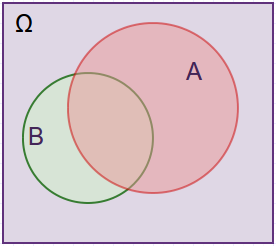
\includegraphics[scale=0.75]{img/Dvenn1.png}
\end{center}

\begin{defn}[Regla del producto]
Sean $\{A_1, A_2,...,A_n\}$ eventos con $P(A_i)>0$ entonces

\[
P(\bigcap_{i=1}^{\infty}A_i) = P(A_1)P(A_2|A_1)P(A_3|A_1\cap A_2)...P(A_n|A_1\cap A_2\cap ... \cap A_{n-1})
\]
(Suponiendo que $P(A_n|A_1\cap A_2\cap ... \cap A_{n-1})>0$)
\begin{proof}
\[
P(A_1)P(A_2|A_1)P(A_3|A_1\cap A_2)...P(A_n|A_1\cap A_2\cap ... \cap A_{n-1})=
\]
\[
=P(A_1)\frac{P(A_2\cap A_1)}{P(A_1)}\frac{P(A_3\cap A_2\cap A_1)}{P(A_2\cap A_1)}...\frac{P(\bigcap_{i=1}^{n-1}A_i)}{P(\bigcap_{i=1}^{n-2}A_i)}\frac{P(\bigcap_{i=1}^{n}A_i)}{P(\bigcap_{i=1}^{n-1}A_i)} = P(\bigcap_{i=1}^{n}A_i)
\]
\end{proof}
\end{defn}
\begin{example}
Caja con 10 bolas blancas y 10 bolas negras. Se extrae 1 bola y sin devolverla a la caja se extra otra segunda. ¿Cuál es la probabiidad de que las dos sean blancas?

P(2 blancas)=$\frac{10}{20}\frac{9}{19}$
\end{example}

\begin{defn}[Regla de la probabilidad total]
Sea  $\{A_1, A_2,...,A_n\}$ una partición de $\Omega$ con $P(A_i)>0 \forall i=1,2,...,n$. Entonces, $\forall B \subset \Omega$ medible (perteneciente a $\algb{M}$):
\[
P(B)=\sum_{i=1}^{n}P(B\cap A_i)=\sum_{i=1}^{n}P(B|A_i)P(A_i)
\]
(Se obtiene de despejar de la formula de la probabilidad condicionada: $P(A|B)=\frac{P(A \cap B)}{P(B)}$)
\end{defn}

\begin{figure}[h]
\centering
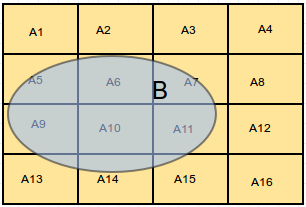
\includegraphics[page=1,scale=0.745]{img/Dvenn2.png}
\caption{Ejemplo de partición con n=16}
\end{figure}

\begin{defn}[Teorema de Bayes]
Modeliza la noción de "causa-efecto", donde $A_1, A_2,...,A_n$ son posibles causas del efecto B:
\[
P(A_i|B)= \frac{P(A_i\cap B)}{P(B)}= \frac{P(B|A_i)P(A_i)}{\sum_{k=1}^{n}P(B|A_k)P(A_k)}
\]

(Combina la regla de la probabilidad condicionada con la regla de la probabilidad total)
\end{defn}

\begin{defn}[Independencia]
\[
A,B \text{ son independientes} \Leftrightarrow P(A \cap B)=P(A)P(B)
\]

\obs Si un suceso A es independiente de otro suceso B (de modo que B no proporciona información útil sobre A) entonces $P(A|B)=P(A)$.
\obs Dada una sucesión finita $\{A_i\}_{i=1}^{n}$ o infinita $\{A_i\}_{i=1}^\infty$ de eventos, decimos que estos son independientes si toda subsucesión $A_{i_1}, A_{i_2},..., A_{i_n}$ con $(2 \leq n < \infty)$ finita, saisface:
\[
P(\bigcap_{i=1}^nA_{i_j})=\prod_{i=1}^{n}(P(A_{i_j}))
\]

\obs Los conjuntos $A_1, A_2,...,A_n$ son independientes 2 a 2 si $\forall$ par \{i,j\} con $i \neq j$, tenemos que $A_i$ y $A_j$ son independientes.

\begin{example}
Supongamos que A es independiente de A. Entonces tenemos que: $P(A\cap A)=P(A)=P(A)P(A) \Leftrightarrow P(A)=0$ ó $P(A)=1$
\end{example}
\end{defn}



\begin{example}
Sean A,B,C $\subset [0,1]$ con los borelianos (la $\salgb$ generada por los abiertos) y la medida de Lebesgue $\lambda$. Observamos que este espacio de medida coincide con un espacio de probabilidad con función de probabilidad uniforme P.

Es decir, tenemos 3 conjuntos que son uniones numerables o complementarios de intervalos en $[0,1]$. Estos conjuntos no son independientes. Vamos a definir una nueva probabilidad de manera que tengamos independencia con conjuntos semejantes a estos:

\~{A} $= A\times[0,1]^2 \subset [0,1]^3$

\~{B} $= [0,1]\times B \times[0,1]$

\~{C} $= C \times[0,1]^2$

Por tanto \~{A}, \~{B} y \~{C} son independientes y \~{A} $\cap$ \~{B} = $\{x \in [0,1]^3, x=(x_1, x_2, x_3) | x_1 \in A, x_2 \in B, x_3 \in [0,1]\}$.

Y podemos definir \~{P}(\~{A}$\cap$ \~{B})=$P(A)P(B)P([0,1])$ (por definición de medida producto)

Siendo \~{P} en $[0,1]^3$ la probabilidad producto.

Además \~{P}(\~{A}$\cap$\~{C}) = \~{P}(\~{A})\~{P}(\~{C})=$P(A)P(C)$ etcetera etcetera...

Unos dibujitos aclaratorios, para hacerlo más fácil consideramos que estamos en $[0,1]^2$ y:

$A1 = A\times[0,1]$

$B1 = [0,1]\times B$

\begin{figure}[h]
\centering
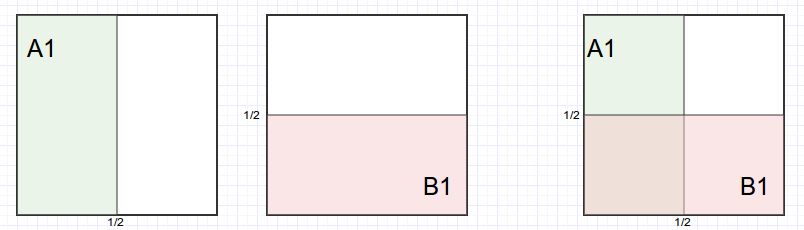
\includegraphics[page=1,scale=0.545]{img/Dvenn3.png}
\caption{A = [0,1/2], B=[0,1/2]}
\end{figure}

\end{example}

\begin{defn}[Independencia de conjuntos respecto a otro conjunto] Sea $P(C)>0 \Rightarrow$ A y B son condicionalmente independientes con respecto a C si:
\[
P(A\cap B|C)=P(A|C)P(B|C)
\]

Es decir, A y B son independientes entre ellos tomando como $\Omega$ el conjunto C.

Entonces si $P(B\cap C)>0$, se cumple que $P(A|B\cap C)=P(A|C)$
\end{defn}

\begin{defn} [Variable aleatoria]
Dado ($\Omega_1$,$\algb{M}$) y ($\Omega_2$,$\algb{B}$):
\[
X: \Omega_1 \rightarrow \Omega_2 \text{es una variable aleatoria} \Leftrightarrow \forall B \in \algb{B}, X^{-1}(B) \in \algb{M}
\]

En este curso usaremos como $\Omega_2$ conjuntos como $\mathbb{R}$ o $\mathbb{R} \cup \{\pm \infty\}$ o $\mathbb{C}$. Si $\Omega_2 = \mathbb{R}^d$, decimos que la función medible $X: \Omega_1 \rightarrow \mathbb{R}^d$ es un vector medible.
\end{defn}
\obs \textbf{IMPORTANTE. }Una variable aleatoria es una función medible.

\begin{defn}[Variable aleatoria discreta]
Una variable aleatoria X es discreta $\Leftrightarrow$ $P_X$ es discreta. Es decir, si toma valores en un conjunto numerable. Se caracteriza por tener una función de masa o de probabilidad, y una función de distribución.

Otras definiciones:

Recordemos que X es una función. $X: \Omega \rightarrow \mathbb{R}$. X es discreta si existe un conjunto numerable $x_1, x_2,...,x_n \in \mathbb{R}$ (siendo $x_i=X(w_i)$) tal que $P(\bigcup_{i=1}^{\infty}x_i=1)$.

$P_X$ es discreta si $P_X(\mathbb{R})=\sum_{i=1}^{\infty}P(X=x_i)$ (es decir, se puede expresar como un sumatorio numerable).
\end{defn}

\begin{defn}[Variable aleatoria continua]
Una variable aleatoria es continua si toma valores en un conjunto no numerable. Tiene asociada una función de densidad o de probabilidad, y una función de distribución.

X es una variable aleatoria continua $\Leftrightarrow$ $P_x$ es absolutamente continua con respecto a la medida de Lebesgue ($\lambda$) (se escribe $P_X << \lambda$) $\Leftrightarrow F_X$ es una función absolutamente continua $\Leftrightarrow$ $f_X=F_X'$ satisface que $F_X(t)=\int_{-\infty}^{t}f_X(x)dx$.
\end{defn}

\begin{defn}[Función de distribución]
\[
F_X(t)=P(X^{-1}(-\infty,t])=P_X(X \leq t)
\]

Así tenemos que: $P_X((a,b])=F_X(b)-F_X(a)$

La función de distribución cumple:
\begin{itemize}
\item $\lim_{n \rightarrow \infty}F(x)=1$
\item $\lim_{n \rightarrow -\infty}F(x)=0$
\item $F(t)=\int_{-\infty}^{t}f(x)dx$
\end{itemize}

\end{defn}

\begin{defn}[ley de X]
Dado el espacio de probabilidad ($\Omega, \algb{M}, P$) y la variable aleatoria $X: \Omega \rightarrow \mathbb{R}$, la ley de X es la probabilidad en $\mathbb{R}$ definida mediante:
\[
P_x(B)=P(X^{-1}(B)) \text{ } \forall B \in Borel(\mathbb{R})
\]

Notación: $P_x(B) = P(X^{-1}(B)) = P(\{w \in \Omega : X(w) \in B\})=P(X \in B)$

Notación: $Borel(\mathbb{R})$ es el conjunto de intervalos en $\mathbb{R}$, (los borelianos de toda la vida).


\end{defn}


\begin{example}

\textbf{ PARA ACLARAR LO QUE ES UNA FUNCIÓN MEDIBLE }Supongamos un dado de 6 caras. Tomamos dos situaciones:
\begin{enumerate}
\item  $\Omega = \{1,2,3,4,5,6\}$ y $\algb{M}=\mathbb{P}(\Omega)$.

Entonces la función X se define:

$X: \Omega \rightarrow \mathbb{R}$

Todas las funciones X son medibles ya que tenemos $(\Omega,\algb{M})$ y $(\mathbb{R}, Borel(\mathbb{R}))$, y entonces $\forall A \in Borel(\mathbb{R})$ tenemos que $X^{-1}(Borel(\mathbb{R})) \in \algb{M}$

Una vez definidos cuales son los medibles en los conjuntos de salida $(\Omega,\algb{M})$ y de llegada $(\mathbb{R}, Borel(\mathbb{R}))$. Podemos definir la siguiente variable aleatoria X.

$X(w) = 1$ si $w=3$

$X(w) = 0$ si $w\neq3$

Siendo $w \in \Omega$, esta variable aleatoria es equivalente a $X(w) = \ind_{\{3\}}$.

De esta manera podemos ver que: $X^{-1}(\{1\}) = \{3\}$, $X^{-1}(\{0\}) = \{1,2,4,5,6\}$, $X^{-1}((1/2,\infty)) = \{3\}$, y $X^{-1}((-2,\infty)) = \Omega$ entre otros ejemplos.


\item $\Omega = \{1,2,3,4,5,6\}$ y $\algb{B} = \{\Omega, \emptyset, \{1,3,5\}, \{2,4,6\} \}$

Entonces la función X se define:

$X: \Omega \rightarrow \mathbb{R}$

Pero en este caso, las funciones medibles ($\algb{B}-medibles$) son aquellas que son constantes en $\{1,3,5\}$ y en $\{2,4,6\}$. Ya que por ejemplo si tengo una función del tipo: $X(\{1\})=1$, $X(\{2\})=2$, $X(\{3\})=3$, $X(\{4\})=4$, $X(\{5\})=5$, $X(\{6\})=6$. Y calculo $X^{-1}((1/2, 3/2))=\{1\}$, que no pertenece a $\algb{B}$ y no es medible, por tanto X no sería medible y no sería una variable aleatoria.
\end{enumerate}

\obs Dada una función $X:(\Omega, \algb{M}) \rightarrow (\mathbb{R}, Borel(\mathbb{R}))$, para comprobar que es una función medible, y por tanto que es una variable aleatoria (es decir, que $\forall B \in Borel(\mathbb{R}) \rightarrow X^{-1}(B) \in \algb{M}$), basta comprobarlo para cualquier clase que genere a los borelianos (a $Borel(\mathbb{R})$).

Puesto que $Borel(\mathbb{R})=\{(r,\infty): r\in \mathbb{Q}\}$, para ver que X es una variable aleatoria basta comprobar que $\forall r \in \mathbb{Q}, X^{-1}((r, \infty)) \in \algb{M}$.

\end{example}

\begin{defn}[Esperanza o media]
Sea un espacio de probabilidad $\{\Omega, \algb{M},P\}$, la media o esperanza de una variable aleatoria X es:
\[
E(X)=E_p(X)=\int_{\Omega}X(w)dP(w)
\]

Si la variable aleatoria es continua:

\[
E(X)=E_p(X)=\int_{\Omega}X(w)dP(w) = \int_{-\infty}^{\infty}x\cdot dP_X(x)= \int_{-\infty}^{\infty}x\cdot dF_X(x) = \int_{-\infty}^{\infty}x\cdot f_P(x) dx
\]

Donde $F_X(t)=P(X \leq t)$ es la función de distribución de X y $f(t)=F'_X(t)$ la de densidad.

Si es discreta:

\[
E(X)=\sum_{n=1}^{\infty}X(w_n)P(w_n)
\]


\obs \textbf{Breve explicación del concepto de integrar respecto a una medida}(Desde aquí hasta la definición de varianza hay una explicación, posiblemente obvia para muchos lectores,  de lo que es derivar con respecto a una medida, además esta escrita con mis palabras con lo que puede que os liéis, si es así, os recomiendo borrarla de la cabeza, aunque también puede servir) Derivar con respecto a P(w), es derivar con respecto a una medida, que tal y como hemos visto en TIM es equivalente a derivar la función de distribución de dicha medida e integrar con respecto a x. O lo que es lo mismo, multiplicar por la función de densidad.

El concepto es natural en este caso, si se piensa que la integral es una suma infinita, y si derivas con respecto a una medida lo que quieres es obtener la medida de cada $w \in \Omega$. En este caso se suele hacer un cambio de variable, e integrar en $\mathbb{R}$ en lugar de en $\Omega$, por tanto ahora integras las x=X(w), y pones la función de densidad, que asigna a cada valor X(w) su probabilidad (sabemos que al hacer la integral estamos considerando que la variable aleatoria es continua, y no discreta, y que por tanto la probabilidad de un evento es igual a la probabilidad de un punto, que es 0 ya que el area bajo un punto es 0), que es lo equivalente a la función de probabilidad, de manera que queda:

\[
E(X)=E_p(X)=\int_{\Omega}X(w)dP(w) = \int_{\mathbb{R}}x\cdot dP_X(x)= \int_{\mathbb{R}}x\cdot dF(x) = \int_{\mathbb{R}}x\cdot f(x) dx
\]

Siendo $f(x)$ la función de densidad asociada a esa probabilidad (a esa función de distribución P), que aplicando el Tma. Fundamental del Calculo (ver capitulo 1):

\[
F(x) = \int_{-\infty}^{x}f(x)dx  \rightarrow \frac{dF(x)}{dx}= f(x) \rightarrow dF(x) = f(x)dx
\]

Por tanto, dada una integral con respecto a una medida $\mu$, primero obtenemos la función de distribución asociada a $\mu$ y posteriormente derivamos esa función de distribución obteniendo la función de densidad y la integral con respecto a x, que sí sabemos resolver.

Cuando la variable aleatoria es discreta la esperanza se calculará como una suma finita por la medida (probabilidad) de cada evento $w \in \Omega$.

%\obs $P(a \leq w \leq b)= \int_{b}^{a} f(x)dx$, por tanto: $dP(a \leq w \leq b) = f(b)-f(a).
\end{defn}


\begin{defn}[Varianza]
Sea un espacio de probabilidad $\{\Omega, \algb{M},P\}$, la varianza de una una variable aleatoria X es:
\[
var(X)=E[(X-E(X))^2] = E(X^2)-E(X)^2
\]

\obs Si $X(w)=c$  $\forall w$, entonces $E(X)=c$
\obs E(E(X))=E(X)
\end{defn}

\begin{defn}[Formula del cambio de variable]
Sea $X: \Omega \rightarrow \mathbb{R}$ una variable aleatoria, y sea $g:\mathbb{R} \rightarrow \mathbb{R}$ una función de Borel. Entonces:

\[
\mathbb{E}(g(X))=\int_{\Omega}g(X(w))dP(w)=\int_{\mathbb{R}}g(x)dP_X(x)
\]

Recordatorio: $P_X(A)=P(X\in A)=P(X^{-1}(A))$
\end{defn}


\begin{proof}
\textbf{De la fórmula del cambio de variable} Esta demostración puede servir para aclarar algunos conceptos de TIM, lo hacemos despacio:

\begin{enumerate}
\item Primero vamos a ver que es cierto para funciones $g=\ind_{B}$, con $B \in Borel(\mathbb{R})$. De manera que por ser una función indicatriz se cumple que: $\ind_{B}(X(w))=1 \Leftrightarrow X(w) \in B$.

En este caso tendríamos (Usamos la definición de integrar respecto a una medida una función indicatriz):
\[
\mathbb{E}(g(X(w))) = \mathbb{E}(g(X)) = \mathbb{E}(\ind_{B}(X))=\int_{\Omega}\ind_{B}(X(w))dP(w) =
\]
\[
= P(X(w)\in B) = P(X^{-1}(B))=P_X(B)=\int_{\Omega}\ind_{B}(x)dP_X(x)
\]

Breve explicación:
\begin{itemize}
\item Poner o no la 'w' al poner X(w) no es más que notación, se sobreentiende que esa w siempre esta ahí, ya que X es una variable aleatoria, y por tanto una función que depende de w.
\item Estamos integrando sobre un espacio $\Omega$, sin embargo la indicatriz esta evaluada sobre un espacio de Borel que no tiene por que pertenecer a $\Omega$. Por eso, el resultado de la integral no es P(B) que es lo que sería aplicando la definición anterior (si ocurriera que $B\in \Omega$). En este caso, el resultado sera la medida P de todos los $w \in \Omega$ que provocan que $X(w) \in B$.
\item La última igualdad sale por definición de integrar respecto a una medida una función indicatriz.
\end{itemize}
\item Si $g \geq 0$ (es decir, $g \in L^+$), entonces, por el teorema de la aproximación de funciones simples, existe una sucesión $s_n\nearrow g$ (converge a g en todo punto y la sucesión es monótona creciente). Así podemos escribir:

\[
\int g dP = \int \lim_{n \rightarrow \infty}s_n dP \stackrel{TCM}{=} \lim_{n \rightarrow \infty}\int s_n dP
\]

Y dicha integral la sabemos resolver aplicando la definición de integral sobre funciones simples que hemos visto anteriormente y aplicando el punto 1 de esta demostración.
\item Y el último caso sería una funcion $g:\mathbb{R} \rightarrow \mathbb{R}$, en cuyo caso escribimos $g=g_+-g_-$ (ver capitulo 1.3). Y nos queda $\int gdP = \int g_+dP -\int g_-dP$(por la linealidad de la integral).

Por tanto hemos expresado g como resta de dos funciones $g_+$ y $g_-$, ambas pertenecientes a $L^+$. Entonces podemos hallar $\int g$ aplicando el punto 2 de esta demostración. Debemos tener en cuenta que $\int g$ existirá si: $\int g_+dP < \infty$ ó $\int g_-dP < \infty$

\end{enumerate}
\end{proof}


\begin{example}
\begin{itemize}
\item $\mathbb{E}(X)$ no esá bien definida si $\int_{\mathbb{R}}X_+ dP_X=\infty$ y $\int_{\mathbb{R}}X_- dP_X=\infty$.

\item $\mathbb{E}(X^2)$ siempre esta bien definida ya que $(X^2)_-=0$.
\item Si $X \geq 0$, $\mathbb{E}(X)$ está bien definida.
\item Sea una variable aleatoria de Bernoulli de parámetro p. Entonces $P(X=1)=p$ y $P(X=0)=1-p$. Llamamos función de masa a $P(X=i)$.

$\mathbb{E}(X)$ está bien definida porque X(w) es siempre $\geq 0$.

\[
\mathbb{E}(X)=0\cdot P(X=0)+1\cdot P(X=1)=0\cdot(1-p)+1\cdot p=p
\]
\[
\mathbb{E}(X^2)=0^2\cdot P(X=0)+1^2\cdot P(X=1)=0^2\cdot(1-p)+1^2\cdot p=p
\]
\[
\mathbb{V}(X)=\mathbb{E}(X^2)-\mathbb{E}(X)^2=p-p^2=p(1-p)
\]
\item Sea $S_n=X_1+X_2+...+X_n$, con $X_i=Bernoulli(p)$, entonces $S_n \sim Binomial=B(n,p)$.
\[
\mathbb{E}(S_n)=\mathbb{E}(\sum_{i=1}^{n}X_i)\stackrel{linealidad integral}{=}\sum_{i=1}^{n}(\mathbb{E}(X_i))=np
\]
\item $X\sim N(0,1)$
Sabemos que $f_X(x)=\frac{e^{-x^2/2}}{\sqrt{2\pi}}$, por tanto:

\[
\mathbb{E}(g(X))=\int_{-\infty}^{\infty}g(x)\frac{e^{-x^2/2}}{\sqrt{2\pi}}dx
\]
\end{itemize}
\end{example}

\chapter{Esperanza condicionada (Tema 1)}

Empezamos definiendo una serie de conceptos que usaremos más adelante:

\begin{defn}[Norma y convergencia]
Sea $(X, \algb{M}, \mu)$ un espacio de medida. Para $0<p<\infty$, definimos $L^p=L^p(X,\algb{M},\mu)=\{f:X\rightarrow \mathbb{R}$ ó $\mathbb{C} | \int_X \abs{f}^p d\mu < \infty\}$

\begin{itemize}
\item Si $p \geq 1$, entonces $\norm{f}_p = (\int_X {\abs{f}^p d\mu)}^{\frac{1}{p}}$ es una norma. Algo es una si cumple estas tres propiedades:
\begin{enumerate}
\item Positividad: $\norm{f}\geq 0$ y $\norm{f} = 0 \Leftrightarrow f=0$.
\item Proporcionalidad: $\norm{\lambda f} = \abs{\lambda}\norm{f}$.
\item Desigualdad triangular: $\norm{u+v} \leq \norm{u}+\norm{v}$
\end{enumerate}
\item Y decimos que una función converge en $L_p$:

\[
f_n \stackrel{L_p (n\rightarrow \infty)}{\rightarrow} g \Leftrightarrow \norm{f_n -g}_p  \rightarrow 0 \Leftrightarrow \int{\abs{f_n -g}^pd\mu} \rightarrow 0
\]
\end{itemize}

\obs En los ejercicios se toma como $\mu$ la probabilidad P, y como X, se toma $\Omega$, de al manera que estás integrando sobre un espacio que mide como mucho 1. Lo que significa que por ejemplo sea f=1, entonces: $\int_{\Omega}fdP = 1$, mientras que $\int_{\mathbb{R}}fdx = \infty$

\obs Definimos la norma infinito de f como el supremo esencial de f. (En otras palabras, el valor máximo del valor absoluto de f)


\end{defn}

\begin{defn}[medida absolutamente continua con respecto a otra $\mu << \nu$]
$\mu << \nu$ si $\mu(A)=0 \Rightarrow \nu(A)=0$

\begin{example}
Sea $f \geq 0$ medible y sea $\mu(A)=0$, entonces $\int_Afd\mu=0$ (se ve fácil con la fórmula del cambio de variable). Si defino $\nu(B)=\int_B fd\mu$, entonces tenemos que $\mu << \nu$.
\end{example}
\end{defn}

\begin{defn}[medida con signo]
Sea $f:\mathbb{R}\rightarrow \mathbb{R}$, entonces $\nu(B)=\int_B fd\nu$ es una medida con signo (y además $\mu << \nu$). Es una medida con signo ya que al ser una medida que depende de una función que va de $[-\infty, \infty]$, puede adquirir valores negativos.
\end{defn}

\begin{defn}
X es una variable aleatoria continua $\Leftrightarrow$ $P_x$ es absolutamente continua con respecto a la medida de Lebesgue ($\lambda$) (se escribe $P_X << \lambda$)
\end{defn}

\begin{theorem}[Teorema de Radon-Nikodyn]
Sea $\nu << \mu$ una medida con signo ($\mu \geq 0$, $\mu$ y $\nu$ son $\sfin$, y $\nu_+(X) < \infty$ ó $\nu_-(X) < \infty$). Entonces existe una funcion f medible tal que $f:X \rightarrow \mathbb{R}$ que cumple que $\forall B$ medible $\subset X$ se cumple $\nu(B)=\int_Bfd\mu$. Escribimos $f=\frac{d\nu}{d\mu}$, la derivada de Radon-Nikodyn.
\end{theorem}


\begin{defn}[sigma-álgebra generada por una función]
Sea $Y: \Omega \rightarrow \mathbb{R}$, entonces $\sigma(Y)$ es la $\salgb$ más pequeña que hace que Y sea medible, es decir: $\{Y^{-1}(B):B \in Borel(\mathbb{R})\}$
\end{defn}

\obs También podemos escribir $\sigma(Z)$ siendo Z un conjunto de elementos (por ejemplo una parición) de $\Omega$. Y se referirá a la $\salgb$ generada por ese conjunto de elementos.

\begin{example}
Sea una función $Y:\mathbb{R} \rightarrow \mathbb{R}$ definida mediante $Y=\ind_{[0,\infty]}$, entonces $\sigma(Y)=\{\emptyset, (-\infty, 0), [0, \infty), \Omega \}$.

\begin{expla}
Y es una función que vale 0 en el intervalo $(-\infty, 0)$ y 1 en el intervalo $[0, \infty)$, por tanto para que Y sea medible (sea una variable aleatoria) tiene que cumplir que la imagen de los elementos pertenecientes al conjunto de salida ($\mathbb{R}$), sean constantes en el de llegada ($\mathbb{R}$). Como el conjunto de llegada consta de dos intervalos constantes ( vale 0 en el intervalo $(-\infty, 0)$ y 1 en el intervalo $[0, \infty)$); concluimos que la mínima $\salgb$ generada por la función Y es $\sigma(Y)=\{\emptyset, (-\infty, 0), [0, \infty), \Omega \}$.
\end{expla}

\end{example}

\begin{defn}[Esperanza condicionada]

Sabemos que si $P(B)>0$, entonces definimos $P_B(A)=\frac{P(A \cap B)}{P(B)}=P(A|B)$

Entonces definimos la esperanza condicionada como:

\[
E_{P_B}(X)=\frac{1}{P(B)}\int_{B}X(w)dP(w)=E(X|B)
\]
\end{defn}

\obs También se escribe $\mathbb{E}(X|Y)$ siendo Y una variable aleatoria. Además $\mathbb{E}(X|Y)$ = $\mathbb{E}(X|\sigma(Y))$ (es sólo notación, queremos decir lo mismo de las dos maneras)


\begin{defn}[Esperanza condicionada (como función de una sub-$\salgb$)]
Dado el espacio de probabilidad $(\Omega, \algb{M}, P)$ y la sub-$\salgb$ $\mathbb{B}\subset\algb{M}$ generada a partir de una partición de $\Omega$ (más adelante veremos que no es necesario que esté generada por una partición, sino que valdrá cualquier  sub-$\salgb$), la esperanza condicionada $\mathbb{E}(X|\algb{B})$ es:
\begin{enumerate}
\item $\algb{B}$-medible
\item $\forall B \in \algb{B}$, $\int_{B}\mathbb{E}(X|\algb{B})dP=\int_{B}XdP$

Estas dos propiedades determinan $\mathbb{E}(X|\algb{B})$ de modo único.
\end{enumerate}
\end{defn}

\obs Cuando definimos $\mathbb{E}(X|\algb{B})$, esto es una función evaluada en $w \in \Omega$.

\obs Sea $\algb{B}=\sigma(\{A_i\}_{i=1}^{\infty})$, siendo $\{A_i\}_{i=1}^{\infty}$ una partición de $\Omega$ con $P(A_i)>0$. Entonces:
\[
\mathbb{E}(X|\algb{B})(w)=\sum_{i=1}^{\infty}\left( \frac{1}{P(A_i)}\int X(w)dP(w)\right)\ind_{A_i(w)}=\sum_{i=1}^{\infty}\mathbb{E}(X|A_i) \ind_{A_i}
\]

\obs $\norm{Y}_p^p = \mathbb{E}(\abs{Y}^p)$
\begin{proof}
\[
\norm{Y}_p = \int \abs{Y}^pdP =\mathbb{E}(\abs{Y}^p)
\]
\end{proof}



\begin{example}
Sea X e Y variables aleatorias. Dado $(\Omega, \algb{M}, P)$, siendo $\Omega$ la población de un lugar, y siendo $\algb{M}$ una $\salgb$.

X = estatura de una población, tal que $X(w)=x \forall w \in \Omega$

Y = sexo de esa misma población, tal que $Y(w)=1$ si w es mujer, e $Y(w)=0$ si w es hombre.

Definimos la sub-$\salgb$ $\algb{B}=\{\emptyset, \Omega, \{Y=1\}, \{Y=0\}\}$, de manera que $\algb{B} \subset \algb{M}$, y por tanto contiene menos información.
\end{example}

De esta manera, hemos visto que es posible definir la esperanza condicionada ($\mathbb{E}(X|\algb(B))$) cuando $\algb(B)$ esta generada por una partición de $\Omega$. Sin embargo no toda sub-$\salgb$ va a estar generada por una partición. Por ejemplo $Borel(0,1)$ no esta generado por ninguna partición.

Por tanto vamos a definir la esperanza condicionada de otra forma:

\section{Esperanza condicionada como proyección ortogonal en $L^2$}
Recordemos que:

Sea $(\Omega, \algb{M}, \mu)$ un espacio de medida. Para $0<p<\infty$, definimos $L^p=L^p(\Omega,\algb{M},\mu)=\{f:\Omega\rightarrow \mathbb{R}$ ó $\mathbb{C} | \int_X \abs{f}^p d\mu < \infty\}$

En otras palabras:
$$
\text{si } 0<p<\infty =
  \left\lbrace
  \begin{array}{l}
     f\in L^p(\Omega,\algb{M},\mu) \Leftrightarrow \int \abs{f}^p < \infty \\
     f\in L^{\infty}(\Omega,\algb{M},\mu) \Leftrightarrow \text{supremo esencial } \abs{f} < \infty) \\
  \end{array}
  \right.
$$

El supremo esencial de una función f es:

$supEsencial(f)=sup\{c\geq0:\mu\{\abs{f}\geq c\}>0\}$

Es decir, el valor mayor de f. Por ejemplo, si $f=\frac{1}{x}$ en el intervalo (0,1), $supEsencial(f)=\infty$.

Vamos a definir $\mathbb{E}(X|\algb{B})$ para $X\in  L^2(\Omega,\algb{M},P)$. Utilizamos $L^2$ ya que es un espacio vectorial normado con norma $\norm{X}_2 = (\int_\Omega {X^2 dP})^{\frac{1}{p}}$, y producto escalar que cumple:

$<X,Y> = \int_{\Omega}XYdP$

$\norm{X}=(<X,X>)^{\frac{1}{2}}$

Resumiendo, queremos definir la esperanza condicionada ($\mathbb{E}(X|\algb{B})$), y para ello hemos definido un espacio vectorial $L^2(\Omega,\algb{M},P)$, que esta formado por vectores (las variables aleaorias), por una operación interna (la suma) y por una externa (el producto escalar):
\begin{itemize}
\item Vectores: las variables aleatorias X conformarán los elementos de nuestro espacio vectorial.
\item Producto escalar: $<X,Y> = \int_{\Omega}XYdP$
\end{itemize}

De esto se deduce la norma de un vector, que será: $\norm{X}=(<X,X>)^{\frac{1}{2}}$

Ahora vamos a comprobar que podemos extender la definición a $L^1$, ya que $L^2(P) \subset L^1(P)$. Lo demostramos:

\begin{proof}
Si $f \in L^2(P) \Rightarrow \int f^2 < \infty$.

Escribimos:
\[
\int \abs{f} = \int \abs{f}\ind_{\{\abs{f}\leq 1\}} + \int \abs{f}\ind_{\{\abs{f}> 1\}}
\]

El primer sumando es menor o igual que 1 ya que estamos integrando una función sobre $\Omega$ y con respecto a P, y P es una medida de probabilidad, que asigna a cada valor un número entre 0 y 1. Por tanto, sabiendo $\int_{\Omega}dP = 1$ (por definición de integral con respecto a una medida y sabiendo que P es una función de probabilidad y que $P(\Omega)=1$), si cogemos los valores de f, que son menores que 1, nos dará un numero menor o igual que 1, que multiplica como mucho a 1:
\[
\int_{\Omega} \abs{f}\ind_{\{\abs{f}\leq 1\}}dP \leq 1
\]

Y el segundo sumando se ve claro que es menor que infinito ya que:
\[
 \int_{\Omega} \abs{f}\ind_{\{\abs{f}> 1\}}dP \leq  \int_{\Omega} f^2 dP < \infty
\]

Por tanto nos queda que:
\[
\int \abs{f} < \infty
\]

Que es precisamente lo que significa que $f\in L^1$
\end{proof}

%\textcolor{red}{Extender el resultado a $L^1$ lo hacemos por que??¿?¿?¿?¿¿, por que así nos basta con funciones $L^1$.}

A partir de ahora nos referiremos con $L^2(\algb{M})$ a $L^2(\Omega,\algb{M},P)$.
Si a partir de ahora empieza a resultar lioso, lo intento explicar con un dibujillo y tal al final.

Ahora vamos a definir la sub-$\salgb$ $\algb{B} \subset \algb{M}$, la cual va a formar un subespacio vectorial $L^2(\Omega,\algb{B},P) \subset L^2(\Omega,\algb{M},P)$. Este subespacio vectorial es cerrado, es decir, una sucesión de elementos dentro del subespacio converge a un elemento dentro del subespacio:
\[
\text{Si} g_n \in L^2(\algb{B}) y \lim_{n \rightarrow \infty} \norm{g_n -f}_2 = 0 \Rightarrow f \in L^2(\algb{B})
\]

Definimos ahora la proyección ortogonal de un elemento de $L^2(\algb{M})$ en otro de $L^2(\algb{B})$.
\[
T: L^2(\algb{M}) \rightarrow L^2(\algb{B})
\]
Por tanto, si $X\in L^2(\algb{M})$, tenemos que $X-T(X) \perp L^2(\algb{B})$, o lo que es lo mismo, si $Y \in L^2(\algb{B})$, entonces $<X-T(X),Y>=\int(X-T(X))Y = 0$.

Una vez hemos definido bien T como la proyección ortogonal de un elemento (una variable aleatoria X) del espacio de vectorial $L^2(\algb{M})$ al subespacio vectorial $L^2(\algb{B})$, ahora vamos a demostrar que T es la esperanza condicionada de X con respecto de $\algb{B}$.

Para ello debe cumplir las dos propiedades:
\begin{enumerate}
\item T(X) es $\algb{B}$-medible. Es obvio ya que $T(X) \in L^2(\algb{B})$

\item $\int_B X =\int_B T(X)$  $\forall B \in \algb{B}$

Lo demostramos usando la ortogonalidad: Escogemos un elemento $B \in \algb{B}$, entonces $\ind_{\algb{B}} \in L^2(\algb{B})$. Esto es obvio ya que:
\[
\norm{\ind_B}_2=(\int_{\Omega}\ind_B^2)^{\frac{1}{2}}=\sqrt{P(B)}<\infty
\]

Y por tanto tenemos que:
\[
0=<X-T(X),\ind_B> = \int_{\Omega}(X-T(X))\ind_B dP= \int_B(X-T(X)) dP= \int_B X dP - \int_B T(X) dP \Rightarrow
\]
\[
\Rightarrow \int_B X dP = \int_B T(X) dP
\]
\end{enumerate}

Vemos que T(X) cumple las condiciones que debe cumplir una función para ser considerada esperanza condicionada. Por tanto, la proyección ortogonal de $L^2(\algb{M})$ en $L^2(\algb{B})$ es $\mathbb{E}(X|\algb{B})$ $\forall X \in \algb{M}$.

Y lo que es más importante, esto se cumple para toda sub-$\salgb$ de $\algb{M}$ y no solo para aquellas que están generadas a partir de una partición.

Además, $\mathbb{E}(X|\algb{B})$ es lineal en $L^2(\algb{M})$ y se cumple que:
\[
\mathbb{E}(aX+Y|\algb{B})=a\cdot\mathbb{E}(X|\algb{B})+\mathbb{E}(Y|\algb{B})
\]

El dibujito prometido, todo lo que se ve es ele spacio vectorial $L^2(\Omega,\algb{M},P)$. La recta azul es el subespacio vectorial $L^2(\Omega,\algb{B},P)$, que como todo subespacio vectorial debe contener al (0,0). Y la recta roja representa la proyección ortogonal de la variable aleatoria X sobre el subespacio vectorial $L^2(\Omega,\algb{B},P)$. Ahora sólo hay que trabajar con los vectores y el producto escalar que hemos definido.
\begin{figure}[h]
\centering
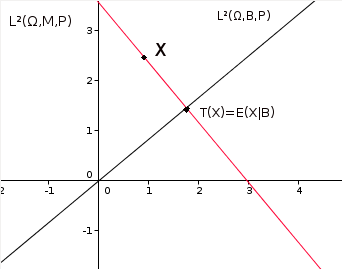
\includegraphics[page=1,scale=0.745]{img/graf1.png}
\end{figure}

\section{Esperanza condicionada usando el Teorema de Radon-Nikodyn}
Teorema de Radon-Nikodyn (caso especial): Sea $(\Omega, \algb{M})$ un espacio medible. Sea P una probabilidad en $\algb{M}$, y sea $\nu$ una medida con signo finita. Entonces, si $\nu<<P$, existe una función medible en $\frac{d\nu}{dP} \in L^1(\Omega, \algb{M}, P)$ tal que $\forall A \in \algb{M}$, $\nu(A)=\int \frac{
d\nu}{dP} dP$.

Así pues vamos a usar este teorema para probar la existencia de la esperanza condicionada ($\mathbb{E}(X|\algb{B})$) para $X \in L^1(\Omega, \algb{M}, P)$ aplicado a $L^1(\Omega, \algb{B}, P)$. Definimos $\nu$ en $\algb{B} \subset \algb{M}$ como $\nu(B)=\int_B XdP$

Recordemos que si $P(B)=0$, entonces $\nu(B)=0$. Que, en ese caso, esto ocurre si y solo si $\nu << P|_{\algb{B}}$. Por el teorema de Radon-Nikodyn existe $\frac{d\nu}{dP} \in L^1(\Omega, \algb{B}, P)$ tal que $\nu(B)=\int_B \frac{d\nu}{dP} dP$ para todo $B \in \algb{B}$. Luego $\mathbb{E}(X|\algb{B})=\frac{d\nu}{dP}$ es la derivada de Radon-Nikodyn y cumple:
\begin{enumerate}
\item es $\algb{B}$-medible.

\item $\int_B X dP =\nu(B) = \int_B \frac{d\nu}{dP} dP$  $\forall B \in \algb{B}$
\end{enumerate}


\section{Propiedades}
\begin{enumerate}
\item Linealidad: Si $\alpha$ es una constante $\in \mathbb{R}$ y $X,Y:\Omega \rightarrow \mathbb{R}$ con $X,Y \in L^1(\algb{M})$, entonces $\mathbb{E}(\alpha X + Y|\algb{B})=\alpha\mathbb{E}(X|\algb{B})+\mathbb{E}(Y|\algb{B})$

\begin{proof}
Ambos lados son $\algb{B}$-medibles (por definición de esperanza condicionada). Para demostrarlo vamos a utilizar la linealidad de la integral y la definición de esperanza condicionada(el punto 2: $\forall B \in \algb{B}$, $\int_{B}\mathbb{E}(X|\algb{B})dP=\int_{B}XdP$), entonces:
\[
\int_B \mathbb{E}(\alpha X + Y|\algb{B})dP= \int_B(\alpha X+Y)dP=\alpha\int_B XdP + \int_B YdP=
\]
\[
=\alpha\int_B \mathbb{E}(X|\algb{B})dP + \int_B \mathbb{E}(Y|\algb{B})dP = \int_B \left(\alpha\mathbb{E}(X|\algb{B}) + \mathbb{E}(Y|\algb{B})\right)dP
\]
\end{proof}
\item Positividad: Si $X \geq 0 \Rightarrow \mathbb{E}(X|\algb{B})\geq 0$. Equivalentemente si  $X \geq Y \Rightarrow \mathbb{E}(X|\algb{B})\geq \mathbb{E}(Y|\algb{B})$
\begin{proof}
Partimos de una variable aleatoria X que es positiva.

Sea $B=\{\mathbb{E}(X|\algb{B}) < 0\} \in \algb{B}$ (NOTACIÓN: son los w que cumplen eso)

Entonces:
\[
0 \geq  \int_B \mathbb{E}(X|\algb{B})dP = \int_B XdP \geq 0
\]

Y además tenemos que como $\mathbb{E}(X|\algb{B})<0$ en B, entonces $\int_B \mathbb{E}(X|\algb{B})dP=0$, lo que quiere decir que $P(B)=0$.
\end{proof}
\item $\abs{\mathbb{E}(X|\algb{B})} \leq \mathbb{E}(\abs{X}|\algb{B})$

\begin{proof}
Sabemos que podemos descomponer $X=X_+ - X_-$ y $\abs{X}=X_++X_-$, por tanto, aplicando la propiedad de la linealidad, la de $\abs{a-b} \leq |a|+|b|$ y la positividad de la esperanza nos queda que:
\[
\abs{\mathbb{E}(X|\algb{B})}=\abs{\left( \mathbb{E}(X_+|\algb{B}) - \mathbb{E}(X_-|\algb{B}) \right)} \leq \mathbb{E}(X_+|\algb{B})+\mathbb{E}(X_-|\algb{B})= \mathbb{E}(\abs{X}|\algb{B})
\]

\end{proof}
\item $\mathbb{E}(*|\algb{B})$ es una contracción en $L^1(\Omega, \algb{M},P)$, es decir, $\forall X \in L^1(\algb{M})$ se cumple que $\norm{\mathbb{E}(X|\algb{B})}_1 \leq \norm{X}_1$

\obs Como se cumple para $X \in L^1$, también se cumple para $X \in L^p$ , ya que $L^p \subset L^1$.

\obs Se demuestra que esto también se cumple para espacios $L^p$ (con la nueva definición de norma p) con $p>1$ más adelante.

\begin{proof}

Recordemos que $\norm{Y}_1 = \mathbb{E}(\abs{Y})$

Usamos la propiedad 3:
\[\norm{\mathbb{E}(X|\algb{B})}_1=
\mathbb{E}(\abs{\mathbb{E}(X|\algb{B})}) \leq \mathbb{E}(\mathbb{E}(\abs{X}|\algb{B})) = \mathbb{E}(\abs{X}) = \norm{X}_1
\]
\end{proof}
\item Teorema de la Convergencia Monótona(TCM) para $\mathbb{E}(X|\algb{B})$:
\[
\text{Si} 0\leq X_n \nearrow X \in L^1 \Rightarrow \lim_{n \rightarrow \infty} \mathbb{E}(X_n|\algb{B}) = \mathbb{E}(X|\algb{B})
\]
En casi todo punto y en $L^1$.

\begin{proof}
Vamos a usar el Teorema de la Convergencia Monótona (TCM) y el Teorema de la Convergencia Dominada (TCD) para integrales (ver anexo).

Sea $Y_n=X-X_n \geq 0$, usando la linealidad de la esperanza vemos que basta probar que $\lim_{n \rightarrow \infty} \mathbb{E}(Y_n|\algb{B})= \lim_{n \rightarrow \infty} \mathbb{E}(X-X_n|\algb{B}) = 0$ casi seguro y en $L^1$.

Por positividad (propiedad 2) tenemos que $Y_n \geq Y_{n+1} \Rightarrow \mathbb{E}(Y_n|\algb{B}) \geq \mathbb{E}(Y_{n+1}|\algb{B})$ luego el límite existe casi seguro porque van disminuyendo hasta 0 como mucho.

Así, sea $Z=\lim_{n \rightarrow \infty} \mathbb{E}(Y_n|\algb{B})$. Veamos que Z=0. Sea $B \in \algb{B}$, entonces:

\[
\int_B ZdP= \int_B \lim_{n \rightarrow \infty}\mathbb{E}(Y_n|\algb{B})dP= \lim_{n \rightarrow \infty}\int_B \mathbb{E}(Y_n|\algb{B})dP =
\]

El último paso es debido al TCD y a la propiedad 2 y 4. Usamos la propiedad 2 para ver que $0 \leq Y_n \leq X \Rightarrow 0 \leq \mathbb{E}(Y_n|\algb{B}) \leq \mathbb{E}(X|\algb{B})$.  Ahora usamos la propiedad 4 para ver que si $X\in L^1 \Rightarrow \mathbb{E}(X|\algb{B})\in L^1$ porque $\mathbb{E}(*|\algb{B})$ es una contracción. Por tanto podemos aplicar el TCD, ya que X nos hace la función de 'g' en dicho teorema.

Para el siguiente paso lo único que hacemos es aplicar la definición de esperanza condicionada (el punto 2: $\forall B \in \algb{B}$, $\int_{B}\mathbb{E}(X|\algb{B})dP=\int_{B}XdP$):

\[
\lim_{n \rightarrow \infty}\int_B Y_ndP \leq \lim_{n \rightarrow \infty}\int_{\Omega} Y_ndP =
\]

Y otra vez usamos el TCD:
\[
= \int_B \lim_{n \rightarrow \infty} Y_ndP = 0
\]

Ya que $0 \leq X_n \nearrow X$ y por tanto $Y_n = X-X_n \searrow 0 $. Y con esto lo hemos demostrado en casi todo punto.

Ahora vamos a ver que se cumple en $L^1$, es decir que:
\[
\lim_{n \rightarrow \infty} \mathbb{E}(X_n|\algb{B}) - \mathbb{E}(X|\algb{B}) = \lim_{n \rightarrow \infty} \mathbb{E}(X-X_n|\algb{B}) = 0 \text{ en } L^1
\]

Por tanto:
\[
 \lim_{n \rightarrow \infty} \norm{\mathbb{E}(X-X_n|\algb{B})}_1 = \lim_{n \rightarrow \infty} \norm{\mathbb{E}(X|\algb{B}) - \mathbb{E}(X_n|\algb{B})}_1 =
\]

\[
= \lim_{n \rightarrow \infty} \mathbb{E}\abs{\mathbb{E}(Y_n|\algb{B})} = \lim_{n \rightarrow \infty} \mathbb{E}(Y_n) \text{ y por el TCD = }  \mathbb{E}(\lim_{n \rightarrow \infty}Y_n)=0
\]
\end{proof}
\item Si X es $\algb{B}$-medible, entonces $\mathbb{E}(XY|\algb{B}) = X\mathbb{E}(Y|\algb{B})$, suponiendo que $XY,Y \in L^1$.

\obs Como esta definido para funciones en $L^1$, también funciona para funciones en $L^p$ para $p>1$, ya que $L^p \subset L^1$.
\begin{proof}
Empezamos suponiendo que $X=\ind_B$ con $B \in \algb{B}$. Entonces $\forall C \in \algb{B}$ se cumple que:
\[
\int_C \mathbb{E}(\ind_BY|\algb{B})dP = \int_C \ind_BYdP=\int_{C\cap B} YdP =
\]
\[
 =\int_{C\cap B} \mathbb{E}(Y|\algb{B})dP = \int_C \ind_B\mathbb{E}(Y|\algb{B})dP
\]

Luego:
\[
\mathbb{E}(\ind_BY|\algb{B}) = \ind_B\mathbb{E}(Y|\algb{B})
\]

Una vez demostrado para las X de esa forma es fácil demostrarlo para X de cualquier forma, sólo debemos ir aumentando poco a poco como en demostraciones anteriores.
\begin{itemize}
\item Si X es función simple, tenemos la misma igualdad por linealidad.
\item Si $X \geq 0$, escogemos $S_n$ sucesión de funciones $\algb{B}$-medibles con $S_n\geq 0$ y $S_n \nearrow X$ en casi todo punto (Teorema de aproximación de funciones medibles) y usamos la convergencia monótona.
\item Si X toma valores reales escribimos $X=X_+ - X_-$ y usamos linealidad de $\mathbb{E}(*|\algb{B})$.

\end{itemize}

\end{proof}
\obs Si X es $\algb{B}$-medible, entonces $\mathbb{E}(X|\algb{B})=X$
\begin{proof}
Tres maneras:
\begin{enumerate}
\item Teníamos que la esperanza condicionada ($\mathbb{E}(X|\algb{B})$) cumple que es $\algb{B}$-medible y que
$\forall B \in \algb{B}$, $\int_{B}\mathbb{E}(X|\algb{B})dP=\int_{B}XdP$, y ambas son $\algb{B}$-medibles, quiere decir que son constantes en los mismos conjuntos y además la integral en esos conjuntos vale lo mismo. Por lo tanto esa constante es la misma en las dos funciones.
\item Aplicando la propiedad 6 de las esperanzas condicionadas:
Si X es $\algb{B}$-medible, entonces $\mathbb{E}(XY|\algb{B}) = X\mathbb{E}(Y|\algb{B})$, suponiendo que $XY,Y \in L^1$.
\item Aplicando la definición de esperanza condicionada como proyección ortogonal. Antes dijimos que dada una sub-$\salgb$ $\algb{B} \subset \algb{M}$ un subespacio vectorial $L^1(\algb{B}) \subset L^1(\algb{B})$, entonces el punto más cercano de una variable aleatoria X en $L^1(\algb{M})$ (es decir, X es M-medible)a $L^1(\algb{B})$ (es decir, a una variable aleatoria que sea B-medible), es la proyección ortogonal de X sobre $L^1(\algb{B})$, y este punto coincide con $\mathbb{E}(X|\algb{B})$.

Por tanto, si X ya pertenece a $L^1(\algb{B})$ (es decir, ya es B-medible), su proyección ortogonal con $L^1(\algb{B})$ será el mismo, y por tanto $X=\mathbb{E}(X|\algb{B})$.
\end{enumerate}
\end{proof}

\item Propiedad de la torre de $\mathbb{E}(*|\algb{B})$. Sean $\algb{C} \subset \algb{B} \subset \algb{M}$ $\salgb$s, si $X \in L^ 1(\algb{M})$ entonces:
\begin{itemize}
\item $\mathbb{E}(\mathbb{E}(X|\algb{C})|\algb{B}) = \mathbb{E}(X|\algb{C})$.
\begin{proof}
Por la propiedad 6:
\[
\mathbb{E}(\mathbb{E}(X|\algb{C})|\algb{B}) = \mathbb{E}(\mathbb{E}(X|\algb{C}) \cdot \ind_{\Omega}|\algb{B}) = \mathbb{E}(X|\algb{C}) \cdot \mathbb{E}(\ind_{\Omega}|\algb{B}) = \mathbb{E}(X|\algb{C}) \cdot 1 = \mathbb{E}(X|\algb{C})
\]
\end{proof}
\item $\mathbb{E}(\mathbb{E}(X|\algb{B})|\algb{C}) = \mathbb{E}(X|\algb{C})$.
\begin{proof}
Ambos lados son $\algb{C}$-medibles, así que basta ver que $\forall C \in \algb{C}$, se cumple que $\int_C \mathbb{E}(\mathbb{E}(X|\algb{B})|\algb{C}) = \int_C \mathbb{E}(X|\algb{C})$, que es cierto, aplicando la definición de esperanza condicionada (el punto 2: $\forall B \in \algb{B}$, $\int_{B}\mathbb{E}(X|\algb{B})dP=\int_{B}XdP$):
\[
\int_C \mathbb{E}(\mathbb{E}(X|\algb{B})|\algb{C}) = \int_C \mathbb{E}(X|\algb{B}) = \int_C X = \int_C \mathbb{E}(X|\algb{C})
\]

El segundo signo igual se debe a que como la $\salgb$ $\algb{C}$ está contenida en $\algb{B}$, entonces por ser $\mathbb{E}(X|\algb{B})$ B-medible se puede hacer ese paso

\end{proof}
\end{itemize}
\item También cumple las versiones condicionales de las desigualdades de Cauchy-Schwarz, Holder y Jensen.
\end{enumerate}

\begin{defn}[Desigualdad de Jensen]
Sean:
\begin{itemize}
\item $X: \Omega \rightarrow I$ (intervalo) una variable aleatoria en $L^1(\Omega, \algb{M},P)$.
\item $\phi: I \rightarrow \mathbb{R}$ convexa, tal que $\phi(X) \in L^1(\Omega,\algb{M},P)$.
\end{itemize}
Entonces:
\[
\phi(\mathbb{E}(X)) \leq \mathbb{E}(\phi(X))
\]

Observaciones:
\begin{enumerate}
\item Fácil de recordar. Escoges $\phi(t)=t^2$ y te queda que: $\phi(\mathbb{E}(X))=(\mathbb{E}(X))^2$ y que  $\mathbb{E}(\phi(X)) = \mathbb{E}(X^2)$. Y sabemos que:
\[
Var(X) = \mathbb{E}(X^2) - (\mathbb{E}(X))^2 \geq 0
\]

Y por tanto: $\mathbb{E}(X^2) \geq (\mathbb{E}(X))^2$
\item Si $\phi$ es cóncava, entonces $\psi = -\phi$ es convexa.
\end{enumerate}
\end{defn}

\begin{defn}[Desigualdad de Jensen (versión condicionada)]
Sean:
\begin{itemize}
\item $X: \Omega \rightarrow I$ (intervalo) una variable aleatoria en $L^1(\Omega, \algb{M},P)$.
\item $\phi: I \rightarrow \mathbb{R}$ convexa, tal que $\phi(X) \in L^1(\Omega,\algb{M},P)$.
\end{itemize}
Entonces:
\[
\phi(\mathbb{E}(X|\algb{B})) \leq \mathbb{E}(\phi(X)|\algb{B})
\]
\end{defn}

\begin{theorem}
$\mathbb{E}(*|\algb{B})$ es una contracción en $L^p(\Omega, \algb{M}, P)$ para $\algb{B}\subset\algb{M}$ y $1\leq p\leq\infty$
\end{theorem}
\begin{proof}
Para $1\leq p < \infty$ usamos Jensen condicional con $\phi(t)=\abs{t}^p$. Sea $X \in L^p$, entonces:
\[
\norm{\mathbb{E}(X|\algb{B})}_p^p = \mathbb{E}(\abs{\mathbb{E}(X|\algb{B})}^p) \leq  \mathbb{E}(\mathbb{E}(\abs{X}^p|\algb{B})) = \mathbb{E}(\abs{X}^p) = \norm{X}_p^p
\]

En el primer y cuarto paso hemos utilizado que:
\[
\norm{Y}_p = \int \abs{Y}^pdP =\mathbb{E}(\abs{Y}^p)
\]

En el tercer paso hemos usado la segunda propiedad de la definición de esperanza condicionada: $\forall B \in \algb{B}$, $\int_{B}\mathbb{E}(X|\algb{B})dP=\int_{B}XdP$. Con $B=\Omega$:
\[
\int_{\Omega}\mathbb{E}(X|\algb{B})dP=\int_{\Omega}XdP \Leftrightarrow \mathbb{E}(\mathbb{E}(X|\algb{B}))=\mathbb{E}(X)
\]


En el segundo paso hemos usado la desigualdad de Jensen condicionada (con lo que hay dentro de la esperanza) ($\phi(\mathbb{E}(X|\algb{B})) \leq \mathbb{E}(\phi(X)|\algb{B})$), con $\phi(t)=\abs{t}^p$ y $t=\mathbb{E}(X|\algb{B})$, de modo que:
\[
\phi(\mathbb{E}(X|\algb{B})) = \abs{\mathbb{E}(X|\algb{B})}^p
\]
\[
\phi(X) = \abs{X}^p
\]

Con esto concluimos que: $\norm{\mathbb{E}(X|\algb{B})}_p \leq \norm{X}_p$

Para el caso $p=\infty$ hay que probar que $\norm{\mathbb{E}(X|\algb{B})}_{\infty} \leq \norm{X}_{\infty}$. Supongamos que no es cierto:


Supongamos que no es cierto, sea $B=\{w \in \Omega: \abs{\mathbb{E}(X|\algb{B})}>\norm{X}_{\infty}\}$, entonces $B \in \algb{B}$ y $P(B) > 0$, ya que hemos supuesto lo contrario a $\norm{\mathbb{E}(X|\algb{B})}_{\infty} \leq \norm{X}_{\infty}$.

Por un lado tenemos que:

\[
\int_B \abs{\mathbb{E}(X|\algb{B}} dP \leq \int_B \mathbb{E}(\abs{X}|\algb{B} dP = \int_B \abs{X} \leq \int_B \norm{X}_{\infty} dP = \norm{X}_{\infty}\int_BdP=\norm{X}_{\infty}P(B)
\]

Y por otro lado:
\[
\int_B \abs{\mathbb{E}(X|\algb{B}} dP > \int_B \norm{X}_{\infty}dP = \norm{X}_{\infty}P(B)
\]

Y llegamos a una contradicción.
\end{proof}





\section{Clavecillas: trucos con normas, medidas y teoremas}

Conjunto de trucos, y cosas que se pueden usar en los problemas:

\begin{itemize}
\item Sea $\algb{C} \subset \algb{B}$, entonces, si X es $\algb{C}$-medible, también es $\algb{B}$-medible.

\item Sea $0<r\leq s<\infty$, entonces $L^s \subset L^r$, y esto implica que:
\begin{enumerate}
\item  $X \in L^s \Rightarrow X \in L^r$
\item Sea X e Y, si $X \stackrel{L^s}{\rightarrow} Y$, entonces $X \stackrel{L^r}{\rightarrow} Y$
\item Si algo esta definido para funciones el $L^r$ entonces también esta definido para funciones en $L^s$. Con esto me refiero a por ejemplo en las propiedades de la esperanza condicionada, que dice "para X, Y $\in L^1$", pues como en $L^1$ se contienen los demas L's, eso también es válido para funciones X,Y $\in L^{23425}$ por ejemplo.
\item si algo converge en $L^s$, converge en $L^r$.
\end{enumerate}

\item Desigualdad de Young (ver ejercicio 3.2): para $t, u \ge 0$, y $p,q > 1$ tales que $1/p + 1/q =1$ (es decir, p y q son conjugados), tenemos $tu \le t^p/ p + u^q/ q$
\item Desigualdad de Hölder (ver ejercicio 3.3): (Para p y q conjugados) si $f\in L^p$ y $g\in L^q$, entonces $fg\in L^1$, y $\|fg\|_1 \le \|f\|_p\|g\|_q$.
\item Desigualdad de Minkowsky (ver ejercicio 3.5) Para $1<p<\infty$ se cumple:
 $\|f + g\|_p \le \|f\|_p + \|g\|_p$.
\item Desigualdad de Jensen:
\begin{itemize}
\item $X: \Omega \rightarrow I$ (intervalo) una variable aleatoria en $L^1(\Omega, \algb{M},P)$.
\item $\phi: I \rightarrow \mathbb{R}$ convexa, tal que $\phi(X) \in L^1(\Omega,\algb{M},P)$.
\begin{enumerate}
\item $\phi(\mathbb{E}(X)) \leq \mathbb{E}(\phi(X))$
\item $\phi(\mathbb{E}(X|\algb{B})) \leq \mathbb{E}(\phi(X)|\algb{B})$

\end{enumerate}


\end{itemize}
\item Para $1<r$:
$$\left(\int \abs{f}\right)^r \leq\int \left( \abs{f} \right)^r$$

Esto se tiene por jensen y también por definición de varianza:
\[
Var(X)=\mathbb{E}[(X-\mathbb{E}(X))^2] = \mathbb{E}(X^2) - \mathbb{E}(X)^2 \geq 0
\]

\item Convergencias (definidas en el capitulo 1):
\begin{enumerate}
\item Uniforme
\item Puntual o c.s. o en casi todo punto
\item en $L^p$ para $p\geq 1$
\item Probabilidad
\end{enumerate}
Implicaciones:
\begin{itemize}
\item Uniforme $\Rightarrow$ Puntual, $L^p$ y probabilidad.
\item Puntual $\Rightarrow$ probabilidad.
\item $L^p$ $\Rightarrow$ probabilidad.
\end{itemize}
\end{itemize}






\chapter{Martingalas (Tema 1)}
El objetivo es modelizar la evaluación de nuestra fortuna cuando jugamos a un juego justo. Lo llamaremos submartingala si el juego es favorable y supermartingala si es desfavorable.

\begin{defn}[Filtración]
Una sucesión de $\salgb$s $\algb{M}_0 \subset \algb{M}_1 \subset \algb{M}_2 \subset ... \subset \algb{M}$, es una filtración.
\end{defn}

\begin{defn}
Una sucesión de variables aleatorias $\{X_i\}_{i=0}^{\infty}$ se dice adaptada a la filtración $\{\algb{M}_i\}_{i=0}^{\infty}$ si $\forall i = 0,1,...$ se tiene que $X_i$ es $\algb{M}_i$-medible.
\end{defn}

\begin{defn}[Martingala]
Dado $X=\{\{X_n\}_{n=0}^{\infty}, \{\algb{M}_n\}_{n=0}^{\infty}\}$, decimos que X es una martingala si cumple:
\begin{enumerate}
\item $\forall n$, $X_n \in L^1(\Omega, \algb{M}. P)$.
\item $\forall n$, $X_n$ es $\algb{M}_n$-medible.
\item $\forall_n$, $\mathbb{E}(X_{n+1}|\algb{M}_n)=X_n$ c.s.
En el caso de submartingalas: $\forall_n$, $\mathbb{E}(X_{n+1}|\algb{M}_n)\geq X_n$ c.s.
En el caso de supermartingalas: $\forall_n$, $\mathbb{E}(X_{n+1}|\algb{M}_n)\leq X_n$ c.s.
\end{enumerate}
\end{defn}

\begin{example}
$Y_n = 1$ si sale cara en el lanzamiento n

$Y_n=-1$ si sale cruz en el lanzamiento n

$P(Y_n=1)=P(Y_n=-1)=\frac{1}{2}$

Definimos $\Omega = \{1,-1\}^{\mathbb{N}\setminus \{0\}}$. Así, un $w \in \Omega$ sería por ejemplo $w=(-1,-1,-1,1,-1)$, donde $Y_3(w)=-1$.

Vemos que las $Y_n$ son variables aleatorias independientes. Así, las ganancias hasta la partida n son $S_n=\sum_{i=1}^{n}Y_i$.

Vamos a tomar la $\salgb$ generada por cada $Y_n$, por tanto: $\algb{M}_1 = \sigma(Y_1)=\sigma\left\{\{1\}\times\prod_{i=2}^{\infty}\{-1,1\},\{-1\}\times\prod_{i=2}^{\infty}\{-1,1\} \right\}$

Y denotamos $\sigma(Y_1, Y_2,...,Y_n)=\sigma(\{Y_1\}\times\{Y_2\}\times ... \times\{Y_n\}\times \prod_{j=n+1}^{\infty}\{-1,1\} : Y_n= 1 \text{ o } -1, k=1,...,n )$.

En ese ejemplo (con $w=(-1,-1,-1,1,-1)$) tenemos que $S_3(w)=-3$ y $S_4(w)=-2$.

Vamos ahora a comprobar que $S=\{S_n, \sigma(Y_1, Y_2,...,Y_n)\}$ es una martingala.
\begin{enumerate}
\item $S_n \in L^1$. Tenemos que ver que: $\norm{S_n} < \infty$:
\[
\norm{S_n}=\mathbb{E}(\abs{S_n})=\mathbb{E}\left(\abs{\sum_{k=1}^{n} Y_k}\right) \leq \mathbb{E}\left(\sum_{k=1}^{n} \abs{Y_k}\right) = n < \infty
\]
\item $S_n$ es $\algb{M}_n$-medible porque $S_n$ sólo depende de $Y_1,Y_2,...,Y_n$ y $\forall k=1,...,n$ tenemos que $Y_k$ es $\sigma(Y_1,Y_2,...,Y_n)$-medible. ($S_n$ es una suma de funciones $\algb{M}_n$-medibles).
\item Usamos la siguiente igualdad (que aún no hemos demostrado): Si U y W son variables aleatorias independientes, entonces $\mathbb{E}(U|W)=\mathbb{E}(U|\sigma(W))=\mathbb{E}(U)$. Tenemos que probar que $\mathbb{E}(S_{n+1}|\algb{M}_n)=S_n$ c.s.
\begin{proof}
$\mathbb{E}(S_{n+1}|\algb{M}_n)= \mathbb{E}(S_{n} + Y_{n+1}|\algb{M}_n) =  \mathbb{E}(S_{n}|\algb{M}_n) + \mathbb{E}(Y_{n+1}|\algb{M}_n) = S_n + 0 = S_n$

Hemos usado que $\mathbb{E}(Y_{n+1}|\algb{M}_n)=0$ porque son independientes y $\mathbb{E}(Y_{n+1}|\algb{M}_n)=\mathbb{E}(Y_{n+1})=0$.

Y hemos usado que $\mathbb{E}(S_{n}|\algb{M}_n)=S_n$ que es así por definición de esperanza condicionada a una $\salgb$ y porque $S_n$ es $\algb{M}_n$-medible. (Observación de la propiedad 6 de esperanzas condicionadas)





Por ejemplo: $S_3(1,1,-1,...)=1$ y $\mathbb{E}(S_4|\algb{M}_3)=S_3$.

\end{proof}
\end{enumerate}
\end{example}

\begin{defn}[Norma de una martingala X]
Para $1 \leq p \leq \infty$, sea una martingala $X=\{X_n\}_{n=1}^{\infty}$ (Recordemos que X es una maringala, pero los $X_i$ son variables aleatorias):
\[
\norm{X}_p = \sup_n \norm{X_n}_p
\]
\end{defn}

\begin{defn}[martingala en $L^p$]
Para $1 \leq p \leq \infty$ $X=\{\{X_n\}_{n=1}^{\infty}, \{\algb{A}_n\}_{n=0}^{\infty}\}$ es una martingala (sub, super) en $L^p$ si es una martingala y además si $\norm{X}_p = \sup_n \norm{X_n}_p < \infty$.
\end{defn}

\obs Una martingala por definición no está ni en $L^1$ ni en $L^2$ ni en $L^232$. Para ver si esta en un $L^p$ hay que aplicar la definición que acabamos de ver.

\begin{example}
Consideramos $(\Omega, \algb{A}, P) = ((0,1), Borel, dx)$

Consideramos la sucesión de variables aleatorias $\{X_n\}_{n=1}^{\infty}$, que cumplen que $X_n = 2^n \ind_{(0, \frac{1}{2^n})}$, donde:

$$\mathbb{E}(\abs{X_n})= \int_{(0,1)} 2^n \ind_{(0, \frac{1}{2^n})} dx=1$$

Y por tanto, sea $X=\{X_n\}_{n=1}^{\infty}$ una martingala, tenemos que:

$$\norm{X}_1 = \sup_n \norm{X_n}_1 = \sup_n \mathbb{E}(\abs{X_n}) = 1 < \infty$$

Por tanto X es una martingala en $L^1$.
\begin{proof}
Propiedades 1 y 2 obvias, la 3:

Consideramos $\algb{A}_n=\sigma(X_1,...,X_n)$, entonces, por ejemplo:

\begin{center}
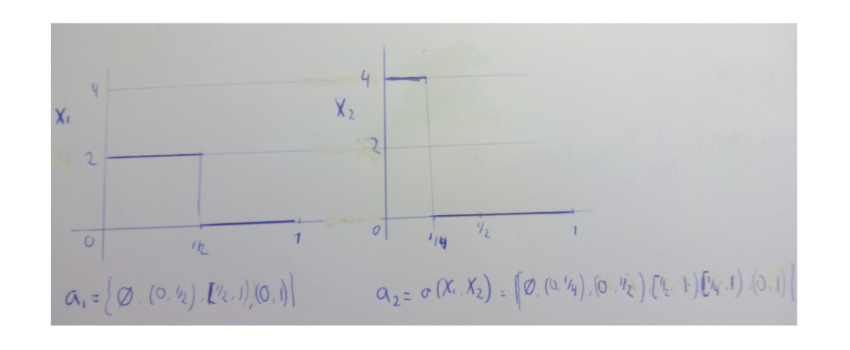
\includegraphics[scale=0.55]{img/grafica1.png}
\end{center}


$$
\mathbb{E}(X_1|\algb{A}_1)(w)
  \left\lbrace
  \begin{array}{l}
     2 \text{ si } w \in (0,\frac{1}{2}) \\
     0 \text{ si } w \in [\frac{1}{2}, 1) \\
  \end{array}
  \right. \text{   }
\mathbb{E}(X_2|\algb{A}_1)(w)
    \left\lbrace
    \begin{array}{l}
       2 \text{ si } w \in (0,\frac{1}{2}) \\
       0 \text{ si } w \in [\frac{1}{2}, 1) \\
    \end{array}
    \right.
$$
$$
\mathbb{E}(X_2|\algb{A}_1)(w) = \mathbb{E}(X_1|\algb{A}_1)(w) = X_1(w) \text{ por ser } X_1 \text{ } \algb{A}_1\text{-medible}
$$

Se cumple que $\algb{A}_n = \sigma(X_1, X_2,...,X_n)$ es una $\salgb$ generada por una partición, de modo que: $\algb{A}_n=\sigma((0,\frac{1}{2}),[\frac{1}{2}, 1),(0,\frac{1}{4}),[\frac{1}{4}, 1), (0,\frac{1}{2^n}),[\frac{1}{2^n}, 1)) = \sigma((0,\frac{1}{2^n}), [\frac{1}{2^n}, \frac{2}{2^n}),...,[\frac{2^n -1}{2^n},1))$

Y se puede aplicar la definición de esperanzas condicionadas a $\salgb$ generadas por particiones:

\[
\mathbb{E}(X_{n+1}|\algb{A}_n)(w)=\sum_{i=1}^{2^n}\left( \frac{1}{P(A_i)}\int X_{n+1}(w)dP(w)\right)\ind_{A_i(w)}
\]

Siendo $A_i$ el intervalo $(\frac{i-1}{2^n}, \frac{i}{2^n})$ y $X_{n+1}$ una variable aleatoria que vale $2^{n+1}$ en el intervalo $(0, \frac{1}{2^{n+1}})$ y 0 en el resto, tenemos que:

$$
\mathbb{E}(X_{n+1}|\algb{A}_n)(w)
  \left\lbrace
  \begin{array}{l}
     \frac{2^{n+1}}{2}=2^n \text{ si } w \in (0,\frac{1}{2^n}) \\
     0 \text{ si } w \in [\frac{1}{2^n}, 1) \\
  \end{array}
  \right. \text{   }
$$

Por tanto nos queda que: $\mathbb{E}(X_{n+1}|\algb{A}_n)=X_n$, y vemos que se cumple la propiedad 3 de las martingalas.

\end{proof}

Sin embargo X no es una martingala en $L^p$ para $p>1$:
\begin{proof}
Hay que ver si $\norm{X}_p = \sup_{n\geq 0}\left(\mathbb{E}(\abs{X_n}^p) \right)^\frac{1}{p} < \infty$. Sin embargo esto no ocurre:

\[
\left(\mathbb{E}(\abs{X_n}^p) \right)^\frac{1}{p} = \left(\int_{0}^{1} 2^{np} \ind_{(0,\frac{1}{2^n})}^p dx\right)^\frac{1}{p} = 2^n \left(\int_{0}^{1} \ind_{(0,\frac{1}{2^n})} dx\right)^\frac{1}{p} =
\]

\[
= 2^n \left( \frac{1}{2^n} \right)^\frac{1}{p} = 2^{n(1-\frac{1}{p})} = 2^{\frac{n}{q}} \stackrel{n \rightarrow \infty}{\rightarrow} \infty
\]

Siendo q el conjugado de p (1/p + 1/q = 1). Y tenemos que $\norm{X}_{\infty} = \infty$.
\end{proof}

\end{example}

Para entender bien la siguiente definición y teorema, se recomiendo ver el ejercicio 4.6:

\begin{defn}[Tiempo de parada]
Sea $\{\algb{A}_n \}_{n \geq 0}$ una filtración. $T: \Omega \rightarrow \mathbb{N}\cup \{\infty \}$ es un tiempo de parada si $\forall n \geq 0, \{w \in \Omega \text{ tal que } T(w)=n\} \in \algb{A}_n$.
\end{defn}

\begin{theorem}[Teorema de parada opcional de Doob]

Sea $X=\{\{X_n\}_{n=1}^{\infty}, \{\algb{A}_n\}_{n=0}^{\infty}\}$ una martingala. Entonces $\mathbb{E}(X_0)=\mathbb{E}(X_t)$ si se cumple cualquiera de las condiciones siguientes:
\begin{enumerate}
\item $\exists M >0$ tal que $T \leq M$. (es decir, la función T tiene máximo)
\item $\forall n \geq 0$ y casi todo $w \in \Omega$, $\abs{X_n(w)} \leq M$ con $M >0$ fijo.
\item $\mathbb{E}(T)<\infty$ y $\exists M > 0$ tal que para casi todo w y todo n $\abs{X_{n+1}(w) - X_n(w)} \leq M$.
\end{enumerate}
\end{theorem}

\begin{theorem}[Teorema de la convergencia de las martingalas de Doob]

Sea $X=\{\{X_n\}_{n=1}^{\infty}, \{\algb{A}_n\}_{n=0}^{\infty}\}$ una martingala en $L^1$. Entonces $X_{\infty}=\lim_{n \rightarrow \infty} X_n$ existe casi seguro. Y además $\mathbb{E}(\abs{X_{\infty}})<\infty$, luego $P(\abs{X_{\infty}}=\infty)=0$.

\obs  esto no implica que $X_n$ converja a $X_{\infty}$ en $L^1$.

\end{theorem}


\begin{proof}
No lo vamos a demostrar bien, solo algún comentario. Sabiendo que $X_{\infty}=\lim_{n \rightarrow \infty} X_n$ existe, entonces por Fatou:
\[
\mathbb{E}(\abs{X_{\infty}}) = \mathbb{E}(\abs{\lim_{n \rightarrow \infty} X_n}) \leq \mathbb{E}(\lim_{n \rightarrow \infty} \abs{X_n}) =
\]

\[
= \mathbb{E}(\liminf_{n \rightarrow \infty} \abs{X_n}) \leq \liminf_{n \rightarrow \infty} \mathbb{E}(\abs{X_n}) \leq \sup_n \mathbb{E}(\abs{X_n}) <\infty
\]

Ya que $X \in L^1$

\end{proof}

Ahora vamos a ver el contraejemplo para la observación:
\begin{proof}
Sea X la martingala que hemos visto anteriormente, con $X_n=  2^n \ind_{(0, \frac{1}{2^n})}$, hemos visto que X pertenece a $L^1$. Y tenemos que $\lim_{n \rightarrow \infty} X_n = X_{\infty} = 0$.

Breve nota de por qué ese es el límite: estamos calculando el límite puntual de las funciones $X_n$ y esta claro que si elijo un $\epsilon >0$, para todo x voy a encontrar un $N_{\epsilon x}$ tal que para todo $m \geq N_{\epsilon x}$, se cumple que $X_m(w)$ es 0. Por ejemplo para $x=\frac{1}{4}$, a partir de $X_2$, ya todas las funciones $X_{n>2}$ son 0, es decir $\lim_{n \rightarrow \infty} X(\frac{1}{4})=0$. Por tanto hay convergencia puntual, pero en este caso no la hay uniforme, ya que no para todo $\epsilon$, $X_n(w)<\epsilon$ para todos los w (siempre va a haber un intervalo pequeño en el origen que va a valer bastante, por ejemplo $X_n$ va a valer $2^n$ en el intervalo $(0, \frac{1}{2^n})$.

Ahora vamos a ver que  $X_n \stackrel{L^1}{\nrightarrow} X_{\infty}$ ya que se tiene que cumplir que $\int_{\Omega} \abs{X_n - X_{\infty}} \rightarrow 0$, y sin embargo:
\[
\lim_{n \rightarrow \infty} \int_{\Omega} \abs{X_n - X_{\infty}} = \lim_{n \rightarrow \infty} \int_{\Omega} \abs{X_n - 0} = \lim_{n \rightarrow \infty} \mathbb{E}(\abs{X_n}) = \lim_{n \rightarrow \infty} 1 = 1
\]

Vemos que no podemos aplicar el TCM ni TCD y escribir: $\lim_{n \rightarrow \infty} \mathbb{E}(\abs{X_n}) =  \mathbb{E}(\abs{\lim_{n \rightarrow \infty} X_n}) = 0$, ya que $X_n$ no es una sucesión creciente ni existe una $g \in L^1$ tal que $\abs{X_n} \leq g$, y por tanto no cumple las condiciones de ninguno de los teoremas.

\end{proof}

\begin{theorem}[Teorema de la convergencia de las martingalas de Doob en $L^p$ para p>1]

Sea $X=\{\{X_n\}_{n=1}^{\infty}, \{\algb{A}_n\}_{n=0}^{\infty}\}$ una martingala en $L^p$ con p>1. Entonces:
\begin{itemize}
\item $X_{\infty}=\lim_{n \rightarrow \infty} X_n$ existe casi seguro.
\item $X_n \stackrel{L^p}{\rightarrow} X_{\infty}$.

\item $X_{\infty}$ es $\algb{A}$-medible y $X_n=\mathbb{E}(X_{\infty}|\algb{A}_n)$
\end{itemize}
\obs Si $Y \in L^p$ con $1 \leq p \leq \infty$, entonces: $X_n= \mathbb{E}(Y|\algb{A}_n)$ define una martingala. Lo cual es obvio ya que si $Y \in L^p$, la esperanza, que no es mas que una contracción de Y, también pertenecerá a $L^p$. Y podemos aplicar la definición vista anteriormente (martingala en $L^p$).

\end{theorem}

\begin{theorem}
Sea X una martingala en $L^1$, si $X_n \rightarrow X_{\infty}$ en $L^1$, entonces $\mathbb{E}(X_{\infty}|\algb{A}_n)=X_n$.
\end{theorem}
\begin{proof}
Tenemos dos funciones $\algb{A}_n$-medibles, basta probar que $\forall B \in \algb{A}_n$, se cumple que $\int_B X_n = \int_B \mathbb{E}(X_{\infty}|\algb{A}_n) = \int_B X_{\infty}$.

\[
X_n \stackrel{L^1}{\rightarrow} X_{\infty} \Leftrightarrow \lim_{n \rightarrow \infty} \norm{X_{\infty}-X_n}_1=0 \Leftrightarrow 0= \lim_{n \rightarrow \infty} \int_{\Omega}\abs{X_{\infty}-X_n}dP \geq \lim_{n \rightarrow \infty} \int_B \abs{X_{\infty}-X_n}dP\geq
\]

\[
\geq \lim_{n \rightarrow \infty} \abs{\int_B X_{\infty}dP- \int_B X_n dP} \geq 0
\]


Por tanto nos queda que:
\[
\lim_{n \rightarrow \infty} \int_B X_n = \int_B X_{\infty}
\]

Que es lo mismo que decir que:
\[
\lim_{n \rightarrow \infty} \int_B X_n = \lim_{m \rightarrow \infty} \int_B X_{n+m} = \int_B X_{\infty}
\]

Por otro lado hemos visto que: $\mathbb{E}(X_{n+m}|\algb{B}) = X_n$ (ver ejercicio 6 de la hoja 4). Y esto implica (por definición de esperanza condicionada) que $\forall B \in \algb{B}$:
\[
\int_B \mathbb{E}(X_{n+m}|\algb{A}_n)=\int_B X_{n+m} = \int_B X_n
\]

Aplicamos límites y  lo anterior tenemos lo que buscábamos:
\[
\lim_{m \rightarrow \infty}\int_B X_{n+m} = \lim_{m \rightarrow \infty}\int_B X_{n} \Leftrightarrow \int_B X_{\infty} = \int_B X_n
\]

\end{proof}

\chapter{Independencia (Tema 2)}

\textcolor{red}{Apuntes sin completar, faltan 4 clases, se completarán espero antes del 2 de Mayo}

A partir de una sucesión infinita, hay independencia si la hay para todas sus subsucesiones finitas, basta por tanto dar la definición para sucesiones finitas.

\begin{defn}[Independencia de conjuntos]
Los conjuntos $A_1,...,A_n$ son independientes si $\forall$ subsucesión de $\{1,...,n\}$, con $i_1 < i_2 < ... < i_n$, se tiene que:
\[
P(\cap_{j=1}^k A_{ij}) = \prod_{j=1}^{k}P(A_{ij})
\]
\end{defn}

\begin{defn}[Independencia de variables aleatorias]
Las variables aleatorias $X_1, X_2,...,X_n$ son independientes si para toda colección $B_1,...,B_n$ de conjuntos de Borel en $\mathbb{R}$ se tiene que:
\[
P(\cap_{i=1}^n \{X_i \in B_i\})= \prod_{i=1}^{n} P(\{X_i \in B_i\})
\]
\end{defn}

\begin{defn}[Independencia para $\salgb$]
Las $\salgb$ $\algb{A}_1,...,\algb{A}_n$ son independientes si $\forall B_i \in \algb{A}_i$ se tiene que:
\[
P(\cap_{i=1}^n B_i) = \prod_{i=1}^{n} P(B_i)
\]
\end{defn}

\begin{defn}[Independencia para colecciones de conjuntos]
Las colecciones de conjuntos $C_1,...,C_n$ son independientes si para toda subsucesión $C_{i1},...,C_{ik}$ y $B_{i1} \in C_{i1},..., B_{ik} \in C_{ik}$, se cumple que:
\[
P(\cap_{j=1}^n B_{ij})=\prod_{j=1}^{n}P(B_{ij})
\]
\end{defn}

\obs $X_1,...,X_n$ son independientes $\Leftrightarrow$ $\sigma(X_1),...,\sigma(X_n)$ son independientes.

\begin{theorem}
Son equivalentes:
\begin{enumerate}
\item X e Y son independientes.
\item $\forall f,g: \mathbb{R} \rightarrow \mathbb{R}$ funciones de Borel acotadas (integrales bien definidas), entonces:
\[
\mathbb{E}(f(X)g(Y))=\mathbb{E}(f(X))\mathbb{E}(g(Y))
\]
\item $\forall f,g: \mathbb{R} \rightarrow [0, \infty)$ funciones de Borel, entonces:
\[
\mathbb{E}(f(X)g(Y))=\mathbb{E}(f(X))\mathbb{E}(g(Y))
\]
\item  $\forall f,g: \mathbb{R} \rightarrow \mathbb{R}$ funciones de Borel tal que $\mathbb{E}(|f(X)|)<\infty$ y $\mathbb{E}(|g(Y)|)<\infty$, entonces:
\[
\mathbb{E}(f(X)g(Y))=\mathbb{E}(f(X))\mathbb{E}(g(Y))
\]
\end{enumerate}
\end{theorem}

\textbf{Corolario}: Si $X,Y \in L^1$ y son independientes, entonces: $\mathbb{E}(XY)=\mathbb{E}(X)\mathbb{E}(Y)$ (f=g=id)

\textbf{Comentario}: El resultado análogo para funciones de variables variables y variables aleatorias independientes también es cierto. Por ejemplo, si $X_1,...,X_5$ son independientes y $f:\mathbb{R}^2 \rightarrow \mathbb{R}$ y $g:\mathbb{R}^3 \rightarrow \mathbb{R}$ son funciones de Borel acotadas, entonces:
\[
\mathbb{E}(f(X_1,X_2),g(X_3,X_4,X_5))= \mathbb{E}(f(X_1,X_2)) \mathbb{E}(g(X_3,X_4,X_5))
\]

\begin{defn}[covarianza e incorrelación]
\begin{itemize}

\item cov(X,Y)=$\mathbb{E}((X-\mathbb{E}(X))(Y-\mathbb{E}(Y)))=\mathbb{E}(XY)-\mathbb{E}(X)\mathbb{E}(Y)$.

\item$X,Y$ son incorrelacionadas si cov(X,Y)=0 $\Leftrightarrow \mathbb{E}(XY)=\mathbb{E}(X)\mathbb{E}(Y) $

\item$X,Y$ independientes $\Rightarrow X,Y$ incorrelacionadas. Implicación contrario no siempre cierta.
\end{itemize}
\end{defn}

\obs Si X e Y están en $L^2$ (Aplicación de Pitágoras), entonces:
\[
cov(X,Y)=0 \Leftrightarrow X-\mathbb{E}(X) \perp Y - \mathbb{E}(Y)
\]

\obs SI $X_1,...,X_n$ son incorrelacionadas entonces:
\[
var(\sum_{i=1}^{n} X_i) = \sum_{i=1}^{n}var(X_i)
\]
\begin{proof}
Por definición $var(X)=\mathbb{E}((X-\mathbb{E}(X))^2)$

\[
var(\sum_{i=1}^{n} X_i) = \mathbb{E}\left((\sum_{i=1}^{n} X_i  -\mathbb{E}(\sum_{i=1}^{n}X_i))^2\right) = \mathbb{E}\left((\sum_{i=1}^{n} (X_i  -\mathbb{E}(X_i)))^2\right) =
\]
\[
= \sum_{i=1}^{n}( \mathbb{E}(X_i  -\mathbb{E}(X_i)))^2= \sum_{i=1}^{n} Var(X_i)
\]

El primer y segundo paso es por definición de varianza y el penúltimo paso se debe a Pitágoras. Ver ejercicio 3 de la hoja 6.
\end{proof}

\begin{theorem}
Sean $C=C_1,...,C_n$ colecciones de conjuntos, cada una de ellas cerradas por intersecciones finitas, es decir, si $A,B \in C_i$, entones $A \cap B \in C_i$ para cualquier $i\geq1 , i \leq n$. Si $C_1,...,C_n$ son independientes, entonces $\sigma(C_1),...,\sigma(C_n)$ son independientes. La implicación contraria es obviamente cierta.
\end{theorem}

Notación: $\sigma(X_1,X_2)=\sigma(\sigma(X_1),\sigma(X_2))$  es la $\salgb$ más pequeña que hace que tanto $X_1$ como $X_2$ sean medibles. Que no es lo mismo que $\sigma(X_1\cdot X_2)$ lo cual se refiere a la $\salgb$ que hace que $X_1\cdot X_2$ sea medible.

\begin{example}
Sean $X_1, X_2, X_3, X_4$, variables aleatorias independientes..Entonces $\sigma(X_2 \cdot X_3 \cdot X_4) \subset \sigma(\sigma(X_2),\sigma(X_3),\sigma(X_4))$. Luego por el teorema anterior:

$\sigma(X_1)$ y $\sigma(X_2 \cdot X_3 \cdot X_4)$ son independientes $\Leftrightarrow X_1 \text{ y } X_2X_3X_4$ son independientes. Y esto implicaría que $\mathbb{E}(X_1X_2X_3X_4)=\mathbb{E}(X_1)\mathbb{E}(X_2X_3X_4)$. \textcolor{red}{¿Donde usamos el teorema?}
\end{example}

\begin{defn}
Dado el vector aleatorio $(X_1,...,X_n)$, su función de distribución es $F_{X_1,...,X_n}(t_1,...,t_n)=P(X_1 \leq t_1, X_2 \leq t_2,...,X_n \leq t_n)$
\end{defn}

\textbf{Corolario}: son equivalentes:
\begin{enumerate}
\item $X_1,...,X_n$ son independientes..
\item $\forall(t_1,...,t_n) \in \mathbb{R}^n, P(\cap_{i=1}^n \{X_i \leq t_i\})=\prod_{i=1}^{n}P(X_i \leq t_i)$
\item $\forall(t_1,...,t_n) \in \mathbb{R}^n, F_{X_1,...,X_n}(t_1,...,t_n)=\prod_{i=1}^{n}F_{X_i}(t_i)$
\end{enumerate}

\begin{proof}
\begin{itemize}
\item $2 \Leftrightarrow 3$ es notación.
\item $1 \Leftrightarrow 2$ es trivial.
\item $2 \Leftrightarrow 1$ Las clases $C_i=\{\{X_i \leq t\}:t \in \mathbb{R}\}$ están cerradas por intersecciones finitas y son independientes $\Leftrightarrow$ 
\end{itemize}
\end{proof}

\textbf{Corolario:} Si $X_1,...,X_n$ son independientes y $f:\mathbb{R}^k \rightarrow \mathbb{R}$ y $g:\mathbb{R}^{n-k}\rightarrow \mathbb{R}$ son funciones de Borel, entonces $f(X_1,...,X_k)$ y $g(X_{k+1},...,X_n)$ son independientes.

\begin{proof}
Veamos que $\sigma(f(X_1,...,X_k))$ y $\sigma(g(X_{k+1},...,X_n))$ son independientes, entonces:
\begin{itemize}
\item $\sigma(f(X_1,...,X_k)) \subset \sigma(\sigma(X_1),...,\sigma(X_k))$
\item $\sigma(g(X_{k+1},...,X_n)) \subset \sigma(\sigma(X_{k+1}),...,\sigma(X_n))$
\end{itemize}

Cerramos $\sigma(X_1),...,\sigma(X_k)$ por intersecciones finitas, hacemos lo mismo con $\sigma(X_{k+1},...,\sigma(X_n))$ y aplicamos el teorema 
\end{proof}

\begin{example}
$f(x)=x$ y $g(x,y,z)=xyz$, son funciones de Borel porque son continuas. Si $X_1, X_2, X_3, X_4$ son independientes entonces $X_1$ y $X_2X_3X_4$ también lo son po el corolario anterior. 
\end{example}

\begin{theorem}
Sea $\algb{A}$ un álgebra de conjuntos. Entonces todo conjunto de $\sigma(\algb{A})$ es aproximable.
\end{theorem}

\begin{defn}
Un conjunto B es aproximable si $\forall \epsilon >0$, $\exists A=A(\epsilon) \in \algb{A}$ tal que $P(A \bigtriangleup B) < \epsilon$ o equivalentemente, $\exists \{A_n\}_{n\geq 1}$ de conjuntos en $\algb{A}$ tal que $\lim_{n \rightarrow \infty}P(A_n \bigtriangleup B)=0$.

Notación: $A \bigtriangleup B$ indica la diferencia simétrica de A con B.
\end{defn}

\begin{proof}
Es fácil ver que si $B \subset \Omega$ es aproximable, entonces $B^c$ es aproximable y que si $B_1,B_2,...$ son aproximables entonces $\cup_{n\geq1} B_n$ es aproximable. En este caso se observa que dado $\epsilon >0$, $\exists n$ tal que $P(\cup_{n\geq1}B_n)-P(\cup_{n=1}^NB_n)<\frac{\epsilon}{2}$.

Como la clase de conjuntos aproximables contiene a $\algb{A}$, está cerrada por complementación y por uniones numerables, entonces contiene a $\sigma(\algb{A})$. 
\end{proof}

\begin{defn}[[$\sigma$-álgebra asintótica]
Sea $C_1, C_2, C_3,...$ una sucesión de colecciones de conjuntos y sea $B_n=\sigma(\cup_{k\geq n}C_k)$, se observa que $B_n$ es decreciente porque cada vez esta generada por menos conjuntos. De modo que la $\salgb$  $\cap_{n\geq 1}B_n=B_{\infty}$ se denomina $\salgb$ asintótica o terminal relativa a $C_1, C_2,...$
\end{defn}

\begin{example}
Sea $\{X_n\}_{n=1}^{\infty}$ una sucesión de variables aleatorias y sea $C_i=\sigma(X_i)$. Consideramos $A= \{w \in \Omega:\lim_{n \rightarrow \infty} \frac{1}{n}\sum_{i=1}^{n} X_i(w)$ existe$\}$. Entonces, ese conjunto A, pertenece a $B_{\infty}$.
\end{example}

\begin{defn}[límite superior e inferior]
\begin{itemize}
\item $\limsup_{n \rightarrow \infty}A_n= \{w \in \Omega: w \in A_n$ para infinitos $n \in \mathbb{N} \}$=$\cap_{k \geq 1}\cup_{n\geq k} A_n$.

\obs $\limsup_{n \rightarrow \infty} \ind_{A_n}=\ind_{\limsup_{n \rightarrow \infty} A_n}$

\item $\liminf_{n \rightarrow \infty}A_n= \{w \in \Omega: w \in A_n \forall n$ salvo quizás un conjunto finito de ellos $n \in \mathbb{N} \}$=$\cup_{k \geq 1}\cap_{n\geq k} A_n$.
\end{itemize}
\end{defn}

\begin{example}
Si $A_n \in C_n$, entonces $A_n \in B_m \forall n\geq m$ y $\limsup_n A_n$ y $\liminf_n A_n$ pertenecen a $B_{\infty}$ 
\end{example}

\textbf{Ley 0-1 de Kolgomorov}: Sea $C_1, C_2,...$ sucesión de colecciones independientes de conjuntos en $\Omega$, cada una de ellas cerradas por intersecciones finitas.

Sea:
\begin{itemize}
\item $\algb{A}_n=\sigma(\sigma(C_1),...,\sigma(C_{n-1})$ con $n\geq 2$
\item $\algb{B}_n=\sigma(\cup_{k\geq n} \sigma(C_k))$ con $n\geq 2$
\end{itemize} 

Sabemos que $\algb{A}_n$ y $\algb{B}_n$ son $\salgb$s independientes, de modo que si $A \in B_{\infty}$ entonces $P(A)=0$ ó 1
\begin{proof}
Supongamos que $\exists n$ tal que $\forall A \in \algb{A}_n$.  Como $A \in \algb{B}_n$, A es independiente de sí mismo. Por tanto:
\[
P(A)=P(A\cap A)=P(A)\cdot P(A) \Rightarrow P(A)-P(A)\cdot P(A)=0 \Rightarrow
\]
\[
\Rightarrow P(A)\cdot(1-P(A))=0 \Rightarrow P(A)=0 \text{ ó } 1
\]

También sabemos que si $A \in B_{\infty}$, entonces $A \in B_2 = \sigma(\cup_{k\geq 2}\sigma(C_k))$.

Sea $\algb{A}$ el álgebra generada por $\cup_{k\geq 2}(\sigma(C_k))$ puede demostrarse que todo conjunto en $\algb{A}$ es aproximable por conjuntos en $\cup_{i\geq 2} \sigma(C_i)$. Dado A puede aproximarse, por el teorema, de modo que, $\exists A_{nj} \in \algb{A}$ tal que $\lim_j P(A_{nj}\bigtriangleup A)=0$.

De manera que $A_{nj}$ se aproxima a A cuando la j tiende a infinito. Además $A_{nj}\in \algb{A}_{nj}$ que es independiente de $A \in \algb{B}_{nj}$, y por esto, tenemos que:
\[
\lim_{j \rightarrow \infty}P(A_{nj})\cdot P(A)=P(A)^2= \lim_{j \rightarrow \infty}P(A_{nj} \cap A)=P(A)
\]

\textcolor{red}{Preguntar por esta demostración a Munarriz con los apuntes de elena delante, y por los ejemplos de debajo}
\end{proof}

\begin{example}
Sea $A_n$ una sucesión de eventos o sucesos independientes, tenemos que:
\[
P(\limsup_{n \rightarrow \infty}A_n) = 0 \text{ ó } 1
\]
\end{example}

\begin{theorem}[Teorema de Borel-Cantelli]
Hay dos enunciados:
\begin{enumerate}
\item \textbf{Teorema de Borel-Cantelli I} (No requiere independencia): Sea $\{A_n\}_{n=0}^{\infty}$ una sucesión de conjuntos tal que $\sum_{n=1}^{\infty}P(A_n)< \infty$, entonces $P(\limsup_{n \rightarrow \infty}A_n)=0$.

\item \textbf{Teorema de Borel-Cantelli II} (Sí requiere independencia): Sea $\{A_n\}_{n=0}^{\infty}$ una sucesión de conjuntos independientes tal que $\sum_{n=1}^{\infty}P(A_n)= \infty$, entonces $P(\limsup_{n \rightarrow \infty}A_n)=1$.
\end{enumerate}
\end{theorem}
\begin{proof}
Consultar el apartado de teoremas para el examen para ver la demostración.
\end{proof}

\section{Funciones de distribución: $F_X(t)=P(X\leq t)=P_X((-\infty,t])$}
Hay 3 tipos puros:

\begin{enumerate}
\item Distribuciones discretas: X tiene distribución discreta si $\exists$ un conjunto numerable $D\subset \mathbb{R}$ tal que $P_X(D)=1$

Algunas distribuciones discretas son Bernouilli, Binomial, Poisson...


\begin{example}
Un ejemplo sencillo es el siguiente: En el espacio de probabilidad $([0,1], Borel, \lambda)$, defino $X_n:[0,1]\rightarrow[0,1]$, con $X_n(w)=1/n$.

\begin{center}
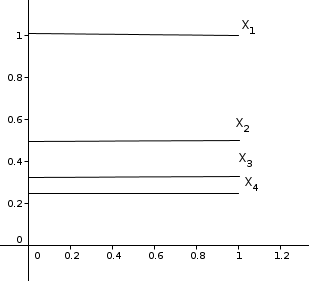
\includegraphics[scale=0.4]{img/g1.png}
\end{center}

Se trata de una variable aleatoria que es constante para todo w. Es obvio que $X_n \rightarrow 0$ en todos los sentidos posibles.

Esta claro que converge uniformemente, y por tanto lo hace en $L^p$ y en todo punto. Por ello también converge en probabilidad, y por converger en probabilidad también converge en distribución.

Además, la función de probabilidad $P_{X_n}=\delta_{\frac{1}{n}}$ (delta de Dirac) pues la probabilidad de un evento w tal que $X_n(w)>\frac{1}{n}$ o $X_n(w)<\frac{1}{n}$ es 0, y P(w) tal que $X_n(w)=\frac{1}{n}$ es 1.

La función de distribución quedaría de la siguiente manera.

$$
F_{X_n}(t) =
  \left\lbrace
  \begin{array}{l}
     1 \text{ si } t \geq \frac{1}{n}\\
     0 \text{ si } t < 1 \\
  \end{array}
  \right.
$$

Mostramos $F_{X_1}$ y $F_{X_2}$:

\begin{center}
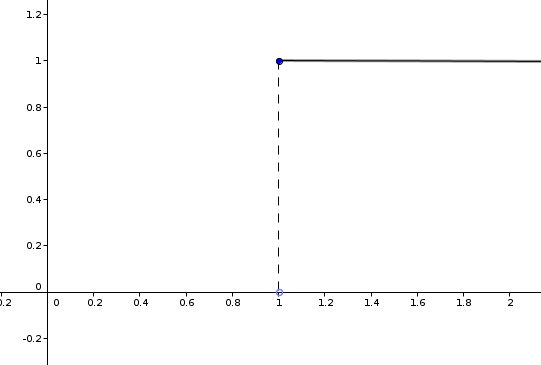
\includegraphics[scale=0.4]{img/g2.png}
\end{center}

\begin{center}
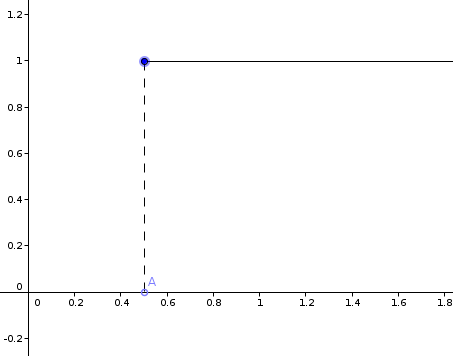
\includegraphics[scale=0.4]{img/g3.png}
\end{center}

Y definimos $F_0$ de la siguiente manera:

\begin{center}
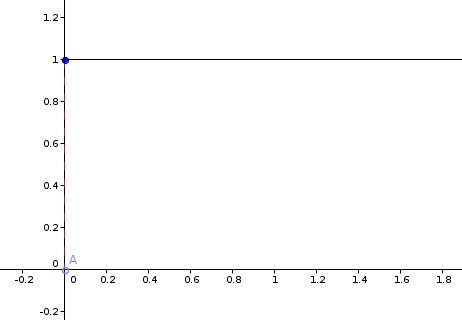
\includegraphics[scale=0.4]{img/g4.png}
\end{center}

Y vemos que:

\[
\lim_{n \rightarrow \infty} F_{X_n}(0)=0<1=F_0(0)
\]

\[
\lim_{n \rightarrow \infty} F_{X_n}(t)=F_0(t) \text{ para t $\neq 0$}
\]

Por tanto, $X_n \stackrel{D}{\rightarrow} 0$ en distribución también. (Recordar la definición de convergencia en distribución vista en el primer tema de "nociones básicas").

\end{example}

\item Distribuciones continuas, $F_X$ es absolutamente continua, es decir, el TFC (Teorema Fundamental del Cálculo) es válido para $F_X$ si dado $a<b$: $F_X(b)-F_X(a)=\int_{a}^{b} F_X'(t) dt$. Entonces $f_X(t)=F_X'(t)$ existe en casi todo punto (Siendo $f_X$ la función de densidad de X). 

También se puede escribir $P<<\lambda$, que quiere decir (como vimos en el tema 1) que si $\lambda(A)=0 \Rightarrow P(A)=0$.

Algunos ejemplos son la distribución uniforme o la normal.

\obs Por definición de independencia y utilizando el TFC y Fubini en el último paso, tenemos que:
\[
X \text{ e } Y \text{ son independientes } \Leftrightarrow F_{(X,Y)}(a,b)=F_X(a)\cdot F_Y(b) \Leftrightarrow f_{(X,Y)}(a,b)=f_X(a)\cdot f_Y(b)
\]

\item $F_X$ es continua singular. $F_X$ es continua y $F'_X=0$ en casi todo puno con  respecto a la medida de Lebesgue $\lambda$. Y ocurre que $\int_{a}^{b} F_X'(t) dt = 0$ (a diferencia que en las distribuciones continuas, que era F(a)-F(b)). En términos de $P_X$ quiere decir que existe un conjunto tal que su probabilidad es 1 y su medida de lebesgue es 0: $\exists A \subset \mathbb{R}$ tal que $P_X(A)=1$ y $\lambda(A)=0$.

\begin{example} 
El ejemplo más típico es la función de Cantor, que tiene medida Lebesgue 0 pero no de probabilidad. Recordar que una función de Cantor es aquella en la que tenemos el intervalo $[0,1]$ y quitamos el tercio central. Después de los dos intervalos que nos quedan, quitamos el central, y así sucesivamente. Al final, la medida de Lebesgue del conjunto será 0, pero la función de probabilidad la puedes definir como quieras. \textcolor{red}{Preguntar un poco por esto a munarriz}
\end{example}
\end{enumerate}

Con esta información, podemos enunciar el siguiente teorema:
\begin{theorem}
Toda función de distribución $F_X$ es combinación convexa de una función de distribución discreta, otra absolutamente continua y una tercera continua y singular, es decir, $\exists a,b,c \geq 0$ con $a+b+c=1$, tal que:
\[
F_X=aF^{discreta}+bF^{\text{absolutamente continua}}+cF^{\text{continua singular}}
\]
\end{theorem}

\textbf{Configuraciones triangulares de v.a.:}
De forma general se define una  configuración triangular de la siguiente manera:
\\
$X_{1,1},...,X_{1,m(1)}$\\
$X_{2,1}, X_{2,2},...,X_{2,m(2)}$\\
$X_{3,1}, X_{3,2}, X_{3,3},...,X_{3,m(3)}$\\
.\\
$X_{n,1}, X_{n,2},...,X_{n,n},...,X_{n,m(n)}$

Con 'm(x)' estrictamente creciente. \textcolor{red}{Y que?}

\begin{example}
Sea $Y\sim Poisson(\lambda) \Rightarrow \mathbb{E}(Y)=\lambda=Var(Y)$. Es útil para aproximar $S_n \sim B(n,p)$.

Tenemos que $\mathbb{E}(S_n)=np$ y $Var(S_n)=np-np^2$ pues sabemos que $X_i \sim Ber(p)$ con $Var(X_i)=p-p^2$.

Para que la Poisson sea una buena aproximación de la $Binomial(n,p)$ tendremos que escoger: $\lambda=np$ y como queremos que $np=Var(Y)\approx Var(S_n)=np-np^2 \Rightarrow np^2\approx0$.

Mediante el siguiente teorema generalizamos la aproximación de $S_n \sim B(n,p)$ por $Y\sim Poisson(np)$.
\end{example}

\begin{theorem}[Ley de números pequeños]
Para $n=1,2,3,...$ sea $\{X_{n,1},X_{n,2},...,X_{n,n}\}$ una sucesión finita de pruebas de Bernoulli independientes con $P(X_{n,m}=1)=P_{n,m}$. Si se cumplen las siguientes condiciones:
\begin{enumerate}
\item $\lambda=\lim_{n \rightarrow \infty} \sum_{m=1}^{n}P_{n,m}$ existe y satisface $0<\lambda<\infty$.
\item $\lim_{n \rightarrow \infty} \max\{P_{n,1},...,P_{n,m}\}=0$
\end{enumerate}
Entonces: 
\[
\sum_{m=1}^{n}X_{n,m} \stackrel{D}{\rightarrow} Y \text{ cuando $n \rightarrow \infty$}
\]
\end{theorem}

\section{Distribución normal multivariante}
\text{Notación:}
\begin{itemize}
\item $X=(X_1,...,X_n)$ un vector aleatorio con $\mu=(\mu_1,\mu_2,...,\mu_n)$ donde $\mu_i=\mathbb{E}(X_i)$
\item Matriz de covarianzas: $\wedge=[Cov(X_i,X_j)]_{1\leq i, j\leq n}$
\end{itemize}

\textbf{Recordatorio:} 
\begin{itemize}
\item con n=1: $$X\sim N(\mu, \sigma) \Leftrightarrow f_X(x)=\frac{1}{\sigma \sqrt{2\pi}}e^{-\frac{(x-\mu)^2}{2\sigma^2}}$$
\item con n>1, $X=(X_1,...,X_n)$ y tenemos que: $$X\sim N(\mu, \wedge) \Leftrightarrow f_X(x)=\frac{1}{\sqrt{det\wedge}(2\pi)^{n/2}}e^{-\frac{1}{2}[x-\mu]^T \wedge{-1}[x-\mu]}$$
\item $A^{nxn}$ es semidefinida positiva si $\forall x \in \mathbb{R}^n$ se cumple que $x^TAx \geq 0$.
\end{itemize}

\obs $Cov(X,Y)=Cov(Y,X)$ ya que $\mathbb{E}(XY)-\mathbb{E}(X)\mathbb{E}(Y)=\mathbb{E}(YX)-\mathbb{E}(Y)\mathbb{E}(X)$. Y entonces $\wedge$ es una matriz simétrica y semidefinida positiva: $c\geq0 \Leftrightarrow \forall x \in \mathbb{R}cx^2\geq0$

\begin{theorem}
Sea $X \sim$ Normal multivariante, con $X=(X_1,...,X_n)$. Las variables $X_1,...,X_n$ tienen distribución normal (en dimensión 1). Además son incorrelacionadas $\Leftrightarrow $ son independientes.
\end{theorem}
\begin{proof}
\begin{itemize}
\item $\Leftarrow)$ obvio
\item $\Rightarrow)$ Usaremos que $\wedge$ es diagonal (pues son incorrelacionadas: $Cov(X_i,,X_j)=0 si i\neq j$. $\wedge{-1}$ también es diagonal (con las entradas inversas). Entonces:
\[
e^{f_1(X_1)+f_s(X_2)+...+f_n(X_n)}=\prod_{i=1}^{n}e^{f_i(X_i)}
\]

Por lo que:
\[
f_X(X)=f_{X_1}(X_1)...f_{X_n}(X_n)
\]
\end{itemize}
\end{proof}




\chapter{Momentos y desigualdades (Tema 3)}
Desigualdades de Hölder, Minkowsky y Jensen ya vistas (ver hoja de ejercicios número 3). Pero las recordamos igualmente:
\begin{itemize}
\item Desigualdad de Hölder (ver ejercicio 3.3): (Para p y q conjugados) si $f\in L^p$ y $g\in L^q$, entonces $fg\in L^1$, y $\|fg\|_1 \le \|f\|_p\|g\|_q$.
\item Desigualdad de Minkowsky (ver ejercicio 3.5) Para $1<p<\infty$ se cumple:
 $\|f + g\|_p \le \|f\|_p + \|g\|_p$.
\item Desigualdad de Jensen:
\begin{itemize}
\item $X: \Omega \rightarrow I$ (intervalo) una variable aleatoria en $L^1(\Omega, \algb{M},P)$.
\item $\phi: I \rightarrow \mathbb{R}$ convexa, tal que $\phi(X) \in L^1(\Omega,\algb{M},P)$.
\begin{enumerate}
\item $\phi(\mathbb{E}(X)) \leq \mathbb{E}(\phi(X))$
\item $\phi(\mathbb{E}(X|\algb{B})) \leq \mathbb{E}(\phi(X)|\algb{B})$

\end{enumerate}


\end{itemize}
\item Para $1<r$:
$$\left(\int \abs{f}\right)^r \leq\int \left( \abs{f} \right)^r$$

Esto se tiene por jensen y también por definición de varianza:
\[
Var(X)=\mathbb{E}[(X-\mathbb{E}(X))^2] = \mathbb{E}(X^2) - \mathbb{E}(X)^2 \geq 0
\]
\end{itemize}


\begin{defn}[Momento n-ésimo de X]
El momento n-ésimo de X es $\mathbb{E}(X^n)$ para $n=0,1,2,...$.  Para $\alpha \in \mathbb{R}$ el momento absoluto de orden $\alpha$ es $\mathbb{E}(\abs{X}^{\alpha})$.

Vimos que si $0 < r < s \leq \infty$, entonces:
\[
(\mathbb{E}(\abs{X}^r))^{\frac{1}{r}} \leq (\mathbb{E}(\abs{X}^s))^{\frac{1}{s}} \Rightarrow \text{ si } \mathbb{E}(\abs{X}^s) < \infty \Rightarrow \mathbb{E}(\abs{X}^r) < \infty
\]

\begin{expla}
Para ver la desigualdad anterior repasar normas y darse cuenta de que:
\[
\norm{X}_r = (\int \abs{X}^r)^{\frac{1}{r}} = (\mathbb{E}(\abs{X}^r))^{\frac{1}{r}}
\]

Y de que para $0 < r < s \leq \infty$ se cumple que:
\[
\norm{X}_r < \norm{X}_s
\]
\end{expla}
\end{defn}

\begin{defn}[Desigualdad de Markov]
Válida para cualquier medida $\mu$. si $f \geq 0$, entonces $\forall t > 0$ se cumple que $\mu\{f \geq t\} \leq \frac{1}{t}\int f d\mu$

\begin{proof}
\[
\mu\{f \geq t\} = \int \ind_{\{f \geq t\}} d\mu \leq \int_{\{f \geq t\}} \frac{f}{t} d\mu \leq \frac{1}{t}\int_{\Omega}f d\mu
\]
\end{proof}

Si escogemos $\mu=P$, y $f=\abs{X}$, por Markov tendríamos que: $P(\abs{X}\geq t) \leq \frac{1}{t} \mathbb{E}(\abs{X})$
\end{defn}

\obs $P(\abs{X}\geq t) = P(\abs{X}^{\alpha}\geq t^{\alpha}) \leq \frac{1}{t^{\alpha}} \mathbb{E}(\abs{X}^{\alpha}) \text{ } \forall \alpha \in \mathbb{R}$

\obs Para $t>0$, tenemos un caso especial de la desigualdad anterior usando $\alpha=2$ y $X=Y-\mathbb{E}(Y)$. Se denomina desigualdad de Chebishev, es decir:
\[
P(\abs{Y-\mathbb{E}(Y)}\geq t) \leq \frac{Var(Y)}{t^2}
\]
\begin{proof}
\[
P(\abs{Y-\mathbb{E}(Y)}\geq t) = P(\abs{Y-\mathbb{E}(Y)}^2\geq t^2) \leq \frac{1}{t^2}\mathbb{E}(\abs{Y-\mathbb{E}(X)}^2) = \frac{Var(Y)}{t^2}
\]
\end{proof}


\chapter{Modos de convergencia y leyes de los grandes números (Tema 4)}
Las leyes fuertes implican convergencia casi seguro, mientras que las leyes débiles implican convergencia en probabilidad.

Dada una sucesión de variables aleatorias $X_n$ que convergen a X, tenemos las siguientes relaciones de convergencia cuando la n tiende a infinito:

$X_n$ converge a X uniformemente  $\Rightarrow$ $X_n$ converge a X en $L^{\infty}$  $\Rightarrow$ $X_n$ converge a X en $L_p$ para $0<p<\infty$  $\Rightarrow$ $X_n$ converge a X para $0<r<p$  $\Rightarrow$ $X_n$ converge a X en probabilidad  $\Rightarrow$ $X_n$ converge a X en distribución:

\[
X_n \stackrel{uniforme}{\rightarrow} X \Rightarrow X_n \stackrel{L^{\infty}=\norm{.}_{\infty}}{\rightarrow} X \Rightarrow X_n \stackrel{L^p=\norm{.}_p}{\rightarrow} X \text{ para } 0<p<\infty \Rightarrow  X_n \stackrel{L^r=\norm{.}_r}{\rightarrow} X \text{ para } 0<r<p \Rightarrow
\]
\[
\Rightarrow X_n \stackrel{P}{\rightarrow} X \Rightarrow X_n \stackrel{D}{\rightarrow} X
\]

$X_n$ converge a X en $L^{\infty}$ $\Rightarrow$ $X_n$ converge a X casi seguro $\Rightarrow$ $X_n$ converge a X en probabilidad:
\[
X_n \stackrel{L^{\infty}}{\rightarrow} X \Rightarrow X_n \stackrel{c.s.}{\rightarrow} X \Rightarrow X_n \stackrel{P}{\rightarrow} X
\]

\begin{example}
Dada la siguiente función $f=\ind_{(0,\frac{1}{n})}$ en el espacio de medida $\{(0,1), Borel, \lambda\}$:

Esta función converge a X=0 en todo punto, es decir, casi seguro. Y por tanto en probabilidad y en distribución. También converge a 0 en $L^r$ para $0<r<\infty$.

En $L^{\infty}$ no converge porque $\norm{\ind_{(0, \frac{1}{n})}-0}_{\infty} = 1$. Recordemos que la norma infinito de una función es equivalente a calcular el supremo esencial del valor absoluto de la función.
\end{example}

\textbf{Notación:} $P(\lim_n X_n=X) = P(\{w \in \Omega: \lim_n X_n(w)=X(w)\})$

\textcolor{blue}{Las demostraciones siguientes se encuentran en el capítulo de teoremas para el examen:
\begin{enumerate}
\item $X_n \stackrel{P}{\rightarrow} X  \Rightarrow X_n \stackrel{D}{\rightarrow} X$
\item $X_n \stackrel{c.s.}{\rightarrow} X  \Rightarrow X_n \stackrel{P}{\rightarrow} X$
\item (Para variables aleatorias con varianza uniformemente acotada). Sea $\{X_n\}_{n\geq 1}$ una sucesión de variables aleatorias incorrelacionadas. Si existe $M>0$ tal que $\forall n$ $Var(X_n)\leq M$, entonces: $\frac{1}{n}\sum_{k=1}^{n}(X_k -\mathbb{E}(X_k)) \rightarrow 0$ en $L^2$ y por tanto en probabilidad.
\end{enumerate}}

\begin{theorem}
Sea $\{X_n\}_{n \geq 1}$ con $X_n: \Omega \rightarrow \mathbb{R}$ una sucesión de variables aleatorias tal que $X_n \stackrel{D}{\rightarrow} \text{ contante}$, entonces $X_n \stackrel{P}{\rightarrow} \text{ misma constante }$
\end{theorem}

\begin{theorem}[Teorema de las 3 series de Kolmogorov].
Sea $\{X_n\}_{n\geq 1}$, una sucesión de v.a.i. (variables aleatorias independientes). Entonces $\sum_{n=1}^{\infty} X_n$ converge c.s. es equivalente a que $\exists K >0$ tal que:
\begin{enumerate}
\item $\sum_{n=1}^{\infty} P(\abs{X_n}\geq K)<\infty$
\item $\sum_{n=1}^{\infty} \mathbb{E}(X_n \ind_{\{\abs{X_n}\leq k\}}) <\infty$
\item $\sum_{n=1}^{\infty} Var(X_n \ind_{\{\abs{X_n}\leq k\}}) <\infty$
\end{enumerate}
Puede demostrarse que:
\begin{itemize}
\item $\sum_{n=1}^{\infty} X_n \text{ converge c.s. }  \Rightarrow \forall k>0 \text{ se cumplen 1), 2) y 3)}$
\item $\exists k>0 \text{ tal que se cumplen 1), 2) y 3)} \Rightarrow \sum_{n=1}^{\infty} X_n \text{ converge c.s. } $
\end{itemize}
\end{theorem}

\begin{theorem}[Ley fuerte de los grandes números de Kolmogorov]
Sea $\{X_n\}_{n\geq 1}$ una sucesión de v.a.i.i.d (variables aleatorias independientes idénticamente distribuidas) en $L^1$. entonces:
\[
\frac{1}{n}\sum_{j=1}^{n}X_j \stackrel{c.s.}{\rightarrow} \mathbb{E}(X_1)
\]


\obs: Basta independencia 2 a 2. Esto es cierto si $\mathbb{E}(X_1)$ está bien definida.
\end{theorem}

\begin{theorem}
Sea $\{X_n\}_{n \geq 1}$ una sucesión de v.a.i.i.d tales que $\mathbb{E}((X_1)_-) < \infty$, entonces:
\[
\frac{1}{n}\sum_{j=1}^{n}X_j \stackrel{c.s.}{\rightarrow} \mathbb{E}(X_1)
\]

Breve comentario: el sumatorio se va a parecer a la esperanza, pero si la esperanza converge a infinito, entonces el sumatorio también converge a infinito. Esto otras veces lo hemos llamado diverger. 

\end{theorem}

\subsection{Tasas de convergencia}


\begin{defn}
Ley del logaritmo iterado. Sean $X_n$ v.a.i.i.d con $\mathbb{E}(X_1)=0$ y $Var(X_1)=\sigma^2<\infty$, entonces:
\[
\limsup_{n \rightarrow \infty} \frac{\sum_{j=1}^{n} X_j}{\sigma \sqrt{nlog(log(n))}}=\sqrt{2} \text{ c.s. }
\]

\obs
\[
\liminf_{n \rightarrow \infty} \frac{\sum_{j=1}^{n} X_j}{\sigma \sqrt{nlog(log(n))}}=-\sqrt{2} \text{ c.s. }
\]

Recordemos que: $\limsup(-S_n) = -\liminf (S_n)$
\end{defn}

\begin{theorem}
Sean $\{X_n\}_{n\geq 1}$ v.a.i.i.d con $X_1 \in L^p$, $p\in [1,2)$. Entonces:
\[
\frac{1}{n^{\frac{1}{p}}} \sum_{j=1}^{n}X_j \stackrel{c.s.}{\rightarrow} 0
\]

\end{theorem}

\chapter{Funciones características, TCL y variantes (Temas 5 y 6)}
\begin{defn}[Función característica]
La función característica de una variable aleatoria X se define como:
\[
\phi_X(t)=\mathbb{E}(e^{itX}) \text{ ,t $\in \mathbb{R}$}
\]
\end{defn}

\obs Esta observación se basa en que el valor absoluto de la integral de una función es menor que la integral del valor absoluto de la misma función: $\forall t$, $\abs{\phi_X(t)} \leq \mathbb{E}(\abs{e^{itX}})=\phi_X(0)=1$. Ya que el modulo de el número complejo $e^{itX}=\cos(itX)+i\sin(itX)$ es $\sqrt{\cos(...)^2+\sin(...)^2}=1$.

Si X es continua, con densidad $f_X(t)$, entonces $\phi_X(t)=\int_{-\infty}^{\infty} e^{itX} f_X(x)dx$. De modo que $\phi_X$ es esencialmente la transformada de Fourier de $f_X$. (Por convenio se suele usar $e^{-2\pi itx}$ para la transformada de Fourier).

Propiedades de $\phi_X$:
\begin{itemize}
\item Unicidad: $\phi_X=\phi_Y \Leftrightarrow X \stackrel{D}{=} Y$, es decir $F_X=F_Y$.
\item Propiedad multiplicativa: Si $X_1, X_2,..., X_n$ son v.a.i, entonces $\phi_{\sum_{i=1}^{n}X_i}=\prod_{i=1}^{n}\phi_{X_i}$
\begin{proof}
\[
\phi_{\sum_{i=1}^{n}X_i}(t)=\mathbb{E}(e^{it\sum_{i=1}^{n}X_i})=\mathbb{E}(\prod_{i=1}^{n}e^{itX_i})=\prod_{i=1}^{n}\mathbb{E}(e^{itX_i})=\prod_{i=1}^{n}\phi_{X_i}(t)
\]

El penúltimo paso es por independencia.
\end{proof}
\end{itemize}

\begin{theorem}[Teorema de continuidad de Levy-Cramer]

$$\forall t \in \mathbb{R} \text{ , } \lim_{n\rightarrow \infty} \phi_{X_n}(t)=\phi_X(t) \Leftrightarrow X_n \stackrel{D}{\rightarrow} X$$
Obvio por la propiedad de unicidad de $\phi_X$.
\end{theorem}

\begin{theorem}[Teorema Central del Limite (TCL)]
Sean $X_n$ v.a.i.i.d con $\mathbb{E}(X_n)=\mu$ y $Var(X_n)=\sigma^2<\infty$, entonces:
\[
\frac{(\sum_{j=1}^{n}X_j)-n\mu}{\sigma \sqrt{n}} \stackrel{D}{\rightarrow} Z\sim N(0,1)
\]
\end{theorem}

\begin{theorem}[Teorema de Berry-Esseen]
Sean $\{X_n\}_{n\geq 1}$ v.a.i.i.d con $\mathbb{E}(X_1)=\mu$, $Var(X_1)=\sigma^2$ y $\mathbb{E}(\abs{X_1}^3)<\infty$; entonces $\forall x \in \mathbb{R}$:
\[
\abs{F_{\frac{(\sum_{j=1}^{n}X_j)-n\mu}{\sigma \sqrt{n}}}(x)-F_Z(x)} \leq \frac{c\cdot \mathbb{E}(\abs{X_1}^3)}{\sigma^3\sqrt{n}} \text{ , donde $Z\sim N(0,1)$ y $c\in (0.4,0.5)$}
\]
\end{theorem}

\section{Condición de Lindeberg}

En el TCL o Berry-Esseen se asume implícitamente que $\sigma^2 >0$. Además, ahora:
\[
\text{ En lugar de } \frac{(\sum_{j=1}^{n}X_j)-n\mu}{\sigma \sqrt{n}} \text{ , tendremos } \frac{\sum_{j=1}^{n}(X_j-\mu_i)}{\sqrt{\sum_{i=1}^{n}\sigma_i^2}}
\]
Cuando no son idénticamente distribuidas.

Nomenclatura que usaremos a continuación:
\begin{itemize}
\item $S^2_n=\sum_{i=1}^{n}\sigma_i^2$ donde N es el primer natural tal que $\sigma^2_N>0$ y $n\geq N$.
\item \[
\text{\~{L}}(n)=\frac{\max_{1\leq k \leq n}\sigma^2_k}{S^2_n}
\]
\item $\forall \epsilon >0$: $$L(n, \epsilon)=\frac{1}{S_n^2} \sum_{i=1}^{n}\mathbb{E}\left( \abs{X_i-\mu_i}^2 \ind_{\{\abs{X_i-\mu_i}\geq \epsilon S_n\}} \right)$$
\end{itemize}

\begin{theorem}[TCL de Lindeberg-Levy-Feller]
Sea $\{X_n\}_{n\geq 1}$ una sucesión de v.a.i en $L^2$. Son equivalentes:
\begin{enumerate}
\item Condición de Lindeberg: $\forall \epsilon >0$ , $\lim_{n\rightarrow \infty} L(n, \epsilon)=0$.
\item 
\[
\frac{\sum_{j=1}^{n}(X_j-\mu_i)}{\sqrt{\sum_{i=1}^{n}\sigma_i^2}} \stackrel{D}{\rightarrow} Z \sim N(0,1) \text{ y } \lim_{n \rightarrow \infty} \text{\~{L}}(n)=0
\]
\end{enumerate}
Se asume que no todas las varianzas son 0.

\end{theorem}


Sea $1\leq k \leq n$, tal que $\sigma^2_k=\max_{1\leq i \leq n}\sigma_i^2$

\[
\text{\~{L}}(n)=\frac{\sigma^2_k}{S^2_n}=\frac{\mathbb{E}(\abs{X_k-\mu_k}^2)}{S^2_n}=\frac{\mathbb{E}\left( \abs{X_k-\mu_k}^2 \ind_{\{\abs{X_k-\mu_k}^2\geq \epsilon^2 S_n^2\}} \right)}{S_n^2}+\frac{\mathbb{E}\left( \abs{X_k-\mu_k}^2 \ind_{\{\abs{X_k-\mu_k}^2\leq \epsilon^2 S_n^2\}} \right)}{S_n^2} \leq
\]
\[
\leq  \frac{\sum_{i=1}^{n}\mathbb{E}\left( \abs{X_i-\mu_i}^2 \ind_{\{\abs{X_i-\mu_i}\geq \textcolor{red}{\epsilon S_n\}}} \right)}{S^2_n}+\frac{\epsilon^2 S_n^2}{S_n^2} = L(n,\epsilon)+\epsilon^2
\]

Si $\forall \epsilon>0$ $L(n,\epsilon)\stackrel{n \rightarrow \infty}{\rightarrow}$ 0  , entonces $\text{\~{L}}(n)\stackrel{n \rightarrow \infty}{\rightarrow} 0$. Y que $\text{\~{L}}(n)$ tienda a 0, quiere decir, que la suma de todas las varianzas es infinitamente más grande que el máximo de una de ellas.

El TCL de Lindeberg-levy-Feller puede formularse utilizando configuraciones triangulares:\\
$X_{11}$\\
$X_{21} X_{22}$\\
$X_{31} X_{32} X_{33}$\\
.

Pidiendo independencia para las variables aleatorias en cada fila, y que la condición de Lindeberg se cumpla por filas. 

Notación: $\mu_{nm}=\mathbb{E}(X_{nm})$, $\sigma^2_{nm}=Var(X_{nm})$ y $S^2_n=\sigma^2_{n1}+\sigma^2_{n2}+...+\sigma^2_{nm}$.

\[
\text{\~{L}}(n)=\frac{\max_{1\leq m \leq n}\sigma^2_{nm}}{S^2_n}
\]

\[
L(n, \epsilon)=\frac{1}{S_n^2} \sum_{i=1}^{n}\mathbb{E}\left( \abs{X_{nm}-\mu_{nm}}^2 \ind_{\{\abs{X_{nm}-\mu_{nm}}\geq \epsilon S_n\}} \right)
\]

Sea $\{\{ X_{nm} \}^n_{m=1}\}^{\infty}_{k=1}$ variables aleatorias en $L^2$, tal que las variables aleatorias en cada fila $X_{n1},...,X_{nm}$ son independientes, entonces 1) y 2) definidas anteriormente son equivalentes.

\chapter{Teoremas para examen}
Estos teoremas los van a preguntar tal cual en el examen. Los comentarios que estén en azul, no hace falta ponerlos, son sólo explicaciones.

\section{Teorema de convergencia de martingalas de Doob para p=2}
\textcolor{blue}{Partimos de la hipótesis de que X es una martingala en $L^2$ y que $X_n$ converge casi seguro a $X_{\infty}$.}

-Enunciado: Sea $X_{\infty}(w)=\lim_{n \rightarrow \infty} X_n(w)$ (El cual existe c.s. por el teorema de convergencia de las martingalas de Doob para $L^1$). Probar que $\lim_{n \rightarrow \infty}\norm{X_{\infty}-X_n}_2^2=0$.


-Demostración: Es decir, probamos que $\forall \epsilon > 0$, $\exists N = N_{\epsilon}$ tal que si $n\geq N$, entonces $\int \abs{X_{\infty}-X_n}^2 < \epsilon$.

Por hipótesis sabemos $\sup \norm{X_n}_2^2 < \infty$, operando:

\[
\sup_n \norm{X_n}_2^2 = \sup_n \norm{X_0 +\sum_{k=0}^{n-1}(X_{k+1}-X_k)}_2^2 = \sup_n \left( \norm{X_0}_2^2 +\sum_{k=0}^{n-1}\norm{X_{k+1}-X_k}_2^2 \right) =
\]
\[
= \norm{X_0}_2^2 +\sum_{k=0}^{\infty}\norm{X_{k+1}-X_k}_2^2 < \infty
\]

El segundo signo igual es debido a Pitágoras más ortogonalidad de los incrementos.

\textcolor{blue}{El tercer signo igual es debido a que el supremo de una suma es el límite cuando n tiende a infinito de esa suma.}

\textcolor{blue}{Ahora vamos a usar que si una suma infinita converge, entonces a partir del sumando n-esimo, la suma del resto de sumandos tiende a 0}

Por tanto $\exists N = N_{\epsilon}$ tal que $\sum_{k=N}^{\infty} \norm{X_{k+1}-X_k}_2^2 < \epsilon$. Entonces $\forall n \geq N$:

\[
\int \abs{X_{\infty}-X_n}^2 = \int \abs{\lim_{j \rightarrow \infty} X_{n+j}-X_n}^2 \leq \lim_{j \rightarrow \infty} \int \abs{ X_{n+j}-X_n}^2 = \lim_{j \rightarrow \infty} \sum_{k=n}^{n+j-1}\int \abs{X_{k+1}-X_k}^2 < \epsilon
\]

Hemos aplicado Fatou en el '$\leq$' y ortogonalidad más pitágoras en el siguiente paso.


\textcolor{blue}{El ultimo paso sale de sustituir $\abs{X_{n+j}}$ por $\abs{X_n + \sum_{k=n}^{n+j-1}(X_{k+1}-X_k)}$}


\section{Ley fuerte de los grandes números para variables aleatorias independientes uniformemente acotadas en $L^4$}

-Enunciado: Sea $\{X_n\}_{n=1}^{\infty}$ una sucesión de variables aleatorias independientes en $L^4$ tales que $\exists k>0$ con $\norm{X_n}_4 \leq k$ para todo $n \geq 1$. Entonces, para casi todo $w \in \Omega$:
\[
\lim_{n \rightarrow \infty} \frac{1}{n}\sum_{k=1}^{n}\left( X_k(w) - \mathbb{E}(X_k) \right)= 0
\]


-Demostración: Escribimos $Y_j=X_j-\mathbb{E}(X_j)$. Entonces $\mathbb{E}(Y_j)=0$, las v.a. $Y_j$ son independientes y $\forall j \geq 1$, se cumple que:

\[
\norm{Y_j}_4 = \norm{X_j - \mathbb{E}(X_j)}_4 \leq \norm{X_j}_4 + \norm{\mathbb{E}(X_j)}_4 \leq k + \abs{\mathbb{E}(X_j)} \leq
\]
\[
\leq k + \mathbb{E}(\abs{X_j}) = k + \norm{X_j}_1 \leq k + \norm{X_j}_4 \leq 2k
\]
\textcolor{blue}{Por ser normas en $L^4$, la norma 4 esta acotada}

Probamos que para casi todo $w \in \Omega$, $\lim_{n \rightarrow \infty} \frac{1}{n} \sum_{j=1}^{n}Y_j(w)=0$.

Para ello acotamos:
\[
\mathbb{E}\left[ (\sum_{j=1}^{n} Y_j)^4 \right]
\]

Si en un producto de $Y_i, Y_j, Y_k, Y_l$, algún subíndice es distinto de todos los demás, por ejemplo $i\neq j,k,l$, entonces por independencia: $\mathbb{E}(Y_i Y_j Y_k Y_l)=\mathbb{E}(Y_i)\mathbb{E}(Y_j Y_k Y_l) = 0 \cdot \mathbb{E}(Y_j Y_k Y_l) = 0$.

Usamos que (el primer paso es por Hölder):
\[
\mathbb{E}(Y_j^2 Y_l^2) \leq \norm{Y_j^2}_2 \norm{Y_l^2}_2 = \left( \int Y_j^4\right)^{\frac{1}{2}} \left( \int Y_l^4\right)^{\frac{1}{2}} \leq (2k)^2(2k)^2=(2k)^4
\]

\textcolor{blue}{También se puede hacer usando independencia en el primer paso y jensen en el segundo.
\[
\mathbb{E}(Y_j^2 Y_l^2) = \mathbb{E}(Y_j^2)^\frac{2}{2} \mathbb{E}(Y_l^2)^\frac{2}{2} \leq \mathbb{E}(Y_j^4)^\frac{1}{2}\mathbb{E}(Y_j^4)^\frac{1}{2}\leq(2k)^4
\]
}
Y que(como ya hemos visto):
\[
\mathbb{E}(Y_j^4) = \norm{Y_j}_4^4\leq(2k)^4
\]

Por tanto:
\[
\mathbb{E}\left[(\sum_{j=1}^{n} Y_j)^4\right]= \mathbb{E}(\sum_{j=1}^{n} Y_j^4) + \binom{4}{2}\mathbb{E}(\sum_{1\leq j<l\leq n} Y_j^2 Y_l^2)\leq n(2k)^4 + \binom{4}{2}\binom{n}{2}(2k)^4 =
\]
\[
= n(2k)^4+3(n^2-n)(2k)^4 \leq 3n^2(2k)^4
\]

Por tanto:
\[
\mathbb{E}(\frac{1}{n}\sum_{j=1}^{n}Y_j)^4 \leq \frac{3(2k)^4}{n^2}
\]

La siguiente serie es convergente:
\[
\sum_{n=1}^{\infty}\mathbb{E}(\frac{1}{n}\sum_{j=1}^{n}Y_j)^4 \leq 3(2k)^4 \sum_{n=1}^{\infty}\frac{1}{n^2} < \infty
\]

Así nos queda:
\[
\infty > \sum_{n=1}^{\infty}\mathbb{E}(\frac{1}{n}\sum_{j=1}^{n}Y_j)^4 = \lim_{M \rightarrow \infty}\sum_{n=1}^{M}\mathbb{E}(\frac{1}{n}\sum_{j=1}^{n}Y_j)^4 \stackrel{linealidad}{=} \lim_{M \rightarrow \infty} \mathbb{E}\left(\sum_{n=1}^{M}(\frac{1}{n}\sum_{j=1}^{n}Y_j)^4 \right) \stackrel{TCM}{=}
\]

\[
\stackrel{TCM}{=} \mathbb{E}\left[\lim_{M \rightarrow \infty}\left(\sum_{n=1}^{M}(\frac{1}{n}\sum_{j=1}^{n} Y_j)^4 \right)  \right] = \mathbb{E}\left(\sum_{n=1}^{\infty}(\frac{1}{n}\sum_{j=1}^{n} Y_j)^4 \right)
\]

Si $0 \leq w \in L^1$, es decir, $\mathbb{E}(w) < \infty$, lo cual implica que $P(w = \infty)=0$. Por tanto para casi todo $w \in \Omega$:
\[
\sum_{n=1}^{\infty}(\frac{1}{n}\sum_{j=1}^{n}Y_j)^4 (w) < \infty  \Rightarrow \lim_{n \rightarrow \infty}(\frac{1}{n}\sum_{j=1}^{n}Y_j)^4 (w) = 0
\]

Por tanto:
\[
\lim_{n \rightarrow \infty}(\frac{1}{n}\sum_{j=1}^{n}Y_j) (w) = 0 \text{ c.s.}
\]

\section{Teorema de Borel-Cantelli}
\textcolor{blue}{El enunciado es lo que no está con una barra lateral a la izquierda...}

\begin{enumerate}
\item \textbf{Teorema de Borel-Cantelli I} (No requiere independencia): Sea $\{A_n\}_{n=0}^{\infty}$ una sucesión de conjuntos tal que $\sum_{n=1}^{\infty}P(A_n)< \infty$, entonces $P(\limsup_{n \rightarrow \infty}A_n)=0$.
\begin{proof}
\[
P(\cap_{k\geq 1}\cup_{n\geq k}A_n) \leq P(\cup_{n\geq k}A_n) \text{ } \forall k\geq 1
\]
Sea $\epsilon >0$, $\exists N=N(\epsilon)$ tal que $ \sum_{n=N}^{\infty}P(A_n)<\epsilon$ (por hipótesis).

Por tanto:
\[
P(\cup_{n=N}^{\infty}A_n) \leq \sum_{n=N}^{\infty}P(A_n)<\epsilon
\]
\end{proof}

\item \textbf{Teorema de Borel-Cantelli II} (Sí usamos independencia): Sea $\{A_n\}_{n=0}^{\infty}$ una sucesión de conjuntos independientes tal que $\sum_{n=1}^{\infty}P(A_n)= \infty$, entonces $P(\limsup_{n \rightarrow \infty}A_n)=1$.

\begin{proof}

\textcolor{blue}{Recordamos que $e^{-x}$ es convexa y además:
\[
e^x=\sum_{n=0}^{\infty}\frac{x^n}{n!}
\]
\[
e^{-x}=\sum_{n=0}^{\infty}\frac{(-x)^n}{n!}=1-x+O(x^2)
\]
Por tanto y=1-x es la mejor aproximación afín a $e^{-x}$ y además, por ser $e^{-x}$ convexa, tenemos que $1-x \leq e^{-x}$
}

Basta probar que $P((\limsup_{n \rightarrow \infty} \algb{A}_n)^c)=0$:
\[
P(\cup_{k \geq 1}\cap_{n \geq k}A_n^c)= \lim_k P(\cap_{n\geq k}A_n^c)= \lim_k \lim_m P(\cap_{n=k}^m A_n^c)=
\]

Y por independencia (Vamos a usar que $e^{-x} \geq 1-x$):

\[
=\lim_k \lim_m \prod_{n=k}^m P(A_n^c)=\lim_k \lim_m \prod_{n=k}^m (1-P(A_n)) \leq \lim_k \lim_m \prod_{n=k}^m e^{-P(A_n)}=
\]

\[
\lim_k \lim_m e^{-\sum_{n=k}^m P(A_n)}=\lim_k(0)=0
\]
\end{proof}

\end{enumerate}


\section{Si $X_n \stackrel{P}{\rightarrow} X  \Rightarrow X_n \stackrel{D}{\rightarrow} X$}
\textcolor{blue}{El enunciado es el propio título}

Queremos probar que para todo punto t de continuidad de $F_x$ y todo $\epsilon >0, \exists N=N(\epsilon)$, tal que $\forall n \geq N$ se tiene que:
\[
F_X(t)-2\epsilon \leq F_{X_n}(t) \leq F_X(t)+2\epsilon
\]

Fijamos $\epsilon>0$, como t es un punto de continuidad de $F_X$, existe un $\delta>0$ tal que si $\abs{s-t}\leq \delta$, entonces $\abs{F_X(s)-F_X(t)} \leq \epsilon$. Escogemos un $\delta$ con esa propiedad.

Además sabemos que como $X_n \stackrel{P}{\rightarrow} X$, $\exists N>0$ tal que $\forall n \geq N$, $P(\abs{X_n -X}>\delta)\leq \epsilon$. \textcolor{blue}{Por definición de convergencia en probabilidad}.

Probamos primero: $F_{X_n}(t) \leq F_X(t)+2\epsilon$:
\[
F_{X_n}(t) = P(X_n \leq t) \leq P(\{X \leq t+\delta\} \cup \{\abs{X_n -X} > \delta\}) \leq P(X \leq t+\delta)+ P(\abs{X_n -X} > \delta)
\]
\[
\leq F_X(t+\delta)+\epsilon \leq F_X(t)+\epsilon+\epsilon = F_{X}(t) + 2\epsilon
\]

El penúltimo signo $\leq$ se debe a la hipótesis de convergencia en probabilidad y el último a la continuidad de $F_X$.

\textcolor{blue}{Intento explicar el primer signo $\leq$ que aparece por si no se ve bien. Se supone que queremos ver como $X_n$ se va aproximando a X en probabilidad, se supone entonces que $P(X_n \leq t) \leq P(\{X \leq t+\delta\}$ se va a cumplir (es decir $F_{X_n}(t) \leq F_X(t+\delta)$, porque X se parece a $X_n$ y además estamos sumando un $\delta >0$. Pero puede que $F_{X_n}$ se este aproximando a $F_X$ por debajo, entonces por ello sumamos los $w \in \Omega$ en los que la diferencia entre X(w) y $X_n(w)$ sea mayor que $\delta$.}

Acabamos probando que $F_X(t)-2\epsilon \leq F_{X_n}(t)$:
\[
F_X(t)-2\epsilon \leq F_X(t-\delta)-\epsilon \leq P(X_n \leq t)+ P(\abs{X -X_n} > \delta) - \epsilon \leq F_{X_n}(t) + \epsilon - \epsilon  = F_{X_n}(t)
\]

\section{Si $X_n \stackrel{c.s.}{\rightarrow} X  \Rightarrow X_n \stackrel{P}{\rightarrow} X$}
\textcolor{blue}{El enunciado es el propio título}

Queremos probar que $ \lim_{n \rightarrow \infty} P(\{\abs{X-X_n} > \epsilon\})=0$ sabiendo que hay convergencia c.s.:

\[
X_n \stackrel{c.s.}{\rightarrow} X \Leftrightarrow 1=P(\lim_n X_n = X) = P(\lim_n \abs{X-X_n}=0)\Leftrightarrow
\]
\[
\Leftrightarrow \forall \epsilon >0 \text{ , } 1=P(\limsup_n \abs{X-X_n} \leq \epsilon) \Leftrightarrow
\]
\[
\Leftrightarrow \forall \epsilon >0 \text{ , } 0=P(\limsup_n \abs{X-X_n} > \epsilon) \Leftrightarrow
\]
\[
\Leftrightarrow \forall \epsilon >0 \text{ , } 0=P(\cap_{n=1}^{\infty} \cup_{k \geq n} \{\abs{X-X_k} > \epsilon\}) = \text{ \textcolor{blue}{(por continuidad superior obtenemos...)}}
\]
\[
= \lim_{n \rightarrow
\infty} P( \cup_{k \geq n} \{\abs{X-X_k} > \epsilon\}) \geq \lim_{n \rightarrow \infty} P(\{\abs{X-X_n} > \epsilon\})  \Leftrightarrow X_n \stackrel{P}{\rightarrow} X
\]


\section{Sea $\{X_n\}_{n\geq 1}$ una sucesión de variables aleatorias incorrelacionadas. Si existe $M>0$ tal que $\forall n$ $Var(X_n)\leq M$, entonces: $\frac{1}{n}\sum_{k=1}^{n}(X_k -\mathbb{E}(X_k)) \rightarrow 0$ en $L^2$ y por tanto en probabilidad.}

\textcolor{blue}{El enunciado es el propio título. En el examen final ponía independientes, pero independientes implica incorreladas}

Probamos primero que convergencia en $L^2$ implica convergencia en probabilidad. Para ello vamos a usar la desigualdad de Markov-Chebysev, la cual demostramos a continuación: Sea $w \geq 0$ y sea $t>0$, entonces:
\[
P(w \geq t)=\int \ind_{w\geq t} dP \leq \int_{w  \geq t} \frac{w}{t} dP \leq \frac{\mathbb{E}(w)}{t}
\]

Si $Y_n \stackrel{L^2}{\rightarrow} Y$, usamos Markov-Chebyshev con $w=\abs{Y-Y_n}^2$ y $t=\epsilon^2$, y nos queda:
\[
P(\abs{Y-Y_n}\geq \epsilon)=P(\abs{Y-Y_n}^2 \geq \epsilon^2) \leq \frac{\mathbb{E}(\abs{Y-Y_n}^2)}{\epsilon^2}
\]

Y partiendo de que hay convergencia en $L^2$, tenemos que:
\[
\frac{\mathbb{E}(\abs{Y-Y_n}^2)}{\epsilon^2} = \frac{\norm{Y-Y_n}_2^2}{\epsilon^2} \stackrel{n \rightarrow \infty}{\rightarrow} 0
\]

De modo que hemos demostrado que convergencia en $L^2$ implica convergencia en probabilidad.

Nos queda por probar que:
\[
\frac{1}{n}\sum_{k=1}^{n}(X_k -\mathbb{E}(X_k)) \stackrel{L^2}{\rightarrow} 0
\]

Tenemos que $\forall n \geq 1$:
\[
\norm{\frac{1}{n}\sum_{k=1}^{n}(X_k -\mathbb{E}(X_k)) -0}_2^2 = \textcolor{blue}{\mathbb{E}\left(\abs{\frac{1}{n}\sum_{k=1}^{n}(X_k -\mathbb{E}(X_k))-\mathbb{E}(\frac{1}{n}\sum_{k=1}^{n}(X_k -\mathbb{E}(X_k)))}^2\right)}=
\]
\textcolor{blue}{Sabemos que $Var(Y)= \mathbb{E}((Y-\mathbb{E}(Y))^2)$, en este caso llamamos $Y = \frac{1}{n}\sum_{k=1}^{n}(X_k -\mathbb{E}(X_k))$ y por tanto $\mathbb{E}(Y)=0$.}
\[
= Var\left(\frac{1}{n}\sum_{k=1}^{n}(X_k -\mathbb{E}(X_k))\right) = \frac{1}{n^2}Var\left(\sum_{k=1}^{n}(X_k -\mathbb{E}(X_k))\right) \leq \frac{1}{n^2}\cdot n\cdot M = \frac{M}{n} \stackrel{n \rightarrow \infty}{\rightarrow} 0
\]

\textcolor{blue}{$Var(X+constante)=Var(X)$}

Luego tenemos convergencia en $L^2$.




\chapter{Resumen (estudiar rapidito el final)}
\textcolor{red}{ESTE APARTADO ES PORQUE ME HE MOTIVADO, VERE SI ME DA TIEMPO A COMPLETARLO}

Pronóstico de examen por lo que contó en clase y por lo que cae otros años, 4 preguntas:
\begin{enumerate}
\item Una de verdadero y falso. Generalmente pregunta cosas del tema 1 y 2 y ejercicios sencillos de convergencias.
\item Un ejercicio de ponerle la demostración de un teorema de memoria de los 6 que hay.
\item Un ejercicio de la hoja 1, o como el 3 de la hoja 2, en plan práctico y simulando algo "de la vida real".
\item Un ejercicio del tipo de la hoja 9, relacionado con el TCL y Berry-Esseen.
\end{enumerate}

Pasos para aprobar el examen de Mayo:
\begin{enumerate}
\item Estudiarse de memoria los teoremas del capítulo anterior.
\item Leerse el resumen (mínimo) (si es que lo termino)
\item Hacer las hojas de ejercicios. Ejercicios importantes que yo creo que pueden rentar:
\begin{itemize}
\item Hoja 1: \textcolor{red}{Hacerla entera, cae uno parecido ssssseguro}
\item Hoja 2: 2 (para entender bien la esperanza condicionada), 3 (super clave, entró el año pasado), 4(para entender bien la esperanza condicionada)
\item Hoja 3: 3, 4, 5, 6 y 8 (para comprender bien espacios $L^p$ y desenvolverse bien con normas)
\item Hoja 4: 4 y 5 (más que nada, las propiedades que en ellos se demuestran se dan por sabidas)
\item Hoja 5: ojear el 1 (para repasar convergencias pero pss...)
\item Hoja 6: 1 
\item Hoja 7: sudando
\item Hoja 8: sudando
\item Hoja 9: \textcolor{red}{Hacerla entera, cae uno parecido sssseguro}
\end{itemize}
\end{enumerate}

\section{Resumen}
\begin{defn}[Esperanza condicionada de una variable aletoria respecto a una sigma-álgebra: $\mathbb{E}(X|\algb{B})(w)$]
Se define sobre un espacio de probabilidad $\{\Omega, \algb{A}, P\}$, cumpliéndose que $\algb{B} \subset \algb{A}$. Y es una función que depende de $w \in \Omega$. Además, cumple las siguientes dos propiedades que la definen de manera UNICA (es decir, que si dos funciones cumplen también estas condiciones, es que son iguales):
\begin{enumerate}
\item Es $\algb{B}$-medible.
\item 
\[
\forall B \in \algb{B} \text{ } \int_B \mathbb{E}(X|\algb{B})dP = \int_B X dP
\]
\end{enumerate}

Además, si $\algb{B}$ esta generada por una partición de $\Omega$, es decir: $\algb{B}=\sigma(\{B_i\}_{i\geq 1})$. Entonces podemos definir exactamente esa función y los valores que toma de la siguiente forma:

\[
\mathbb{E}(X | \algb{B})(w)= \sum_{i \geq 1}\left( \frac{1}{P(B_i)}\int X(w)dP(w) \right)\ind_{B_i}(w) = \sum_{i \geq 1} \mathbb{E}(X|B_i)\ind_{B_i}
\]

\end{defn}

La esperanza condicionada cumple las siguientes propiedades: listar las 8...

Hablar de martingalas y sus propiedades

Hablar de espacios $L^p$, definir convergencias, e implicaciones de convergencias.

Teoremas de los temas 5 y 6.

%\begin{figure}[h]
%\centering
%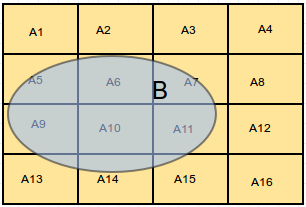
\includegraphics[page=1,scale=0.745]{img/Dvenn2.png}
%\caption{Ejemplo de partición con n=16}
%\end{figure}

%\centerline{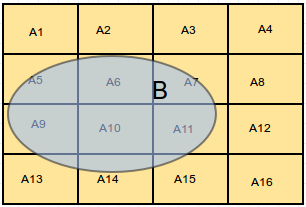
\includegraphics[page=1,scale=0.745]{img/Dvenn2.png}} % scale obtenido empíricamente para que quepa en la página

%\easyimg{img/Dvenn2.png}{El histograma es una aproximación de la función de densidad real en base a la muestra que hemos obtenido.}{lblDensidad}

%\easyimg{img/DensidadAHistograma.png}{El histograma es una aproximación de la función de densidad real en base a la muestra que hemos obtenido.}{lblDensidad}

%\centerline{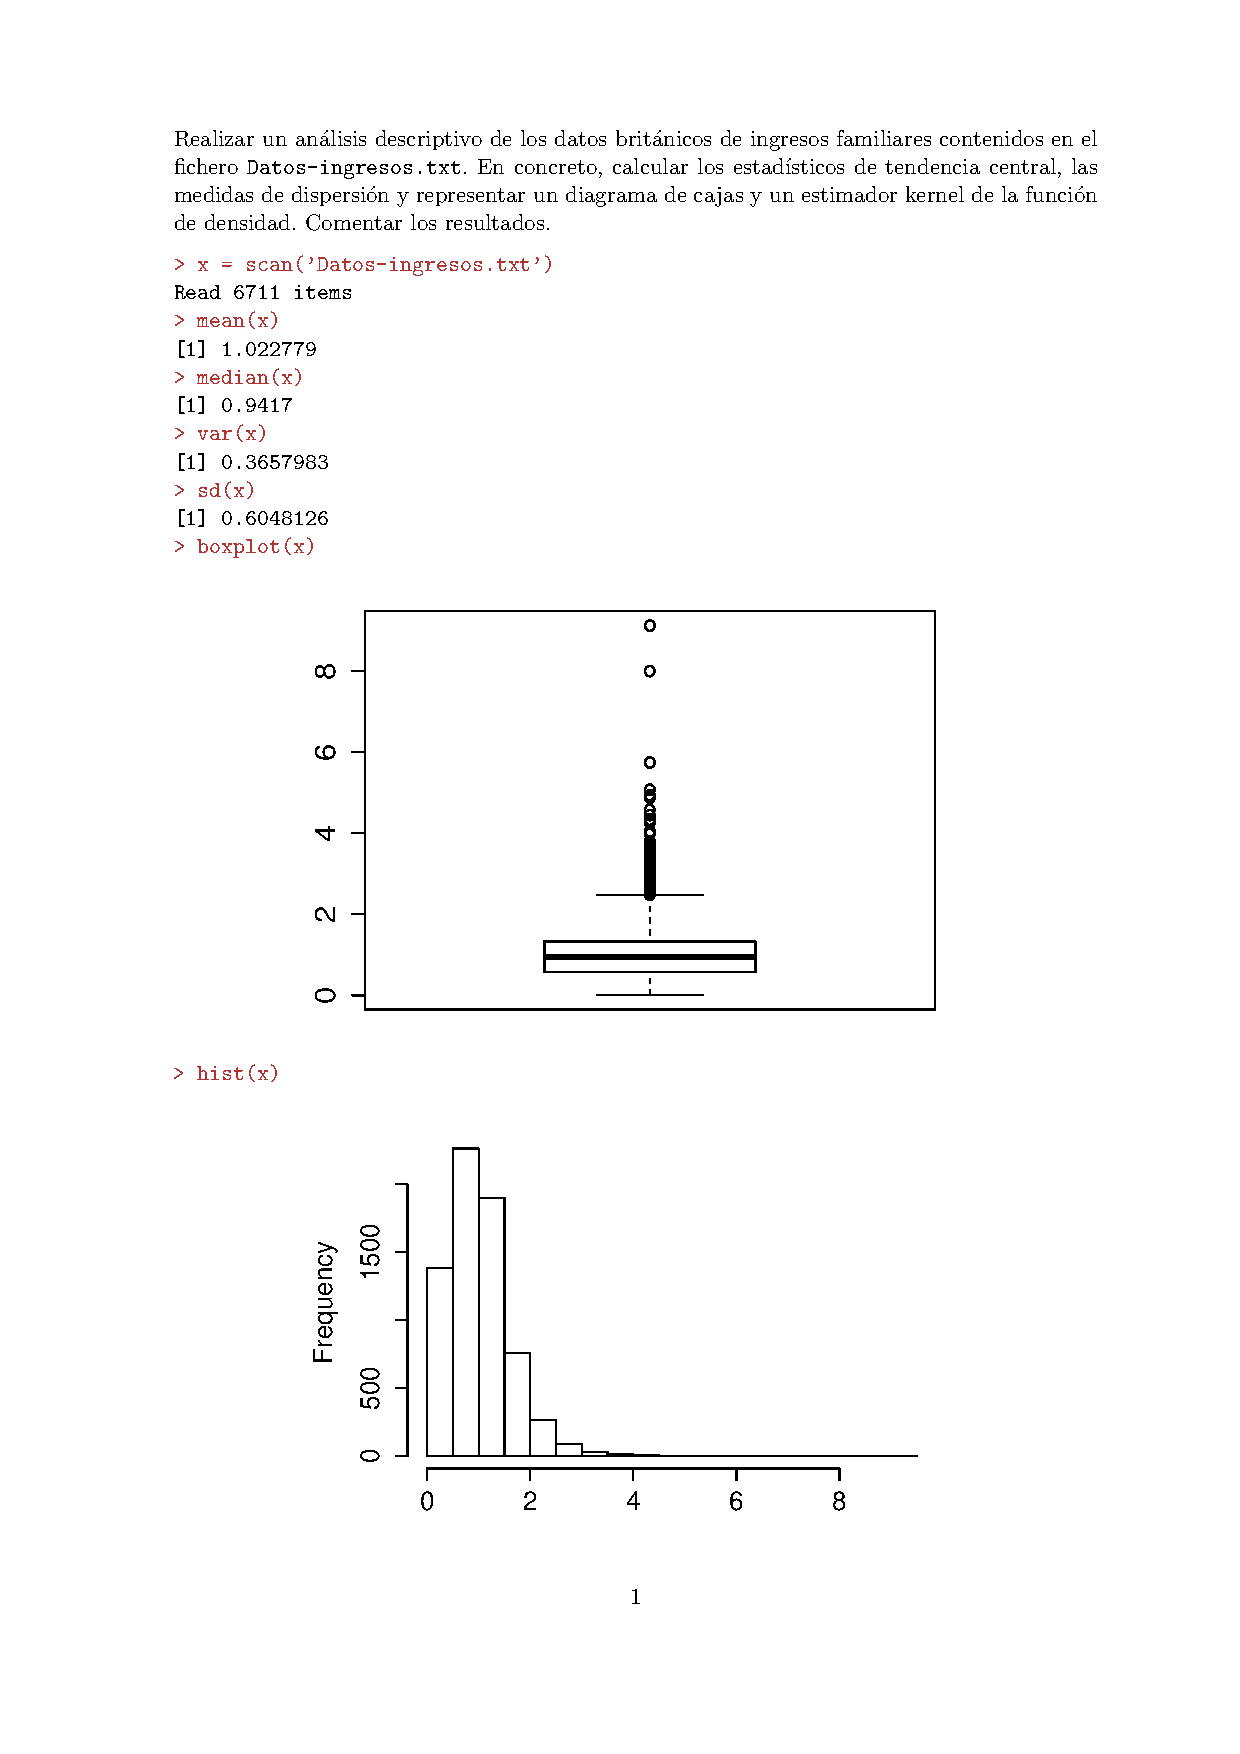
\includegraphics[page=1,scale=0.745]{pdf/_Solucion_T1P1.pdf}} % scale obtenido empíricamente para que quepa en la página


%\includepdf[pages=2-]{pdf/_Solucion_T1P1.pdf}



\chapter{Hojas de Ejercicios}
%
% Soluciones a los ejercicios de Probabilidad II.
%
% Curso 2014 - 2015 2º cuatrimestre
%

%%%%%%%%%%%%%%%%%%%%%%%%%%%%%%%%%%%%%%%%%%%%%%%%%%%%%%%%%%%%%%%%%%%%%%%%%%%%%%%

Todos los ejercicios que así se muestran han sido realizados en primera mano por los alumnos y posteriormente corregidos con las soluciones dadas en clase (Salvo que se indique lo contrario).

Se ha dado prioridad a las soluciones realizadas por el profesor y en algunas ocasiones se han puesto dos soluciones, indicando cuál es la copiada de clase.

Eso no implica que estén exentos de errores :D.

\section{Hoja 1}

\textcolor{blue}{CORREGIDA Y CONTRASTADA CON LAS SOLUCIONES DEL PROFESOR}

Se asume siempre que estamos trabajando en un espacio de probabilidad $(\Omega, \mathcal{A}, P)$, y que  $\mathcal{B}\subset \mathcal{A}$ es una sub-$\sigma$-\'algebra.

%%%%%%%%%%%%%%%%%%  PROBLEMA 1.1  %%%%%%%%%%%%%%%%%%%%%%%%%
\begin{problem}[1]De una urna con 10 bolas blancas y 10 bolas negras se extraen simultaneamente 3 bolas. 
Calcular la probabilidad de que exactamente dos de ellas sean blancas. Responder a la misma
pregunta si las bolas se extraen de manera sucesiva.
\solution

\begin{expla}
En este caso no hay reposición de las bolas extraídas. Por tanto no hay diferencia a la hora de calcular la probabilidad entre la extracción simultánea y la sucesiva.

Para resolver esos problemas, la forma más intuitiva es buscar la fracción:
\[
\frac{\text{Numero de casos favorables}}{\text{Numero de casos posibles}}
\]
\end{expla}
A = Extracción simultánea de 3 bolas blancas

b = blanca

n = negra
\[
P(A)=\underbrace{\frac{10}{20}}_{b}\underbrace{\frac{9}{19}}_{b}\underbrace{\frac{10}{18}}_{n}+\underbrace{\frac{10}{20}}_{b}\underbrace{\frac{10}{19}}_{n}\underbrace{\frac{9}{18}}_{b}+\underbrace{\frac{10}{20}}_{n}\underbrace{\frac{10}{19}}_{b}\underbrace{\frac{9}{18}}_{b} = 3\frac{900}{6840}=\frac{2700}{6840}=0.39
\]

\end{problem}
%%%%%%%%%%%%%%%%%%%%%%%%%%%%%%%%%%%%%%%%%%%%%%%%%%%%%%%%%%


%%%%%%%%%%%%%%%%%%  PROBLEMA 1.2  %%%%%%%%%%%%%%%%%%%%%%%%%
\begin{problem}[2]Disponemos de dos urnas,
$U_1$, que contiene 6 bolas azules y 8 bolas blancas, y
$U_2$,
 que contiene
3 bolas azules y 9 bolas blancas. Se sortea con un dado equilibrado de 4 caras la elecci\'on de una
urna, escogiendose
$U_1$,
si salen 1,
2 o 3, y
$U_2$,
si sale 4. Posteriormente se extrae al azar una bola de
esa urna.

\ppart ?` Cual es la probabilidad de que la bola extraida sea azul?
Sugerencia: usar la regla de la probabilidad total. Respuesta: $43/112$.

\ppart  Si la bola extraida resulta ser blanca  ?`cual es la probabilidad de que proceda de la
urna
$U_1$?

Sugerencia: usar  Bayes o el apartado anterior. Respuesta:
$16/23 = 1 -  43/112$.
\solution
\begin{expla}

$U_1 \rightarrow$ 6a, 8b  (1,2,3)

$U_2 \rightarrow$ 3a, 9b  (4)
\end{expla}
\spart
A = bola extraída azul

$U_1$ = Extraemos de la urna 1

$U_2$ = Extraemos de la urna 2
\[
P(A) = P(A\cap U_1)+P(A\cap U_2) = P(A|U_1)P(U_1)+P(A|U_2)P(U_2)=
\]
\[
=\frac{3}{4}\cdot\frac{6}{14}+\frac{1}{4}\cdot\frac{3}{12}=\frac{18}{56}+\frac{3}{48}=\frac{18}{56}+\frac{1}{16}=\frac{36}{112}+\frac{7}{112}=\frac{43}{112}
\]

\spart
B = bola extraida blanca.

$U_1$ = Extraemos de la urna 1.

\[
P(U_1|B)= \frac{P(U_1 \cap B)}{P(B)} = \frac{P(B|U_1)P(U_1)}{P(B|U_1)P(U_1)+P(B|U_2)P(U_2)}=
\]
\[
=\frac{\frac{8}{14}\cdot\frac{3}{4}}{\frac{8}{14}\cdot\frac{3}{4}+\frac{9}{12}\cdot\frac{1}{4}}=\frac{\frac{24}{56}}{\frac{24}{56}+\frac{9}{48}}=\frac{\frac{24}{56}}{\frac{48}{112}+\frac{21}{112}}=\frac{\frac{24}{56}}{\frac{69}{112}}=\frac{48}{69}=\frac{16}{23}
\]

\end{problem}

%%%%%%%%%%%%%%%%%%%%%%%%%%%%%%%%%%%%%%%%%%%%%%%%%%%%%%%%%%

%%%%%%%%%%%%%%%%%%  PROBLEMA 1.3  %%%%%%%%%%%%%%%%%%%%%%%%%
\begin{problem}[3]Enfermedades raras. Ning\'un test biol\'ogico es 100 $\%$ preciso. Supongamos que un test para
determinar si cierta infecci\'on se ha producido, da falsos positivos en un 1 $\%$ de los casos, y falsos
negativos en un 2 $\%$  de los casos. Si una de cada 100 000 personas entre la poblaci\'on general est\'a
infectada, determinar la probabilidad de que una persona escogida al azar est\'e infectada, sabiendo
que el test ha dado positivo.
\solution

\begin{expla}

\begin{center}
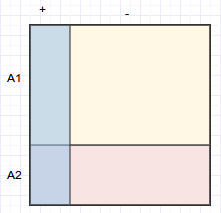
\includegraphics[scale=0.75]{img/Dvenn5.png}
\end{center}


\begin{itemize}

\item Las personas o están infectadas o no están infectadas. 1=P(A1)+P(A2)

\item Los tests o dan positivo o dan negativo: 1 = P(+)+P(-)

\item $A_1$ = persona infectada $\rightarrow P(A1)=10^{-5}$

\item $A_2$ = persona no infectada $\rightarrow P(A_2)=1-10^{-5}$

\item + = test positivo

\item - = test negativo

\item Falso positivo (probabilidad de que el test de positivo estando la persona sin infectar) = $1\% = P(+|A_2)=0.01$

\item $P(+|A_2)+P(-|A_2)=1 \rightarrow P(-|A_2)=0.99$

\item Falso negativo (probabilidad de que el test de negativo sabiendo que la persona esta infectada) = $2\% = P(-|A_1)=0.02$

\item $P(-|A_1)+P(+|A_1)=1 \rightarrow P(+|A_1)=0.98$
\end{itemize}

\end{expla}



\[
P(A_1|+)=\frac{P(A_1\cap +)}{P(+)}=\frac{P(+|A_1)P(A_1)}{P(+|A_1)P(A_1)+P(+|A_2)P(A_2)}=
\]
\[
=\frac{0.98\cdot10^{-5}}{0.98\cdot10^{-5}+0.01\cdot\frac{99999}{10^5}}=0.000979
\]

\end{problem}

%%%%%%%%%%%%%%%%%%%%%%%%%%%%%%%%%%%%%%%%%%%%%%%%%%%%%%%%%%

%%%%%%%%%%%%%%%%%%  PROBLEMA 1.4  %%%%%%%%%%%%%%%%%%%%%%%%%
\begin{problem}[4]Angel y Benito tienen sendas barajas espa\~nolas (40 cartas). Cada uno saca de su
baraja una carta al azar (es decir, con iguales probabilidades, e independientemente). Hallar:

\ppart La probabilidad de obtener al menos un as. 

\ppart La probabilidad de obtener dos cartas del mismo palo. 

\ppart La probabilidad de no obtener ning\'un as.

\ppart La probabilidad de no obtener ni una copa ni una espada.
\solution

\begin{expla}

\end{expla}

\spart
A = obtener al menos un AS

B = no obtener ningun AS
\[
P(A)=\frac{4}{40}\cdot\frac{4}{40}+\frac{4}{40}\cdot\frac{36}{40}+\frac{36}{40}\cdot\frac{4}{40} = 0.19
\]

Otra forma
\[
P(A)=1-P(B)=1-\frac{36}{40}\cdot\frac{36}{40} = 1 - 0.81 = 0.19
\]

\spart
C = dos cartas del mismo palo

Da igual de que palo sea la primera carta, la cosa es que la segunda sea del mismo.

Pensando de otra forma tenemos el siguiente espacio muestral:

$\Omega = \{(c, o),(c, e),(c, b),(c, c),(o, o),(o, c),(o, e),(o, b),(e, c),(e, o),(e, b),(e, e),(b, c),(b, e)\\,(b, o),(b, b)\}$

\[
p(C)=\frac{1}{4}
\]

\spart
B = no obtener ningun AS

\[
P(B)=\frac{36}{40}\cdot\frac{36}{40} = 0.81
\]

\spart
D = no obtener ni una copa ni una espada

\[
P(D) = \frac{20}{40}\cdot\frac{20}{40}=\frac{1}{4}
\]


\end{problem}

%%%%%%%%%%%%%%%%%%%%%%%%%%%%%%%%%%%%%%%%%%%%%%%%%%%%%%%%%%

%%%%%%%%%%%%%%%%%%  PROBLEMA 1.5  %%%%%%%%%%%%%%%%%%%%%%%%%
\begin{problem}[5] Ana y Bea eligen cada una un n\'umero al azar, entre 0 y 2. Sean $A, B, C, D,$ los siguientes
eventos: 

\  $A$: La diferencia entre ambos n\'umeros es al menos 1/3.

\ $B$:   Al menos uno de los n\'umeros es mayor que 1/3.

\ $C$: Los dos n\'umeros son iguales.

\ $D$: El n\'umero de Bea es mayor que 1/3.

Hallar $P(B)$, $P(C)$ y $P(A\cup D)$.
\solution

\begin{expla}
Suponemos que el número elegido es natural, es decir, pertenece al conjunto $\{0,1,2\}$.
\end{expla}

\spart
E = Ningún número es mayor que 1/3.

\[
P(B)=1 - P(E)= 1 - \frac{1}{3}\cdot\frac{1}{3} = \frac{8}{9}
\]

\spart

Da igual qué numero escojas el primero, el que importa es el segundo.

Pensando de otra forma tenemos el siguiente espacio muestral:

$\Omega=\{(0,0),(0,1),(0,2),(1,0),(1,1),(1,2),(2,0),(2,1),(2,2)\}$

\[
P(C)=\frac{1}{3}
\]

\spart
Dado el espacio muestral $\Omega$ definido en el apartado anterior, vemos que:

$P(A)=\frac{2}{3}$ 

Ya que los elementos que cumplen A son: \{(0,1),(0,2),(1,0),(1,2),(2,0),(2,1)\}

$P(D)=\frac{2}{3}$

Ya que los elementos que cumplen D son: \{(0,1),(0,2),(1,1),(1,2),(2,1),(2,2)\}

Por tanto, los elementos que cumplen $A\cup D$ serán la unión de los elementos que cumplen A y los que cumplen D.

\[
P(A \cup D) = \frac{8}{9}
\]

\end{problem}

%%%%%%%%%%%%%%%%%%%%%%%%%%%%%%%%%%%%%%%%%%%%%%%%%%%%%%%%%%

%%%%%%%%%%%%%%%%%%  PROBLEMA 1.6  %%%%%%%%%%%%%%%%%%%%%%%%%
\begin{problem}[6]Con 12 chicas y 4 chicos se forman al azar 4 grupos de 4 personas.
Calcular la probabididad de que haya un chico en cada grupo. Sugerencia:
usar la regla del producto.
 
\solution

\begin{expla}

$A_n$ = Un chico en el grupo n

B = Un chico en cada grupo
\end{expla}

$P(A_1)=4\cdot\frac{4}{16}\cdot\frac{12}{15}\cdot\frac{11}{14}\cdot\frac{10}{13}=0.4835$

$P(A_2|A_1)=4\cdot\frac{3}{12}\cdot\frac{9}{11}\cdot\frac{8}{10}\cdot\frac{7}{9}=0.509$

$P(A_3|A_1\cap A_2)=4\cdot\frac{2}{8}\cdot\frac{6}{7}\cdot\frac{5}{6}\cdot\frac{4}{5}=0.5714$

$P(A_4|A_1\cap A_2\cap A_3)=4\cdot\frac{1}{4}\cdot\frac{3}{3}\cdot\frac{2}{2}\cdot\frac{1}{1}=1$


\[
P(B)=\bigcap_{n=1}^4P(A_n)=P(A_1)P(A_2|A_1)P(A_3|A_2\cap A_1)P(A_4|A_1\cap A_2\cap A_3)=0.14
\]




\end{problem}

%%%%%%%%%%%%%%%%%%%%%%%%%%%%%%%%%%%%%%%%%%%%%%%%%%%%%%%%%%

%%%%%%%%%%%%%%%%%%  PROBLEMA 1.7  %%%%%%%%%%%%%%%%%%%%%%%%%
\begin{problem}[7]Benito tiene un dado  trucado, con 6 caras  numeradas del 1 al 6. 
La probabilidad de las
distintas caras es proporcional al n\'umero de puntos inscritos en
ellas. Hallar la probabilidad de que Benito obtenga con ese dado un n\'umero
par.
\solution

\begin{expla}

Teniendo en cuenta que la suma de los números del dado es 21

\end{expla}

\[
P(par)=P(2)+P(4)+P(6)=\frac{2}{21}+\frac{4}{21}+\frac{6}{21}=\frac{12}{21}=0.57
\]

\end{problem}

%%%%%%%%%%%%%%%%%%%%%%%%%%%%%%%%%%%%%%%%%%%%%%%%%%%%%%%%%%

%%%%%%%%%%%%%%%%%%  PROBLEMA 1.8  %%%%%%%%%%%%%%%%%%%%%%%%%
\begin{problem}[8] En el esquema que aparece a continuaci\'on, el agua fluye  desde $A$ hacia
$B$. Hay, como se indica en el dibujo, ocho compuertas.
Independientemente unas de otras, cada compuerta est\'{a} abierta con
probabilidad $p$, $0 <p <1$. Calcular la probabilidad de que el agua llegue
 de $A$ a $B$. Calcular dicha probabilidad cuando $p = 1/3$.
% Drawing generated by LaTeX-CAD 1.8a - requires latexcad.sty
% (c) 1996 John Leis leis@usq.edu.au
$$\xymatrix{    &   & \circ\ar @{.}[dr]!U||&  &   \circ  \ar @{.}[dr]!U|| &  &  \\
A \ar[r]  & \circ  \ar @{.}[ru]!U||   \ar @{.}[rd]!U||   & &  \circ \ar @{.}[ru]!U||  \ar @{.}[rd]!U||  & & \circ \ar[r]  & B\\  
  &   & \circ \ar @{.}[ru]!U||  &  &   \circ  \ar @{.}[ru]!U||   &  &  }$$ 

Respuestas: $p^8 - 4 p^6 + 4 p^4, 289/6561$.
\solution

\begin{expla}

Se entiende que en las intersecciones el agua va en todas las direcciones.

Llamamos C al punto intermedio (a la intersección entre los dos rombos).

Para llegar hasta el punto C, tenemos que considerar la existencia de 4 puertas: $P_1, P_2, P_3, P_4$, enumeradas de izquierda a derecha y de arriba hacia abajo. Por tanto, para que el agua llegue a C, deben estar abiertas al menos $P_1$ y $P_2$, o $P_3$ y $P_4$.

Si consideramos el siguiente espacio muestral:

$\Omega = \{(0000),(0001),(0010),(0011),(0100),(0101),...,(1110),(1111)\}$

Formado por 16 elementos, en los que un 1 en la posición n indica que la puerta $P_n$ está abierta, tenemos que con esas 16 combinaciones el agua NO llegaría a C en los elementos con 4 0's (1), los elementos con 3 0,s (4) y los elementos 1010, 0101, 1001, 0110 (4). Por tanto solo nos sirven 7 combinaciones. La de todo 1's, las de 3 1's (4), 1100 y 0011.

$P(1100)=P(0011)=p^2(1-p)^2$

$P(1110)=P(1101)=P(1011)=P(0111)=p^3(1-p)$

$P(1111)=p^4$

Por tanto la probabilidad de llegar a C desde A es:

\[
P(AC)=2p^2(1-p)^2+4p^3(1-p)+p^4
\]

La probabilidad de llegar al punto B, desde el punto C es exactamente la misma que la de ir desde A hasta C.
\end{expla}
Por tanto, según la regla del producto quedaría:
\[
P(AB)=P(AC)P(CB|AC)=P(AC)^2=(2p^2(1-p)^2+4p^3(1-p)+p^4)^2=
\]
\[
=(2p^2(p^2+1-2p)+4p^3-4p^4+p^4)^2 = (2p^4 + 2p^2-4p^3-3p^4+4p^3)^2 =
\]
\[
=(-p^4+2p^2)^2=p^8-4p^6+4p^4
\]

Para $p=\frac{1}{3}$, nos queda:

\[
P(AB)=\frac{1}{3^8}-4\cdot\frac{1}{3^6}+4\cdot\frac{1}{3^4}=\frac{289}{6561}
\]



\end{problem}

%%%%%%%%%%%%%%%%%%%%%%%%%%%%%%%%%%%%%%%%%%%%%%%%%%%%%%%%%%

%%%%%%%%%%%%%%%%%%  PROBLEMA 1.9  %%%%%%%%%%%%%%%%%%%%%%%%%
\begin{problem}[9]En una reuni\'on hay 25 personas. Calcular la
probabilidad de que celebren su cumplea\~{n}os el mismo d\'ia del
a\~{n}o al menos dos personas. Observación: con frecuencia es m\'as f\'acil
calcular intersecciones que uniones. Sugerencia: calcular la probabilidad
del evento complementario.
\solution


A = cumpleaños mismo día al menos dos personas.

$A^c$ = cumpleaños distinto día todas las personas.

\[
P(A)=1-P(A^c)=1-\frac{365}{365}\cdot\frac{364}{365}\cdot\frac{363}{365}\cdot...\cdot\frac{341}{365}=1-0.43=0.57
\]

\end{problem}

%%%%%%%%%%%%%%%%%%%%%%%%%%%%%%%%%%%%%%%%%%%%%%%%%%%%%%%%%%

%%%%%%%%%%%%%%%%%%  PROBLEMA 1.10  %%%%%%%%%%%%%%%%%%%%%%%%%
\begin{problem}[10]Inclusi\'on-Exclusi\'on: Probar que 
$
P(\cup_{i=1}^n A_i)= \sum_{k=1}^n \sum_{I\subset \{1, \dots, n\}, |I| = k} (-1)^{k-1}
P(\cap_{i\in I} A_i).
$
\solution

\begin{expla}

Tenemos que probar:

\[
P(\bigcup_{i=1}^nA_i)=\sum_{k=1}^{n}\sum_{I\subset \{1,...,n\}:|I|=k}(-1)^{k-1}P(\bigcap_{i\in I}A_i)
\]

Vamos a ver lo que significa para una colección de 3 subconjuntos $\{A_1,A_2,A_3\}$; de forma que sea fácil de ver. El término que puede llevar a la duda es el segundo sumatorio, sólo dice que escojamos todas las subcolecciones posibles de tamaño k dentro de nuestra colección $\{A_1,A_2,A_3\}$.

\begin{center}
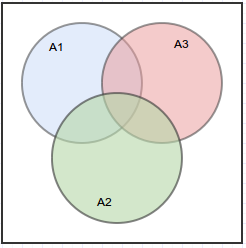
\includegraphics[scale=0.75]{img/Dvenn4.png}
\end{center}

\[
P(A_1\cup A_2 \cup A_3)=\underbrace{(-1)^0P(A_1)+(-1)^0P(A_2)+(-1)^0P(A_3)}_{k=1}+
\]
\[
+\underbrace{(-1)^1P(A_1\cap A_2)+(-1)^1P(A_1\cap A_3)+(-1)^1P(A_2\cap A_3)}_{k=2}+\underbrace{(-1)^2P(A_1\cap A_2\cap A_3)}_{k=3}=
\]
\[
=\underbrace{P(A_1)+P(A_2)+P(A_3)}_{k=1}+\underbrace{(-P(A_1\cap A_2)-P(A_1\cap A_3)-P(A_2\cap A_3))}_{k=2}+\underbrace{P(A_1\cap A_2\cap A_3)}_{k=3}
\]

\end{expla}

\begin{itemize}
        \item Hipótesis:

        Suponemos que \[
        P(\bigcup_{i=1}^nA_i)=\sum_{k=1}^{n}\sum_{I\subset
\{1,...,n\}:|I|=k}(-1)^{k-1}P(\bigcap_{i\in I}A_i)
        \]
        \item Base de inducción: n=2

        Para n = 2 se tiene que $$P(A_1\cup A_2)=P(A_1)+P(A_2)-P(A_1\cap
A_2)$$ Vemos que esto es cierto para cualquier conjunto.

        \item Inducción:
        Supongamos la hipótesis cierta para n. Vamos a demostrar que es
válida para n+1.
        $${P\big(\bigcup_{i=1}^{n+1}A_i\big)=P\big((\bigcup_{i=1}^nA_i)\cup A_{n+1}\big)=P\big(\bigcup_{i=1}^nA_i\big)+P(A_{n+1})-P\big((\bigcup_{i=1}^nA_i)\cap
A_{n+1}\big)}$$
        A esto hemos llegado aplicando la fórmula para n = 2.

        Por hipótesis inductiva sabemos lo que vale $P\big(\bigcup_{i=1}^nA_i\big)$.
        Ahora escribimos $P\big((\bigcup_{i=1}^nA_i)\cap
A_{n+1}\big)=P\big(\bigcup_{i=1}^n(A_i\cap A_{n+1})\big)$

        $$P(\bigcup_{i=1}^n(A_i\cap A_{n+1}))=\sum_{1\leq i_1\leq
n}P(A_{i_1}\cap A_{n+1})\quad -\sum_{1\leq i_1<i_2\leq
n}P\big((A_{i_1}\cap A_{n+1})\cap (A_{i_2}\cap A_{n+1})\big)\quad
$$$$+\sum_{1\leq i_1<i_2<i_3\leq n}P\big((A_{i_1}\cap A_{n+1})\cap
(A_{i_2}\cap A_{n+1})\cap (A_{i_3}\cap
A_{n+1})\big)\;+\;\cdots$$$$+\;(-1)^{n-1}\sum_{1\leq
i_1<\cdots<i_n\leq n}P\big((A_{i_1}\cap A_{n+1})\cap \cdots \cap
(A_{i_n}\cap A_{n+1})\big)$$

        Además tenemos que:
        $$ P\big((A_{i_1}\cap A_{n+1})\cap(A_{i_2}\cap A_{n+1})\cap \cdots
\cap (A_{i_n}\cap A_{n+1})\big)=P(A_{i_1}\cap A_{i_2}\cap\cdots\cap
A_{i_n}\cap A_{n+1})$$
        Al final nos queda que :
        $$P(\bigcup_{i=1}^{n+1}A_i) = \sum_{k=1}^{n}\sum_{I\subset
\{1,...,n\}:|I|=k}(-1)^{k-1}P(\bigcap_{i\in I}A_i) + P(A_{n+1})$$$$ -
\sum_{k=1}^{n}\sum_{I\subset \{1,...,n\}:|I|=k}(-1)^{k-1}P(A_{i_1}
\cap A_{i_2} \cap .... \cap A_{i_k} \cap A_{n+1})$$
        Y esto es igual a:
        $$\sum_{k=1}^{n+1}\sum_{I\subset
\{1,...,n+1\}:|I|=k}(-1)^{k-1}P(\bigcap_{i\in I}A_i)$$
\end{itemize}

\end{problem}

%%%%%%%%%%%%%%%%%%%%%%%%%%%%%%%%%%%%%%%%%%%%%%%%%%%%%%%%%%

%%%%%%%%%%%%%%%%%%  PROBLEMA 1.11  %%%%%%%%%%%%%%%%%%%%%%%%%
\begin{problem}[11] Emparejamientos al azar: tenemos $n$ cartas, que colocamos al azar en $n$ sobres
(en vez de cuidadosamente poner cada carta en su sobre).
Calcular la probabilidad de que alguna carta est\'a en el sobre correcto
(es decir, al menos una carta). Estimar dicha probabilidad cuando
$n\to\infty$. Sugerencia: usar Inclusi\'on-Exclusi\'on.
Observar que la probabilidad de que todas las cartas de 1 a $k$ esten en el sobre correcto
es $(n-k)!/n!$. Respuesta en el l\'{\i}mite: $1 - e^{-1}$.
\solution

\begin{expla}

Para hacernos una idea del problema consideramos n=3 y el siguiente espacio de probabilidad:

$\Omega_3=\{(123),(132),(213),(231),(312),(321)\}$

Que representa todas las posibles combinaciones (numero de carta-numero sobre, es decir, 3!) que puede haber con 3 cartas y 3 sobres. 

Según esto la probabilidad de que la carta 1 este en el sobre 1 sería: $\frac{2}{6} = \frac{2}{3\cdot 2}=\frac{1}{3}$

Sea: $A_i$ = carta n-esima en el sobre correcto.

Se observa fácilmente que: $P(A_i) = \frac{(n-1)!}{n!}$, siendo n el número de cartas totales.

Sea A = todas las cartas en el sobre correcto. Simplemente hay que observar que si la primera carta esta en el sobre correcto, para poner la segunda en su sobre tenemos una carta y un sobre menos donde elegir.

\[
P(A)=P(\bigcap_{j=1}^nA_j)=P(A_1)P(A_2|A_1)P(A_3|A_2\cap A_1)...P(A_j|\bigcap_{i=1}^{n-1}A_i)=
\]
\[
\frac{(n-1)!}{n!}\cdot\frac{(n-2)!}{(n-1)!}\cdot\frac{(n-3)!}{(n-2)!}\cdot...\cdot\frac{(n-n+1)!}{(n-n+2)!}\cdot\frac{(n-n)!}{(n-n+1)!}=\frac{1}{n!}
\]

Sea $B_k$ = todas las cartas de la 1 a la k en el sobre correcto.

\[
P(B_k)=P(\bigcap_{n=1}^kA_n)=P(A_1)P(A_2|A_1)P(A_3|A_2\cap A_1)...P(A_n|\bigcap_{i=1}^{k-1}A_i)=
\]
\[
\frac{(n-1)!}{n!}\cdot\frac{(n-2)!}{(n-1)!}\cdot\frac{(n-3)!}{(n-2)!}\cdot...\cdot\frac{(n-k+1)!}{(n-k+2)!}\cdot\frac{(n-k)!}{(n-k+1)!}=\frac{(n-k)!}{n!}
\]

Esta probabilidad es la misma cojamos las k primeras cartas o k cartas en diferentes posiciones.
\end{expla}

Vamos a usar Inclusión-Exclusión:
\[
P(\bigcup_{i=1}^nA_i)=\sum_{k=1}^{n}\sum_{I\subset \{1,...,n\}:|I|=k}(-1)^{k-1}P(\bigcap_{i\in I}A_i)
\]

C = Al menos una carta en el sobre correcto: 

\[
P(C)=P(\bigcup_{i=1}^nA_i)=\sum_{k=1}^{n}\sum_{I\subset \{1,...,n\}:|I|=k}(-1)^{k-1}\frac{(n-k)!}{n!}=\sum_{k=1}^{n}\left( (-1)^{k-1}\frac{(n-k)!}{n!}\binom{n}{k}\right)=
\]
\[
= \sum_{k=1}^{n}\left( (-1)^{k-1}\frac{(n-k)!}{n!}\cdot \frac{n!}{(n-k)!\cdot k!}\right)= \sum_{k=1}^{n}\left( (-1)^{k-1}\frac{1}{k!}\right) \stackrel{n \rightarrow \infty}{\rightarrow} 1-e^{-1}
\]
Ahora vamos a demostrar que:

\[
\sum_{k=1}^{n}\left( (-1)^{k-1}\frac{1}{k!}\right) \stackrel{n \rightarrow \infty}{\rightarrow} 1-e^{-1}
\]

\begin{proof}
\[
\sum_{k=1}^{n}\left( (-1)^{k-1}\frac{1}{k!}\right) = 1 + \sum_{k=0}^{n}\left((-1)^{k-1}\frac{1}{k!}\right) = 1 - \sum_{k=0}^{n}\left((-1)^{k}\frac{1}{k!}\right)
\]

Por otro lado, aplicando Taylor, sabemos que:

\[
f(x)=e^x=f(0)+\frac{f'(0)}{1!}(x-0)+\frac{f''(0)}{2!}(x-0)^2...
\]

Y por tanto:

\[
f(-1)=e^{-1}=1-\frac{1}{1!}+\frac{1}{2!}-\frac{1}{3!}... = \sum_{k=0}^{n}\left((-1)^{k}\frac{1}{k!}\right)
\]
\end{proof}



\end{problem}

%%%%%%%%%%%%%%%%%%%%%%%%%%%%%%%%%%%%%%%%%%%%%%%%%%%%%%%%%%

%%%%%%%%%%%%%%%%%%  PROBLEMA 1.12  %%%%%%%%%%%%%%%%%%%%%%%%%
\begin{problem}[12] Media o esperanza. Con los datos del problema anterior, calcular el n\'umero esperado de
emparejamientos al azar, es decir, cuantas cartas esperamos que est\'an en el sobre correcto.
Comentario: este problema es muy f\'acil.
\solution

\begin{expla}
\[
\mathbb{E}(X) = \sum_{w \in \Omega} X(w)P(w)
\]

En nuestro caso $\Omega$ esta formado por n! eventos (tal y como vimos en el ejercicio anterior), X es una variable aleatoria que vale "m", siendo m el número de cartas que están bien emparejadas con su sobre.

Así no se debe hacer: 
Llamamos $P(B_k)$ a la probabilidad de k cartas bien emparejadas. 

\[
\mathbb{E}(X) = \sum_{w \in \Omega} X(w)P(w) = \sum_{k=0}^n kP(B_k) = \sum_{k=0}^n k\cdot\frac{(n-k)!}{n!}
\]

Pero esto no vale porque $P(B_k)$ no te específica si el resto de cartas están o no emparejadas.
\end{expla}
Llamamos $A$ a la variable aleatoria que dice cuántas cartas están en el sobre correcto.

Consideramos $A_i$ a la variable aleatoria que vale 1 si la carta i está en el sobre i-ésimo y 0 en caso contrario. Y tenemos que $P(A_i=1)=\frac{1}{n}$.

Por tanto:
\[
\mathbb{E}(A)=\mathbb{E}({\sum_{i=1}^{n} A_i}) = \sum_{i=1}^n \mathbb{E}(A_i) = \sum_{i=1}^n 1 \cdot \frac{1}{n} = 1
\]




\end{problem}

%%%%%%%%%%%%%%%%%%%%%%%%%%%%%%%%%%%%%%%%%%%%%%%%%%%%%%%%%%

%%%%%%%%%%%%%%%%%%  PROBLEMA 1.13  %%%%%%%%%%%%%%%%%%%%%%%%%
\begin{problem}[13] Dado $C$ con $P(C) > 0$, decimos que $A$ y $B$ son condicionalmente independientes
con respecto a $C$ si $P(A\cap B|C) =P(A|C) P(B|C)$. Probar que si  $P(B\cap C) > 0$, 
$P(A\cap B|C) =P(A|C) P(B|C)$ es equivalente a $P(A|C) = P(A|B \cap C)$. 


\solution

\begin{expla}
Partimos de: $P(A\cap B|C)=P(A|C)P(B|C)$  

Despejamos $P(A|C)$ y operamos:
\end{expla}

\[
P(A|C)=\frac{P(A\cap B|C)}{P(B|C)}=\frac{\frac{P(A\cap B\cap C)}{P(C)}}{\frac{P(B \cap C)}{P(C)}}=\frac{P(A \cap B\cap C)}{P(B\cap C)}=P(A|B\cap C)
\]

\end{problem}

%%%%%%%%%%%%%%%%%%%%%%%%%%%%%%%%%%%%%%%%%%%%%%%%%%%%%%%%%%

%%%%%%%%%%%%%%%%%%  PROBLEMA 1.14  %%%%%%%%%%%%%%%%%%%%%%%%%
\begin{problem}[14] Estudiar para $ \alpha>0 $ la convergencia en
media cuadr\'atica (es decir, en $L^2$) de la sucesi\'on $\{X_n\}_{n=1}^\infty$, sabiendo que

\[  P(X_n=n)=\frac{1}{n^\alpha}, \hspace{5mm} P(X_n=0)=1-\frac{1}{n^\alpha}.
  \]
\solution

\begin{expla}
Dado un espacio de probabilidad $(\Omega, \algb{M}, P)$, y una variable aleatoria $X_n$, tenemos que $X_n$ es también una función medible que cumple:

\[
X_n \stackrel{L_2 (n\rightarrow \infty)}{\rightarrow} X \Leftrightarrow \norm{X_n -X}_2  \rightarrow 0 \Leftrightarrow \int{\abs{X_n -X}^2dP} \rightarrow 0
\]

Tenemos que cuando $n \rightarrow \infty$, se cumple que:
\begin{itemize}
\item $P(X_n = n) \rightarrow 0$
\item $P(X_n = 0) \rightarrow 1$
\end{itemize}

Así definimos X como una variable aleatoria que cumple:

\begin{itemize}
\item $P(X = n) = 0$
\item $P(X = 0) = 1$
\end{itemize}

\end{expla}

\[
\int{\abs{X_n -X}^2dP} = \int_{\Omega}{\abs{X_n(w) -X(w)}^2dP(w)}
\]

Como X toma el valor 0 con probabilidad 1, tenemos:

\[
\int_{\Omega}\abs{X_n(w) -X(w)}^2dP(w)=\int_{\Omega}\abs{X_n(w)}^2dP(w)=\int_{\Omega}(X_n(w))^2dP(w) =
\]
\[
=\mathbb{E}((X_n)^2)=n^2\cdot\frac{1}{n^{\alpha}}+0^2\cdot(1-\frac{1}{n^{\alpha}})=\frac{n^2}{n^{\alpha}} \stackrel{n \rightarrow \infty}{\rightarrow} 0 \text{ si } \alpha>2 
\]

Por tanto la sucesión $\{X_n\}_{n=1}^\infty$ converge cuadráticamente si $\alpha > 2$.



\end{problem}

%%%%%%%%%%%%%%%%%%%%%%%%%%%%%%%%%%%%%%%%%%%%%%%%%%%%%%%%%%





\newpage
\section{Hoja 2}

\textcolor{blue}{CORREGIDA Y CONTRASTADA CON LAS SOLUCIONES DEL PROFESOR}

Se asume siempre que estamos trabajando en un espacio de probabilidad $(\Omega, \mathcal{A}, P)$,
y que  $\mathcal{B}\subset \mathcal{A}$ es una sub-$\sigma$-\'algebra.


%%%%%%%%%%%%%%%%%%  PROBLEMA 2.1  %%%%%%%%%%%%%%%%%%%%%%%%%
\begin{problem}[1]Sea $X$ una v.a. con distribuci\'on $N(0,1)$ (normal con media 0 y varianza 1). 
Calcular el tercer momento $E(X^3)$.
\solution

\begin{expla}
Sea una variable aleatoria X, a esta se le asigna una función de distribución ($F_X(t)$) y otra de densidad ($f_X(t)$) que cumplen:

\[
F_X(t)=\int_{-\infty}^{t}f_x(t)dt
\]

En el caso de distribución N(0,1) tenemos:
\[
f(x)=\frac{e^{-t^2/2}}{\sqrt{2\pi}}
\]

Sabiendo que la esperanza se calcula como:
\[
\mathbb{E}(X)=\int_{-\infty}^{\infty}t\cdot f(t)dt
\]

Escribimos:
\end{expla}

\[
\mathbb{E}(X^3)=\int_{-\infty}^{\infty}t^3\cdot \frac{e^{-t^2/2}}{\sqrt{2\pi}}dt = \frac{1}{\sqrt{2\pi}}\int_{-\infty}^{\infty}t^3\cdot e^{-t^2/2}dt
\]

Hacemos un cambio de variable y llamamos $w=\frac{t^2}{2}$ por tanto: $\frac{dw}{dt}=t$

\[
\frac{1}{\sqrt{2\pi}}\int t^3\cdot e^{-t^2/2}dt = \frac{1}{\sqrt{2\pi}}\int 2tw\cdot e^{-w}\frac{dw}{t} = \frac{2}{\sqrt{2\pi}}\int w\cdot e^{-w}dw
\]

Ahora vamos a integrar por partes

$u=w$

$du=1$

$v=-e^{-w}$

$dv=e^{-w}$

\[
\frac{2}{\sqrt{2\pi}}\int w\cdot e^{-w}dw = \frac{2}{\sqrt{2\pi}}\left( -we^{-w}+\int e^{-w}dw \right) =\frac{2}{\sqrt{2\pi}}\left( -we^{-w}-e^{-w} \right)=
\]
\[
= \frac{-2e^{-w}}{\sqrt{2\pi}}(w+1)
\]

Y nos queda que:
\[
\mathbb{E}(X^3)=\int_{-\infty}^{\infty}t^3\cdot \frac{e^{-t^2/2}}{\sqrt{2\pi}}dt = \left.\frac{-2e^{-t^2/2}}{\sqrt{2\pi}}(t^2/2+1)\right|_{-\infty}^{\infty}=0
\]




\end{problem}
%%%%%%%%%%%%%%%%%%%%%%%%%%%%%%%%%%%%%%%%%%%%%%%%%%%%%%%%%%


%%%%%%%%%%%%%%%%%%  PROBLEMA 2.2  %%%%%%%%%%%%%%%%%%%%%%%%%
\begin{problem}[2]Sea $\mathcal{B} \subset \mathcal{A}$ la sub-$\sigma$-\'algebra generada por una partici\'on
$\{A_1, \dots,A_n\}$ de $\Omega$, donde todos los conjuntos de la partici\'on tienen probabilidad positiva.
Dada una v.a. $X$, demostrar que si la variable aleatoria $T(X)$ satisface

1) para todo $B\in \mathcal{B}$, $\int_B T(X) dP = \int_B X dP$, y

2) $T(X)$ es  $\mathcal{B}$-medible, 

entonces cuando $w\in A_i$, $T(X)(w)= \frac{1}{P(A_i)}\int_{A_i} X dP$.

Probar que si  $T(X)(w)$ est\'a definida mediante  $T(X)(w):= \frac{1}{P(A_i)}\int_{A_i} X dP$ cuando  
 $w\in A_i$, entonces $T(X)$ satisface las condiciones 1) y 2) enunciadas arriba.

Este ejercicio demuestra que las condiciones 1) y 2) determinan de modo \'unico la esperanza condicional,
cuando la  sub-$\sigma$-\'algebra est\'a generada por una partici\'on (el resultado tambi\'en es cierto
para  sub-$\sigma$-\'algebras arbitrarias, pero entonces es necesario definir la esperanza condicional
mediante un procedimiento distinto).
\solution

\begin{expla}

Tenemos que demostrar la doble implicación, empezamos de izquierda a derecha y luego lo demostraremos de derecha a izquierda.
\end{expla}

\begin{itemize}
\item $\Rightarrow)$ Sabemos que:
\begin{enumerate}
\item $\forall B \in \algb{B}, \int_{B}T(X)dP = \int_{B}XdP$
\item $T(X)$ es $\algb{B}-medible$
\end{enumerate}

Tenemos que llegar a: $T(X)(w)= \frac{1}{P(A_i)}\int_{A_i} X dP$ con $w \in A_i$.

Partimos del punto 1, sabemos que esa propiedad se cumple $\forall B \in \algb{B}$, por tanto, se cumplirá para todos los elementos $A_i$ de la partición:
\[
\int_{A_i}T(X)dP = \int_{A_i}XdP  \Leftrightarrow  \frac{1}{P(A_i)}\cdot\int_{A_i}T(X)dP = \frac{1}{P(A_i)}\cdot\int_{A_i}XdP
\]

la parte derecha ya es idéntica a la parte derecha de la fórmula a la que queremos llegar, por tanto, sólo nos queda demostrar que: $\frac{1}{P(A_i)}\cdot\int_{A_i}T(X)dP = T(X)(w)$

Observamos que esto es cierto si la integral no depende de T(X) y se puede sacar como constante, ya que de darse eso tendríamos:

\[
\frac{1}{P(A_i)}\cdot\int_{A_i}T(X)dP = \frac{1}{P(A_i)}\cdot T(X)\cdot\int_{A_i}1dP = \frac{P(A_i) \cdot T(X)}{P(A_i)} = T(X)
\]

(Ver definición de integral sobre una medida)

Es aquí cuando usamos que T(X) es $\algb{B}-medible$. Eso quiere decir, que la antiimagen de un medible pertenece a $\algb{B}$. Como los elementos de $\algb{B}$ son los conjuntos $A_i$, quiere decir que T(X) (que es lo mismo que T(X(w))) tiene que tener valor constante para todos los elementos $w \in A_i$. 

¿Por qué?, bueno, piensa que en $A_2$ tenemos 2 elementos: $w_1$ y $w_2$, si $T(X(w_1))=2$ y $T(X(w_2))=4$, entonces, $T^{-1}(1,3)=w_1$ que es un elemento que NO pertenece a $\algb{B}$. Si no ha quedado claro con esta explicación, se puede ver algún ejemplo más tras la demostración de 'Ley de X' de estos apuntes.

Por tanto, definimos T(X)(w)=T(X(w)) y concluimos que T(X)(w) es constante para los w pertenecientes a cada partición $A_i$. Por tanto queda demostrada la implicación primera ya que:

\[
\frac{1}{P(A_i)}\cdot\int_{A_i}T(X)(w)dP = \frac{1}{P(A_i)}\cdot T(X)(w)\cdot\int_{A_i}1dP = \frac{P(A_i) \cdot T(X)(w)}{P(A_i)} =
\]
\[
=T(X)(w)  \text{ para todo } w \in A_i
\]

\item $\Leftarrow)$ Sabemos que:

$T(X)(w)= \frac{1}{P(A_i)}\int_{A_i} X dP$ con $w \in A_i$.

Tenemos que llegar a: 
\begin{enumerate}
\item $\forall B \in \algb{B}, \int_{B}T(X)dP = \int_{B}XdP$
\item $T(X)$ es $\algb{B}$-medible
\end{enumerate}

Empezamos demostrando 2: Lo hacemos por reducción al absurdo. Suponemos que no es $\algb{B}$-medible, entonces existe al menos un conjunto $A_j$ con al menos dos elementos $w_1$ y $w_2$ tal que $T(X(w_1))=c_1$ y $T(X(w_2))=c_2$ con $c_1 \neq c_2$. Por tanto:

\[
c_1=T(X)(w_1)=\frac{1}{P(A_j)}\int_{A_j} X dP \neq \frac{1}{P(A_j)}\int_{A_j} X dP=T(X)(w_2)=c_2
\]

Lo cual es contradictorio, porque como podemos ver, T(X)(w) es constante para elementos pertenecientes al mismo $A_i$, es decir, a la misma clase de equivalencia.

Ahora demostramos 1:

\[
T(X)(w)= \frac{1}{P(A_i)}\int_{A_i}X dP \Leftrightarrow T(X)(w)\cdot P(A_i)= \int_{A_i}X dP
\]

Como T(X) es $\algb{B}$-medible, entonces es constante para todos los w pertenecientes a una misma clase de equivalencia $A_i$, por tanto podemos introducir T(X) dentro de la integral quedando:
\[
\int_{A_i}T(X)dP = \int_{A_i}XdP
\]

Sea $B \in \algb{B}$ de modo que $B=A_{i_1} \cup A_{i_2} \cup ... \cup A_{i_k}$, entonces llegamos a la propiedad 1:

\[
\forall B \in \algb{B}, \int_{B}T(X)dP = \int_{A_{i_1}}T(X)dP + \int_{A_{i_2}}T(X)dP + ... + \int_{A_{i_k}}T(X)dP =
\]
\[
= \int_{A_{i_1}}XdP + \int_{A_{i_2}}XdP + ... + \int_{A_{i_k}}XdP = \int_{B}XdP
\]



\end{itemize}




\end{problem}

%%%%%%%%%%%%%%%%%%%%%%%%%%%%%%%%%%%%%%%%%%%%%%%%%%%%%%%%%%

%%%%%%%%%%%%%%%%%%  PROBLEMA 2.3  %%%%%%%%%%%%%%%%%%%%%%%%%
\begin{problem}[3]En un examen tipo test se plantean 5 preguntas para responder verdadero o falso. 
 Los puntos asignados a las preguntas V o F son: respuesta correcta,
1 punto, respuesta incorrecta,
- 1 punto, en blanco, 0 puntos. Valor m\'{\i}nimo del  problema: 0 puntos. Es decir, si la puntuaci\'on es
negativa se asigna un cero al problema. 

a)  Calcular la nota esperada de un alumno que responda a las 5 perguntas
de manera aleatoria, por ejemplo lanzando una moneda equilibrada 5 veces.

b) Sabiendo que el  alumno ha respondido correctamente a  la
primera pregunta, calcular la nota esperada.
\solution

\textcolor{green}{ESTA SOLUCIONADO EN EL EXAMEN FINAL DEL CURSO 2013/2014}

\begin{expla}
Se nos podría ocurrir plantear el problema de la siguiente manera:

Sea $X_i$ v.a. independientes que cumplen : $P(X_i(w)=1)=1/2=P(X_i(w)=-1) \forall i$

Por tanto, tenemos que:
\[
\mathbb{E}(X_i)=\frac{1}{2}\cdot(1)+\frac{1}{2}\cdot(-1)=0
\] 

Y si consideramos que i=5:
\[
\mathbb{E}\left(\sum_{i=1}^{5}X_i\right)=\sum_{i=1}^{5}\mathbb{E}(X_i)=0
\]

Pero esto no lo podemos plantear así ya que la nota mínima del problema es de 0. Y eso implica que las variables aleatorias $X_i$ no se pueden sumar ya que son dependientes y no expresarían la solución del problema.

Por tanto lo planteamos de otra manera: Sea el siguiente espacio muestral:

$\Omega = \{(00000), (00001), (00010),..., (11111)\}$, hay un total de $2^5=32$ combinaciones diferentes de posibles respuestas. Teniendo en cuenta que las preguntas no se dejan en blanco. Consideramos la variable aleatoria Z, asociada a ese espacio muestral.

\end{expla}

\spart
\begin{itemize}
\item 5 mal: nota del problema = 0
\item 1 bien y 4 mal: nota del problema = 0
\item 2 bien y 3 mal: nota del problema = 0
\item 3 bien y 2 mal: nota del problema = 1
\item 4 bien y 1 mal: nota del problema = 3
\item 5 bien: nota del problema = 5
\end{itemize}

\[
\mathbb{E}(Z)=\frac{\binom{5}{0}}{32}\cdot0+\frac{\binom{5}{1}}{32}\cdot0+\frac{\binom{5}{2}}{32}\cdot0+\frac{\binom{5}{3}}{32}\cdot1+\frac{\binom{5}{4}}{32}\cdot3+\frac{\binom{5}{5}}{32}\cdot5=
\]
\[
=\frac{\binom{5}{3}}{32}\cdot1+\frac{\binom{5}{4}}{32}\cdot3+\frac{\binom{5}{5}}{32}\cdot5=\frac{\frac{5!}{3!\cdot 2!}}{32}\cdot1+\frac{\frac{5!}{4!\cdot 1!}}{32}\cdot3+\frac{1}{32}\cdot5=\frac{10}{32}\cdot1+\frac{5}{32}\cdot3+\frac{1}{32}\cdot5=\frac{10}{32}+\frac{15}{32}+\frac{5}{32}=\frac{30}{32}=0.9375
\]

\spart
En esta ocasión:

A = posibles respuestas sabiendo que la primera respuesta es correcta =$\{(10000), (10001), (10010),..., (11111)\}$.


Estudiamos las posibles dentro del conjunto A, mirando los 4 digitos de mas a la derecha:
\begin{itemize}
\item 4 mal: nota del problema = 0
\item 1 bien y 3 mal: nota del problema = 0
\item 2 bien y 2 mal: nota del problema = 1
\item 3 bien y 1 mal: nota del problema = 3
\item 4 bien: nota del problema = 5
\end{itemize}

\[
\mathbb{E}(Z|A)=\frac{1}{P(A)}\left( \frac{\binom{4}{0}}{32}\cdot0+\frac{\binom{4}{1}}{32}\cdot0+\frac{\binom{4}{2}}{32}\cdot1+\frac{\binom{4}{3}}{32}\cdot3+\frac{\binom{4}{4}}{32}\cdot5 \right)=
\]

\[
= \frac{1}{\frac{1}{2}}\left( \frac{\binom{4}{2}}{32}\cdot1+\frac{\binom{4}{3}}{32}\cdot3+\frac{\binom{4}{4}}{32}\cdot5\right)=
2\cdot \left( \frac{\frac{4!}{2!\cdot 2!}}{32}\cdot1+\frac{\frac{4!}{3!\cdot 1!}}{32}\cdot3+\frac{1}{32}\cdot5 \right) =
\]
\[
= 2\cdot \left(\frac{6}{32}\cdot1+\frac{4}{32}\cdot3+\frac{1}{32}\cdot5 \right) = 2 \cdot \frac{23}{32}=\frac{46}{32}=1.4375
\]
%TODO se ha hecho por la cuenta la vieja


\end{problem}

%%%%%%%%%%%%%%%%%%%%%%%%%%%%%%%%%%%%%%%%%%%%%%%%%%%%%%%%%%

%%%%%%%%%%%%%%%%%%  PROBLEMA 2.4  %%%%%%%%%%%%%%%%%%%%%%%%%
\begin{problem}[4]Lanzamos un dado equilibrado de 4 caras dos veces. Sea $W$ la variable aleatoria que toma como valor
el m\'aximo de los dos lanzamientos. A continuaci\'on lanzamos una moneda equilibrada $W$ veces,  usando
$S$ para denotar el n\'umero de caras obtenido. Todos los lanzamientos son independientes.

a) Hallar $E(S|W)$.
 
b)  Hallar $E(S)$.
\solution

\begin{expla}
Por definición:

\[
E_{P_B}(X)=\frac{1}{P(B)}\int_{B}X(w)dP(w)=E(X|B)
\]

W = máximo de lanzar un dado de 4 caras 2 veces.

Consideramos el siguiente espacio muestral:

$\Omega=\{(1,1),(1,2),(1,3),(1,4),(2,1),(2,2),...,(4,1),(4,2),(4,3),(4,4)\}$

Donde $W(a,b)=max(a,b)$

Sea $P(X_i)=1/2$ probabilidad de que salga cara en el lanzamiento i-ésimo de una moneda. $X(w)=1$ si sale cara y 0 si sale cruz.

Por tanto: definimos $Y_n \sim Binomial(n,\frac{1}{2})$. $Y_n$ corresponde a las caras obtenidas al lanzar una moneda n veces.

\end{expla}


\spart
De manera intuitiva, vemos que el numero de caras que pueden salir, condicionando el numero de tiradas que vamos a hacer (W), es exactamente:

$\mathbb{E}(S|W)=P(cara)\cdot(\text{número de tiradas})=\frac{W}{2}$

Y que responde a una $Binomial(W,\frac{1}{2})$, quedando:

\[
\mathbb{E}(S|W)=\sum_{i=1}^{W}\mathbb{E}(X_i)=\mathbb{E}(Y_W)=\frac{W}{2}
\] 


SOLUCIÓN DEL PROFESOR:
$X_i=1$ si en el lanzamieno i-ésimo sale cara, $X_i=0$ si no. $P(X_i=1)=\frac{1}{2}$

$S_n=X_i + X_2 +...+X_n$

Definimos $S_w$ con $w=max{Y_1,Y_2}$ siendo $Y_1=$ primer lanzamiento e $Y_2=$segundo lanzamiento.

Sabemos que $P(Y_n=m)=\frac{1}{4}$ para $m=1,2,3,4$. Por tanto $P(Y_1=i_1,Y_2=i_2)=\frac{1}{16}$ para $1\leq i_1, i_2 \leq 4$

$P(W=1)=\frac{1}{16}$, $P(W=2)=\frac{3}{16}$, $P(W=3)=\frac{5}{16}$ y $P(W=4)=\frac{7}{16}$

Por tanto:

$$
\mathbb{E}(S|W)(w) =
  \left\lbrace
  \begin{array}{l}
     \mathbb{E}(S|W=1) = \frac{1}{2} \text{ si } w \in W^{-1}(1) \\
     \mathbb{E}(S|W=2) = 1 \text{ si } w \in W^{-1}(2) \\
     \mathbb{E}(S|W=3) = \frac{3}{2} \text{ si } w \in W^{-1}(3) \\
     \mathbb{E}(S|W=4) = 2 \text{ si } w \in W^{-1}(4) \\
  \end{array}
  \right.
$$


%Vamos a intentar aplicar la fórmula que tenemos para la definición de esperanza condicionada, nos quedaría:


%\[
%\mathbb{E}(S|W)=\frac{1}{P(W)}\sum_{w\in W}X(w)P(w)
%\]

%Habría que definir el espacio muestral S, que contemplaría el número de veces que se tira la moneda y las posibilidades de obtener un número de caras para esas veces, es bastante lioso, por lo tanto lo que hacemos es declarar una variable aleatoria $S_{i,w}$ que calcula la probabilidad de obtener cara en el lanzamiento i-ésimo, sabiendo que vamos a tirar w veces.

%\[
%= \frac{1}{P(W)}\sum_{w \in W}(1\cdot P(w=cara)\cdot P(w\in W)+0\cdot P(w=cruz)\cdot P(w\in W)) = 
%\]

%\[
%= \frac{1}{P(W)}\sum_{w \in W}1\cdot P(w=cara)\cdot P(w\in W)= \frac{1}{P(W)}\sum_{w \in W}1\cdot \frac{1}{2}\cdot P(W) =  W\cdot \frac{1}{2}
%\]

%Lo que hemos querido poner es que hay que mirar también la probabilidad de que se realizan W tiradas, ya que el sumatorio se realiza sobre elementos que pertenecen al espacio muestral donde se tiene en cuenta el número de tiradas que se realizan, y que viene determinado por W que es otra variable aleatoria.

\spart
$P(W=1)=\frac{1}{16}$, $P(W=2)=\frac{3}{16}$, $P(W=3)=\frac{5}{16}$ y $P(W=4)=\frac{7}{16}$

%TODO : este ejercicio esta resuelto sin aplicar ninguna fórmula dada en teoría.

\[
\mathbb{E}(S)=\mathbb{E}(\mathbb{E}(S|W))=\sum_{i=1}^{4}P(W=i)\cdot\mathbb{E}(S|W=i)=\sum_{i=1}^{4}\left( P(W=i)\cdot i \cdot \frac{1}{2}\right)= 
\]

\[
=\frac{1}{16}\cdot1\cdot\frac{1}{2}+\frac{2}{16}\cdot2\cdot\frac{1}{2}+\frac{6}{16}\cdot3\cdot\frac{1}{2}+\frac{7}{16}\cdot4\cdot\frac{1}{2}=\frac{1}{32}+\frac{1}{8}+\frac{18}{32}+\frac{28}{32}=\frac{51}{32}
\]
\end{problem}

%%%%%%%%%%%%%%%%%%%%%%%%%%%%%%%%%%%%%%%%%%%%%%%%%%%%%%%%%%


\newpage
\section{Hoja 3}

\textcolor{blue}{CORREGIDA Y CONTRASTADA CON LAS SOLUCIONES DEL PROFESOR}


Salvo afirmaci\'on expresa en sentido
contrario se asume siempre que estamos trabajando en un espacio de probabilidad $(\Omega, \mathcal{A}, P)$,
que  $\mathcal{B}\subset \mathcal{A}$ es una sub-$\sigma$-\'algebra, que las funciones son medibles, etc..

Recordatorio: si $1\le p < \infty$, $\|f\|_p := \left(\int|f|^p\right)^{1/p}$, mientras que
$\|f\|_\infty$ denota el supremo esencial de $|f|$. De hecho, la definici\'on
 $\|f\|_p := \left(\int|f|^p\right)^{1/p}$ tiene sentido para cualquier $p > 0$ finito, pero puede demostrarse que si $p < 1$ esta expresi\'on no define una norma.


%%%%%%%%%%%%%%%%%%  PROBLEMA 3.1  %%%%%%%%%%%%%%%%%%%%%%%%%
\begin{problem}[1] La desigualdad aritm\'etico-geom\'etrica 
dice que la media  aritm\'etica de un conjunto de n\'umeros no negativos es al menos tan grande
como su media  geom\'etrica, es decir, si $a_1, \dots ,a_n > 0$ satisfacen  $a_1 + \cdots  + a_n = 1$,  y  
 $x_1, \dots ,x_n \ge 0$, entonces $\Pi_{i=1}^n x_i^{a_i} \le \sum_{i=1}^n a_i x_i$.
Demostrar dicha desigualdad. Sugerencia: usar la concavidad
de log, o la convexidad de exp.
\solution

\begin{expla}
Una función convexa cumple que: $f(tx+(1-t)y) \leq tf(x)+(1-t)f(y)$, para todo $x\leq y$. 't' y '1-t' se puede cambiar por cualquier numero finito de coeficientes que sumen 1,(la cosa es que evaluemos la función en un punto intermedio entre x e y).
Una función f es cóncava $\Leftrightarrow$ -f es convexa.
\end{expla}
Vemos que la igualdad se cumple también con el logaritmo.

\[
\prod_{i=1}^n x_i^{a_i} \leq \sum_{i=1}^{n}a_i x_i \Leftrightarrow \log\left(\prod_{i=1}^n x_i^{a_i}\right) \leq \log \left(\sum_{i=1}^{n}a_i x_i\right)
\]

Por tanto, definimos la función convexa: $f(x) = -\log(x)$, entonces, por convexidad tenemos que:
\[
-\log \left(\sum_{i=1}^{n}a_i x_i\right) \leq \sum_{i=1}^{n} a_i\left(-\log(x_i)\right) = \sum_{i=1}^{n} -\log\left((x_i)^{a_i}\right) 
\]
 
Multiplicamos por '-1' a ambos lados y nos queda:
\[
\log \left(\sum_{i=1}^{n}a_i x_i\right) \geq \sum_{i=1}^{n} \log\left((x_i)^{a_i}\right) = \log\left(\prod_{i=1}^n x_i^{a_i}\right) 
\]


\end{problem}
%%%%%%%%%%%%%%%%%%%%%%%%%%%%%%%%%%%%%%%%%%%%%%%%%%%%%%%%%%


%%%%%%%%%%%%%%%%%%  PROBLEMA 3.2  %%%%%%%%%%%%%%%%%%%%%%%%%
\begin{problem}[2] Demostrar la siguiente desigualdad de Young: para $t, u \ge 0$, y $p,q > 1$ tales que
$1/p + 1/q =1$, tenemos $tu \le t^p/ p + u^q/ q$. Observaci\'on: \'esta es otra forma de
escribir la  desigualdad aritm\'etico-geom\'etrica para $n=2$, mediante un cambio obvio de variables.
\solution

\begin{expla}
Utilizamos $t=\sqrt[p]{w}$ y $u=\sqrt[q]{z}$
\end{expla}
Nos queda:
\[
tu\leq\frac{t^p}{p}+\frac{u^q}{q} \Leftrightarrow \sqrt[p]{w}\sqrt[q]{z} \leq \frac{\sqrt[p]{w}^p}{p} + \frac{\sqrt[q]{z}^q}{q} \Leftrightarrow w^{\frac{1}{p}} z^{\frac{1}{q}}\leq\frac{w}{p}+\frac{z}{q}
\]

Que es equivalente a la situación dele ejercicio anterior con: $a_1=\frac{1}{p}$, $a_2=\frac{1}{q}$. 

\end{problem}

%%%%%%%%%%%%%%%%%%%%%%%%%%%%%%%%%%%%%%%%%%%%%%%%%%%%%%%%%%

%%%%%%%%%%%%%%%%%%  PROBLEMA 3.3  %%%%%%%%%%%%%%%%%%%%%%%%%
\begin{problem}[3] Sean $p,q \ge 1$ exponentes conjugados, es decir, $p$ y $q$ satisfacen
$1/p + 1/q =1$ (si $p=1$, entonces $q = \infty$, y viceversa).
Dado un espacio de medida arbitrario $(\Omega, \mathcal{A}, \mu)$, demostrar la desigualdad de
H\"older: si $f\in L^p$ y $g\in L^q$, entonces $fg\in L^1$, y $\|fg\|_1 \le \|f\|_p\|g\|_q$.
Sugerencias: El caso $p=1, q=\infty$ sale directamente de las definiciones.
Para $p >1$, suponemos que  $\|f\|_p, \|g\|_q\ne 0$, y reemplazamos 
$f$ y $g$ con 
 $f/\|f\|_p$ y $g/\|g\|_q$.  Despu\'es usamos la desigualdad de Young (punto a
punto) e integramos.
\solution

\begin{expla}
Utilizamos la desigualdad de Young, que hemos demostrado en el ejercicio anterior:
\[
tu\leq\frac{t^p}{p}+\frac{u^q}{q}
\]

Cogemos:
\[
t=\frac{\abs{f}}{\norm{f}_p}
\]
\[
u=\frac{\abs{g}}{\norm{g}_q}
\]

Además usamos que:
\[
\norm{f}_p=\left( \int \abs{f}^p  \right)^\frac{1}{p}  \Leftrightarrow  \norm{f}_p^p= \int \abs{f}^p \Leftrightarrow 1 = \frac{\int \abs{f}^p}{\norm{f}_p^p}
\]
\end{expla}

Sustituyendo en la Desigualdad de Young:
\[
\frac{\abs{f}}{\norm{f}_p} \cdot \frac{\abs{g}}{\norm{g}_q} \leq \frac{1}{p}\left( \frac{\abs{f}}{\norm{f}_p} \right)^p + \frac{1}{q}\left( \frac{\abs{g}}{\norm{g}_q} \right)^q 
\]

Ahora integramos a ambos lados, usamos lo que hemos puesto en la explicación, y nos queda:

\[
\int \frac{\abs{f}\abs{g}}{{\norm{f}_p}{\norm{g}_q}} d\mu =
\frac{\int \abs{fg}d\mu}{{\norm{f}_p}{\norm{g}_q}} = 
\frac{{\norm{fg}_1}}{{\norm{f}_p}{\norm{g}_q}} \leq \int \frac{1}{p}\left( \frac{\abs{f}}{\norm{f}_p} \right)^p + \int \frac{1}{q}\left( \frac{\abs{g}}{\norm{g}_q} \right)^q  = \frac{1}{p} +  \frac{1}{q} = 1 
\]

Y nos queda:
\[
\norm{fg}_1 \leq \norm{f}_p \norm{g}_q
\]

Para ver que $fg \in L^1$ es obvio teniendo la desigualdad anterior:
\[
\int \abs{fg} = \norm{fg}_1 \leq \norm{f}_p \norm{g}_q < \infty
\]

Para el caso p=1 y q=$\infty$. Suponemos $f\cdot g \geq 0$.
\[
\int f\cdot g \leq \int f \cdot \norm{g}_{\infty}= \norm{g}_{\infty} \int f = \norm{g}_{\infty} \norm{f}_{1}
\]

\end{problem}

%%%%%%%%%%%%%%%%%%%%%%%%%%%%%%%%%%%%%%%%%%%%%%%%%%%%%%%%%%

%%%%%%%%%%%%%%%%%%  PROBLEMA 3.4  %%%%%%%%%%%%%%%%%%%%%%%%%
\begin{problem}[4] Dada $f:\Omega\to \mathbb{R}$ en $L^p$,  $1 < p <  \infty$, escoger $g\in L^q$ tal que
$\int fg = \|fg\|_1 = \|f\|_p\|g\|_q$. Concluir que 
$\|f\|_p= \operatorname{sup}_{\{g\in L^q: \|g\|_q=1\}} \int fg $.
\solution

Para buscar la g, empezamos pensando que ocurre cuando p=q, que esto sucede si p=q=2, entonces, es fácil ver que si cojo $g=f$, tenemos que:

\[
\int fg = \int f^2
\]

\[
\norm{fg}_1 = \int \abs{f^2} = \int f^2
\]

\[
\norm{f}_2 \norm{g}_2 = \left( \int \abs{f}^2 \right)^{\frac{1}{2}} \left( \int \abs{f}^2 \right)^{\frac{1}{2}} =  \int \abs{f}^2 = \int f^2
\]

Entonces, la g la buscamos de forma que dependa de f y  que pertenezca a $L^q$, es decir, de forma que al hacer la integral del valor absoluto elevado a q, sea menor que infinito, para ello, sabemos que f pertenece a $L^p$, por tanto, es fácil ver que si definimos $signo(f)=1$ si $f\geq0$ y $signo(f)=-1$ si $f<0$, y consideramos $g=signo(f)\abs{f}^\frac{p}{q}$; entonces esta g es válida:

\begin{itemize}
\item $g \in L^q$, si, ya que: $\int \abs{g}^q = \int\left( \abs{f}^{\frac{p}{q}}\right)^q = \int \abs{f}^p < \infty$
\item $\int fg = \int \abs{f} \abs{f}^{\frac{p}{q}} = \int \abs{f}^{1+\frac{p}{q}} = \int \abs{f}^p$
\item $\norm{fg}_1 = \int \abs{fg} = \int fg = \int \abs{f}^p$
\item $$\norm{f}_p\norm{g}_q = \left( \int \abs{f}^p \right)^\frac{1}{p} \left( \int \abs{g}^q \right)^\frac{1}{q} = \left( \int \abs{f}^p \right)^\frac{1}{p} \left( \int (\abs{f}^\frac{p}{q})^q \right)^\frac{1}{q} = $$
$$= \left( \int \abs{f}^p \right)^\frac{1}{p} \left( \int \abs{f}^p \right)^\frac{1}{q} = \left( \int \abs{f}^{p}\right)^{\frac{1}{p}+\frac{1}{q}} = \int \abs{f}^p$$
\end{itemize}

Por tanto se cumple que $\int fg = \|fg\|_1 = \|f\|_p\|g\|_q$.

Para concluir vemos que:
\[
\int fg = \norm{f}_p \norm{g}_q  \Leftrightarrow \int \frac{fg}{\norm{g}_q} = \norm{f}_p 
\]

Por tanto, si tenemos una h tal que $\norm{h}_q = 1$, por Hölder tendríamos que $\int fh \leq \norm{f}_p \norm{h}_q = \norm{f}_p$. Esto implica que:
\[
\norm{f}_p =  \operatorname{sup}_{\{g\in L^q: \|g\|_q=1\}} \int fg
\]

¿Por qué? Sabiendo que para un h que cumpla $\norm{h}_q = 1$, entonces $\int fh \leq \norm{f}_p$, solo falta ver que lo siguiente es falso:
\[
 \operatorname{sup}_{\{\in L^q: \|h\|_q=1\}} \int fh < \norm{f}_p
\]

Es decir, que existe un h al que eso no es menor, sino que es igual. y efectivamente existe ese h, que es:
\[
h = \frac{signo(f)\abs{f}^\frac{p}{q}}{\norm{signo(f)\abs{f}^\frac{p}{q}}_q}
\]
Tiene modulo 1 y cumple los mismos 4 puntos que cumple la g (la norma sale  de las integrales como una constante).

\end{problem}

%%%%%%%%%%%%%%%%%%%%%%%%%%%%%%%%%%%%%%%%%%%%%%%%%%%%%%%%%%

%%%%%%%%%%%%%%%%%%  PROBLEMA 3.5  %%%%%%%%%%%%%%%%%%%%%%%%%
\begin{problem}[5] Usar $\|f\|_p= \operatorname{sup}_{\{g\in L^q: \|g\|_q=1\}} \int fg $ cuando $1 < p <  \infty$
para obtener la desigualdad triangular o de Minkowski: $\|f + g\|_p \le \|f\|_p + \|g\|_p$.
Probar tambi\'en los casos (bastante obvios) $p=1$  y  $p = \infty$.
\solution

\begin{expla}

\end{expla}
Para $1<p<\infty$:

\[
\norm{f+g}_p = sup_{\{h\in L^q: \norm{h}_q=1\}}\int (f+g)h =  sup_{\{h\in L^q: \norm{h}_q=1\}}\left(\int fh + \int gh\right) \leq 
\]
\[
\leq sup_{\{h\in L^q: \norm{h}_q=1\}}\int fh +  sup_{\{h\in L^q: \norm{h}_q=1\}} \int gh = \norm{f}_p + \norm{g}_p   
\]

Para p=1:

$\norm{f+g}_1 = \int \abs{f+g} \leq \int (\abs{f} + \abs{g})=  \int \abs{f} + \int \abs{g}$

Para $p=\infty$:

$\norm{f+g}_{\infty} = supEsencial\abs{f+g} \leq supEsencial\abs{f} + supEsencial\abs{g} = \norm{f}_{\infty} + \norm{g}_{\infty}$
\end{problem}

%%%%%%%%%%%%%%%%%%%%%%%%%%%%%%%%%%%%%%%%%%%%%%%%%%%%%%%%%%

%%%%%%%%%%%%%%%%%%  PROBLEMA 3.6  %%%%%%%%%%%%%%%%%%%%%%%%%
\begin{problem}[6] Probar que $\|\cdot\|_p$ es una norma en $L^p$ (considerando que dos funciones
son iguales
cuando son iguales en casi todo punto).
\solution

\begin{expla}
Para comprobar que es una norma, tenemos que comprobar que cumple las tres propiedades de una norma:
\begin{enumerate}
\item Positividad: $\norm{f}\geq 0$ y $\norm{f} = 0 \Leftrightarrow f=0$.
\item Proporcionalidad: $\norm{\lambda f} = \abs{\lambda}\norm{f}$.
\item Desigualdad triangular: $\norm{u+v} \leq \norm{u}+\norm{v}$     
\end{enumerate}

Los elementos $f \in L^p$ cumplen que $\int \abs{f}^p < \infty$. 

Además: $\norm{f}_p = \left( \int \abs{f}^p\right)^\frac{1}{p}$.
\end{expla}
\begin{enumerate}
\item  $\norm{f}_p = 0 \Leftrightarrow f=0$. 

$\Leftarrow)$ es obvia.

$\Rightarrow)$ Si $f \neq 0$ en un conjunto de medida positiva, entonces $\int \abs{f}^p >0$ para $1<p<\infty$. (si p<1 es una quasinorma, y si $p=\infty$ la norma es el supremo esencial de f.)
\item $\norm{\lambda f}_p=\abs{\lambda}\norm{f}_p$, lo demostramos: 
\[
\norm{\lambda f}_p =\left( \int \abs{\lambda f}^p \right)^{\frac{1}{p}} = \left( \int \abs{\lambda}^p \abs{f}^p\right)^{\frac{1}{p}} = (\abs{\lambda}^p)^{\frac{1}{p}} \left(\int \abs{f}^p\right)^{\frac{1}{p}} = \abs{\lambda} \norm{f}_p  
\]
\item $\norm{f+g}_p \leq \norm{f}_p+\norm{g}_p$.
Demostrado en el ejercicio anterior.
\end{enumerate}



\end{problem}

%%%%%%%%%%%%%%%%%%%%%%%%%%%%%%%%%%%%%%%%%%%%%%%%%%%%%%%%%%

%%%%%%%%%%%%%%%%%%  PROBLEMA 3.7  %%%%%%%%%%%%%%%%%%%%%%%%%
\begin{problem}[7] Probar la desigualdad de Jensen: si $X:\Omega\to I\subset \mathbb{R}$, donde
$I$ es un intervalo en $\mathbb{R}$, y $X$ tiene media finita, entonces para toda funci\'on
convexa $g:I\to \mathbb{R}$, $g(EX) \le E(g(X))$. 

Sugerencia: n\'otese que al trabajar en un espacio de probabiildad, si $L(t) := a t + b$ es una recta, entonces conmuta con la integraci\'on,
es decir,
$L(\int X(\omega) dP (\omega)) = \int L (X(\omega)) dP (\omega)$. La desigualdad de Jensen
es consecuencia de esta observaci\'on, junto con el hecho de que las funciones convexas
est\'an por encima de todas sus rectas soporte.
\solution

\begin{expla}

\end{expla}
Dado que g es convexa, podemos encontrar una función lineal $f(x)=ax+b$ tal que $f(\mathbb{E}(X)) = g(\mathbb{E}(X))$ y $f(x)\leq g(x)$ para todo $x \in \mathbb{R}$.

Es decir, existe una recta que siempre queda por debajo de g:
\begin{figure}[h]
\centering
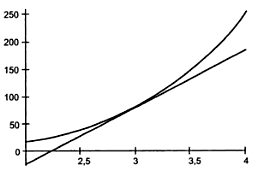
\includegraphics[page=1,scale=0.745]{img/jensen.png}
\end{figure} 

Utilizamos la linealidad y tenemos que:
\[
\mathbb{E}(g(X)) \geq \mathbb{E}(f(X)) = \mathbb{E}(aX+b)=a\mathbb{E}(X)+b=f(\mathbb{E}(X))=g(\mathbb{E}(X))
\]

\end{problem}

%%%%%%%%%%%%%%%%%%%%%%%%%%%%%%%%%%%%%%%%%%%%%%%%%%%%%%%%%%

%%%%%%%%%%%%%%%%%%  PROBLEMA 3.8  %%%%%%%%%%%%%%%%%%%%%%%%%
\begin{problem}[8] Probar que si $0 < r\le s \le \infty$,
 entonces $\|f\|_{L^r(\Omega, \mathcal{A}, P)}\le \|f\|_{L^s(\Omega, \mathcal{A}, P)}$, luego $L^s(\Omega, \mathcal{A}, P) \subset L^r(\Omega, \mathcal{A}, P)$ (sugerencia, usar Jensen o H\"older). Demostrar que si el espacio tiene medida infinita, esta
inclusi\'on puede fallar.
\solution

\begin{expla}
Tenemos que ver que para $0 <r\leq s \leq \infty$ se cumple que $\norm{f}_r \leq \norm{f}_s$, es decir:

\[
\left( \int \abs{f}^r dP \right)^{\frac{1}{r}} \leq \left( \int \abs{f}^s dP \right)^{\frac{1}{s}}
\]

%Por Hölder tenemos que: $\|fg\|_1 \leq \|f\|_p\|g\|_q$, que en nuestro caso sería: $\|f^2\|_1 \leq \|f\|_p\|f\|_q$


\end{expla}
Dos formas:
\begin{enumerate}
\item Usamos Jensen:

Jensen dice que para X variable aleatoria y $\phi$ función convexa pertenecientes a $L^1$, se tiene que:
\[
\phi(\mathbb{E}(X)) \leq \mathbb{E}(\phi(X))
\]


Tenemos que:

\[
\norm{f}_{L^r(\Omega, \algb{M}, P)} = \norm{f}_r= \left( \int_{\Omega} \abs{f}^r dP \right)^{\frac{1}{r}}
\]

Para simplificar la notación, omitiremos a partir de ahora $\Omega$ y dP. Usamos como función convexa $g(t)=\abs{t}^{\frac{s}{r}}$.

Por tanto tenemos que:
\[
g(\mathbb{E}(\abs{f}^r)) = \left(\int \abs{f}^r\right)^{\frac{s}{r}} \leq\int \left( \abs{f}^r \right)^{\frac{s}{r}} = \mathbb{E}(g(\abs{f}^r)) 
\]

Elevamos a $\frac{1}{s}$ a izquierda y derecha y obtenemos (desarrollamos desde el centro azul, hacia la izquierda y hacia la derecha):
\[
\norm{f}_r = \left(\int \abs{f}^r\right)^{\frac{1}{r}} = \textcolor{blue}{\left(\int \abs{f}^r\right)^{\frac{s}{rs}} \leq \left(\int \abs{f}^{\frac{rs}{r}}\right)^{\frac{1}{s}}} = \left(\int \abs{f}^s\right)^{\frac{1}{s}} = \norm{f}_s
\]



\item Usando Hölder:
si $f\in L^p$ y $g\in L^q$, entonces $fg\in L^1$, y $\|fg\|_1 \le \|f\|_p\|g\|_q$

Definimos la función $g=1$, que pertenece a $L^q$. Y cogemos $0<r<s<\infty$. Suponemos que $f \in L^s$ y $f\geq 0$, entonces tenemos que:
\[
\abs{f}=\abs{f}\cdot 1  \Leftrightarrow f^r = f^r \cdot 1
\]

Entonces queremos acotar $\int f^r \cdot 1$. Vemos que $f^r \in L^{\frac{s}{r}}$ y que $1 \in L^{\frac{s}{r}'}$  siendo $\frac{s}{r}'$ el conjugado de $\frac{s}{r}$, es decir cumple que ($\frac{1}{r/s}+\frac{1}{s/r} = 1$). Vamos a demostrar que  $f^r \in L^{\frac{s}{r}}$:
\[
 \int \abs{f^r}^{\frac{s}{r}} =  \int \abs f^s < \infty \text{ porque } f\in L^s
\]

Y ahora sí usamos Hölder:

\[
\int f^r = \int f^r \cdot 1 = \norm{f^r \cdot 1}_1 \leq \norm{f^r}_{\frac{s}{r}}\norm{1}_{\frac{s}{r}'}=\left( \int(f^r)^{\frac{s}{r}} \right)^{\frac{r}{s}} \cdot 1 = \left( \int f^s \right)^{\frac{r}{s}}
\]

Elevamos a izquierda y derecha por $\frac{1}{r}$ y obtenemos que:
\[
\left( \int f^r \right)^{\frac{1}{r}} \leq \left( \int f^s \right)^{\frac{1}{s}}
\]

Que es lo que queríamos demostrar.
\end{enumerate}



\end{problem}

%%%%%%%%%%%%%%%%%%%%%%%%%%%%%%%%%%%%%%%%%%%%%%%%%%%%%%%%%%



\newpage
\section{Hoja 4}

\textcolor{blue}{CORREGIDA Y CONTRASTADA CON LAS SOLUCIONES DEL PROFESOR SALVO SI SE INDICA LO CONTRARIO}

Salvo afirmaci\'on expresa en sentido
contrario se asume siempre que estamos trabajando en un espacio de probabilidad $(\Omega, \mathcal{A}, P)$,
que  $\mathcal{B}\subset \mathcal{A}$ es una sub-$\sigma$-\'algebra, que las funciones son medibles, etc..

Recordatorio: si $0 < p < \infty$, $\|f\|_p := \left(\int|f|^p\right)^{1/p}$, mientras que
$\|f\|_\infty$ denota el supremo esencial de $|f|$. 

%%%%%%%%%%%%%%%%%%  PROBLEMA 4.1  %%%%%%%%%%%%%%%%%%%%%%%%%
\begin{problem}[1] Ejemplos sobre la f\'ormula del cambio de variables.

\vskip .3 cm

a) Sea $X: [0,1)\to \mathbb{R}$ la variable aleatoria $X(w) := 2 w (\operatorname{mod}(1)$. Es decir,
si $w\in [0, 1/2)$, entonces  $X(w) = 2 w$, mientras que si  $w\in [1/2, 1)$, entonces  $X(w) = 2 w - 1$.
En  $[0,1)$ tenemos la probabilidad uniforme con los conjuntos de Borel (o Lebesgue, para este problema
da igual). Hallar la funci\'on de distribuci\'on $F_X$,  y  $P_X$, la probabilidad imagen o ley de $X$.
 Decidir razonadamente si $X$ es una v.a. continua, y en caso de respuesta afirmativa, hallar su funci\'on
de densidad $f_X$.

\vskip .3 cm

b) Sea $Y: [0,1]^2\to \mathbb{R}$ la variable aleatoria $Y(x,y) := y$.
En  $[0,1]^2$ tenemos la probabilidad uniforme con los conjuntos de Borel (o Lebesgue, para este problema
da igual). Hallar la funci\'on de distribuci\'on $F_Y$,  y  $P_Y$, la probabilidad imagen o ley de $Y$.
 Decidir razonadamente si $Y$ es una v.a. continua, y en caso de respuesta afirmativa, hallar su funci\'on
de densidad $f_Y$.

\vskip .3 cm


c) Decidir razonadamente si para toda funci\'on de Borel acotada $g:\mathbb{R}\to \mathbb{R}$,
$$\int_{ [0,1)} g(X(w)) dw = \int_{ [0,1]^2} g(Y(x,y)) dx dy.$$

\solution

\begin{expla}

\end{expla}

\spart 
Vemos que la variable aleatoria X(w) es una función que crece con pendiente 2 en el intervalo $[0,1/2)$ y en $[1/2,1)$:

\begin{figure}[h]
\centering
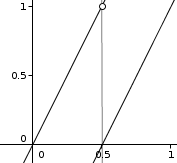
\includegraphics[page=1,scale=0.745]{img/f.png}
\end{figure} 

Por tanto, se ve que tiene la misma probabilidad de valer cualquier valor entre 0 y 1, la función de distribución será simplemente:

$$
F_x(x) =
  \left\lbrace
  \begin{array}{l}
     0 \text{ si } x < 0\\
     x \text{ si } x \in [0,1) \\
     1 \text{ si } x \geq 1 \\
  \end{array}
  \right.
$$

Por su parte, la ley de x, o $P_x$, recordemos que es:
$P_x(B) = P(X^{-1}(B)) = P(\{w \in \Omega : X(w) \in B\})=P(X \in B)$. En este caso coincide con la medida de Lebesgue de B.

Por ejemplo, si B es el intervalo $(1/2, 3/4)$, vemos que $X(w)$ toma esos valores en un exactamente $3/4-1/2=1/4$ de los valores de w.

Por tanto: $P_x(B)=\mu(B)$ (siendo $\mu$ la medida de Lebesgue).

Ahora queremos ver que X es una variable aleatoria continua. Nos remitimos a la definición de variable aleatoria continua:

X es una variable aleatoria continua $\Leftrightarrow$ $P_x$ es absolutamente continua con respecto a la medida de Lebesgue.

Recordemos lo que significa que una medida $\mu$ sea absolutamente continua con respecto a otra $\nu$:  $\mu << \nu$ si $\mu(A)=0 \Rightarrow \nu(A)=0$

Tenemos que ver que $P_x$ es absolutamente continua con respecto a la medida de Lebesgue, lo que es obvio ya que $P_x(B)=\mu(B)$. La llamaremos $P_{x1}$ para diferenciarla del apartado B.

Por último definimos la función de densidad $f_x(x)$.

$$
f_x(x) =
  \left\lbrace
  \begin{array}{l}
     0 \text{ si } x < 0\\
     1 \text{ si } x \in [0,1) \\
     0 \text{ si } x \geq 1 \\
  \end{array}
  \right.
$$
\spart
Obtenemos el mismo resultado que en el caso anterior para $F_x$ y para $f(x)$.

También para $P_x$, que lo llamaremos $P_{x2}(B)=\mu(B)$.


\spart 

Tenemos que demostrar que:

$$\int_{ [0,1)} g(X(w)) dw = \int_{ [0,1]^2} g(Y(x,y)) dx dy.$$

Vamos a utilizar la fórmula del cambio de variable:
\[
\int_{\Omega}g(X(w))dP(w)=\int_{\mathbb{R}}g(x)dP_X(x)
\]

Para aplicar la fórmula del cambio de variable, lo único que tenemos que hacer es cambiar los límites de integración por los valores en los que se mueven $X(w)$ e $Y(x,y)$, y cambiar la medida sobre la que se integra.

Empezamos por el primer término, y le aplicamos la fórmula del cambio de variable:
$$\int_{ [0,1)} g(X(w)) dw = \int_{ [0,1)} g(2w \mod{1}) dw= \int_{ [0,1)} g(x) dP_{x1}(x)$$

Ahora cogemos el segundo término:
$$\int_{ [0,1]^2} g(Y(x,y)) dx dy = \int_{ [0,1)} g(y) dP_{x2}(y)$$

Que son iguales ya que $P_{x2}(x) = P_{x1}(x)$.

\textcolor{blue}{Solucion del profesor al apartado c:}
\[
\int_0^1 g(X(w)) dw \stackrel{FCV}{=} \int_{\mathbb{R}}g(x)dP_x(x)= \int_{-\infty}^{\infty}g(x)dx
\]

\[
\int_0^1 \int_0^1 g(Y(x,y))dxdy \stackrel{FCV}{=} \int_{\mathbb{R}}g(y)dP_y(y)= \int_{-\infty}^{\infty}g(y)dy
\]

\end{problem}
%%%%%%%%%%%%%%%%%%%%%%%%%%%%%%%%%%%%%%%%%%%%%%%%%%%%%%%%%%


%%%%%%%%%%%%%%%%%%  PROBLEMA 4.2  %%%%%%%%%%%%%%%%%%%%%%%%%
\begin{problem}[2] Demostrar la desigualdad de Jensen condicional: si $X:\Omega\to I\subset \mathbb{R}$, donde
$I$ es un intervalo en $\mathbb{R}$, $g:I\to \mathbb{R}$ es convexa, y $X, g(X) \in L^1$, entonces
 $g(E(X|\mathcal{B})) \le E(g(X)|\mathcal{B})$. 

\solution

\begin{expla}
Razonamiento parecido que en el ejercicio 7 de la hoja 3.
\end{expla}
Dada una función convexa $\phi$. Vemos que la función $\phi=\sup_{L} {L \leq \phi}$. Siendo L rectas que quedan por debajo de $\phi$ o que coinciden tangencialmente a ella.

Además: $L(t)=a+bt$. Lo simplificamos por continuidad para valores $a,b \in \mathbb{Q}^2$.

Por tanto tenemos de momento que $L \leq \phi$, y por tanto que $L(X) \leq \phi(X)$. De esto obtenemos lo siguiente:
\[
\mathbb{E}(\phi(X)|\algb{B}) \stackrel{positividad}{\geq} \mathbb{E}(L(X)|\algb{B}) = \mathbb{E}(a+bX|\algb{B}) = a+b\mathbb{E}(X|\algb{B}) = L(\mathbb{E}(X|\algb{B}))
\]

Y para terminar:
\[
\mathbb{E}(\phi(X)|\algb{B}) \geq \sup L(\mathbb{E}(X|\algb{B}))=\phi(\mathbb{E}(X|\algb{B}))
\]


\end{problem}

%%%%%%%%%%%%%%%%%%%%%%%%%%%%%%%%%%%%%%%%%%%%%%%%%%%%%%%%%%

%%%%%%%%%%%%%%%%%%  PROBLEMA 4.3  %%%%%%%%%%%%%%%%%%%%%%%%%
\begin{problem}[3] Sean $p,q \ge 1$ exponentes conjugados, es decir, $p$ y $q$ satisfacen
$1/p + 1/q =1$ (si $p=1$, entonces $q = \infty$, y viceversa).
Dado un espacio de probabilidad  $(\Omega, \mathcal{A}, P)$, enunciar y probar la desigualdad condicional de 
H\"older. Sugerencia: usar la desigualdad de H\"older.
\solution
\textcolor{red}{ESTE EJERCICIO ESTA MAAAAAL, COMO EL CULO VAYA, Y NO TENEMOS LA SOLUCION, DIJO QUE LO MIRARAMOS EN INTERNET}

\begin{expla}
Tenemos que demostrar que:
\[
\mathbb{E}(\abs{XY}|\algb{B}) \leq \mathbb{E}(\abs{X}^p|\algb{B})^{\frac{1}{p}} \mathbb{E}(\abs{Y}^q|\algb{B})^{\frac{1}{q}}
\]

Por ser esperanzas condicionadas, tenemos que cumplen que son $\algb{B}$-medibles y que:
$\forall B \in \algb{B}$, $\int_{B}\mathbb{E}(X|\algb{B})dP=\int_{B}XdP$. Además estas dos propiedad definen la esperanza condicionada de modo único.

\end{expla}
Empezamos aplicando dicha propiedad sobre $\mathbb{E}(\abs{XY}|\algb{B})$:
\[
\int_{\Omega}\mathbb{E}(\abs{XY}|\algb{B}) = \int_{\Omega}\abs{XY} = \norm{XY} \leq \norm{X}_p \norm{Y}_q = \left( \int_{\Omega} \abs{X}^p \right)^{\frac{1}{p}} \left( \int_{\Omega} \abs{X}^q \right)^{\frac{1}{q}} =  
\]

\[
= \left( \int_{\Omega} \mathbb{E}(\abs{X}^p|\algb{B}) \right)^{\frac{1}{p}} \left( \int_{\Omega} \mathbb{E}(\abs{X}^q|\algb{B}) \right)^{\frac{1}{q}}
\]

Por tanto, como esta propiedad define la esperanza de modo único, vemos que:

\[
\mathbb{E}(\abs{XY}|\algb{B}) \leq \mathbb{E}(\abs{X}^p|\algb{B})^{\frac{1}{p}} \mathbb{E}(\abs{Y}^q|\algb{B})^{\frac{1}{q}}
\]

\end{problem}

%%%%%%%%%%%%%%%%%%%%%%%%%%%%%%%%%%%%%%%%%%%%%%%%%%%%%%%%%%

%%%%%%%%%%%%%%%%%%  PROBLEMA 4.4  %%%%%%%%%%%%%%%%%%%%%%%%%
\begin{problem}[4] Probar que si $X := \{X_n\}_{n=0}^{\infty}$  es una martingala adaptada a la filtraci\'on
$\{\mathcal{A}_n\}_{n=0}^{\infty}$, entonces para todo $n>0$ tenemos 
$EX_n = EX_0$. 
Enunciar los resultados an\'alogos para sub y supermartingalas.
\solution

\begin{expla}
Nos basamos en dos propiedades:
\begin{enumerate}
\item Por parte de la martingala usamos que:
$$\forall_n, \mathbb{E}(X_{n+1}|\algb{M}_n)=X_n$$
\item Por parte de la probabilidad condicionada usamos que:
$$\forall B \in \algb{B}, \int_{B}\mathbb{E}(X|\algb{B})dP=\int_{B}XdP$$
\end{enumerate}
\end{expla}
Aplicamos 1) sobre $X_n$ en el primer paso, 2) en el tercero (combinado con que $\Omega$ pertenece a $\algb{A}_n$), y definición de esperanza en el segundo y en el cuarto.
\[
\mathbb{E}(X_n) =\mathbb{E}(\mathbb{E}(X_{n+1}|\algb{A}_n)) = \int_{\Omega} \mathbb{E}(X_{n+1}|\algb{A}_n) dP = \int_{\Omega} X_{n+1}dP = \mathbb{E}(X_{n+1})
\]

Siguiendo este procedimiento n veces de derecha a izquierda llegamos a lo que nos piden: $\mathbb{E}(X_n) = \mathbb{E}(X_0)$.

Para las submartingalas y supermartingalas es lo mismo solo que poniendo $\geq$ y $\leq$ respectivamente.

\end{problem}

%%%%%%%%%%%%%%%%%%%%%%%%%%%%%%%%%%%%%%%%%%%%%%%%%%%%%%%%%%

%%%%%%%%%%%%%%%%%%  PROBLEMA 4.5  %%%%%%%%%%%%%%%%%%%%%%%%%
\begin{problem}[5] Probar que si $X := \{X_n\}_{n=0}^{\infty}$  es una martingala adaptada a la filtraci\'on
$\{\mathcal{A}_n\}_{n=0}^{\infty}$, entonces para todo $m, n\ge 0$ tenemos
$E(X_{n + m}|\mathcal{A}_n) = X_n$. Enunciar los resultados an\'alogos para sub y supermartingalas.
\solution

\begin{expla}
Nos basamos en dos propiedades:
\begin{enumerate}
\item Por parte de la martingala usamos que:
$$\forall_n, \mathbb{E}(X_{n+1}|\algb{M}_n)=X_n$$
\item Propiedad de la torre (la 7) de la probabilidad condicionada:
Sean $\algb{C} \subset \algb{B} \subset \algb{M}$ $\salgb$s, si $X \in L^ 1(\algb{M})$ entonces:
\begin{itemize}
\item $\mathbb{E}(\mathbb{E}(X|\algb{C})|\algb{B}) = \mathbb{E}(X|\algb{C})$.
\item $\mathbb{E}(\mathbb{E}(X|\algb{B})|\algb{C}) = \mathbb{E}(X|\algb{C})$.
\end{itemize}
\end{enumerate}
\end{expla}
En el caso de las martingalas tenemos que:
$\algb{A}_n \subset \algb{A}_{n+1} \subset \algb{A}_{n+2}...$

\[
X_n = \mathbb{E}(X_{n+1}|\algb{A}_n) = \mathbb{E}(\mathbb{E}(X_{n+2}|\algb{A}_{n+1})|\algb{A}_n) = \mathbb{E}(X_{n+2}|\algb{A}_n) =
\]

\[
= \mathbb{E}(\mathbb{E}(X_{n+3}|\algb{A}_{n+2})|\algb{A}_n) =
\mathbb{E}(X_{n+3}|\algb{A}_n) = ... = \mathbb{E}(X_{n+m}|\algb{A}_n)
\]

Para las submartingalas y supermartingalas es lo mismo solo que poniendo $\geq$ y $\leq$ respectivamente.
\end{problem}

%%%%%%%%%%%%%%%%%%%%%%%%%%%%%%%%%%%%%%%%%%%%%%%%%%%%%%%%%%

%%%%%%%%%%%%%%%%%%  PROBLEMA 4.6  %%%%%%%%%%%%%%%%%%%%%%%%%
\begin{problem}[6] C\'omo ganar un euro con probabilidad 1, en un juego justo: la estrat\'egia del doble o nada.
Apostamos un euro a que sale cara. Si sale cara nos plantamos, si sale cruz apostamos
2 euros a que sale cara. Si sale cara nos plantamos, si sale cruz apostamos
4 euros a que sale cara. Etc.. Demostrar que la  estrat\'egia anterior gana un euro
 con probabilidad 1.
\solution

\begin{expla}

\end{expla}
Llamamos $X_n=$ ganancias acumuladas después de n partidas. Los eventos w será una sucesión de n dígitos que serán 1 si sale cara y -1 si sale cruz.

Vemos que existe T tal que $\mathbb{E}(X_0) = 0 < 1 = \mathbb{E}(X_t)$. Esto quiere decir que no se cumple ninguna de las 3 condiciones del teorema de parada opcional de Doob.

Por ejemplo dado $w_0=(1,-1,1,...)$ entonces $T(w_0)=1$. Dado $w_1=(-1,-1,1,...)$ entonces $T(w_1)=3$. Dado $w_2=(-1,-1,-1,1,...)$ entonces $T(w_0)=4$. 

Además vemos que P(no salga cara)=$\lim_{n \rightarrow \infty} \frac{1}{2^n} = 0$. Y $P(T=n)=\frac{1}{2^n}$.

Vamos a ver una a una las condiciones de parada opcional de Doob:
\begin{enumerate}
\item $\exists M >0$ tal que $T \leq M$. 

Esta condición falla ya que $T \notin L^{\infty}$ (no está acotada, no tiene máximo su gráfica vaya)
\item $\forall n \geq 0$ y casi todo $w \in \Omega$, $\abs{X_n(w)} \leq M$ con $M >0$ fijo.

También falla ya que se puede cumplir que para cierto w:$\abs{X_n(w)}=\abs{1-2^n} \stackrel{n \rightarrow \infty}{\rightarrow} \infty$.

Por tanto este valor no esta acotado por ningún M fijo.

\item $\mathbb{E}(T)<\infty$ y $\exists M > 0$ tal que para casi todo w y todo n $\abs{X_{n+1}(w) - X_n(w)} \leq M$.

$\mathbb{E}(T)=\sum_{n=1}^{\infty} n \cdot P(T=n) = \sum_{n=1}^{\infty} n \cdot \frac{1}{2^n} < \infty$,de hecho es 2, ya que:

\[
\sum_{n=0}^{\infty} t^n = \frac{1}{1-t} \text{ para } \abs{t}<1
\]

Y tenemos que:
\[
\frac{d}{dt}(\frac{1}{1-t})=\frac{1}{(1-t)^2}
\]

Por tanto:
\[
\sum_{n=0}^{\infty} nt^{n-1} = \frac{1}{(1-t)^2} \text{ para } \abs{t}<1
\]

Y concluimos que con $t=\frac{1}{2}$:
\[
t \sum_{n=1}^{\infty}nt^{n-1}=\frac{t}{(1-t)^2} \rightarrow \sum_{n=1}^{\infty}nt^{n-1} = \frac{\frac{1}{2}}{(1-\frac{1}{2})^2}=2
\]

Pero $\abs{X_{n+1}(w)-X_n(w)} = 2^{n-1}  \stackrel{n \rightarrow \infty}{\rightarrow} \infty$

Por tanto tampoco existe un M fijo y tampoco se cumple la propiedad.
\end{enumerate}

Concluimos que no se cumple ninguna de las 3 propiedades, por tanto, sí ganamos un euro con probabilidad 1.
\end{problem}

%%%%%%%%%%%%%%%%%%%%%%%%%%%%%%%%%%%%%%%%%%%%%%%%%%%%%%%%%%

\newpage
\section{Hoja 5}

\textcolor{blue}{CORREGIDA Y CONTRASTADA CON LAS SOLUCIONES DEL PROFESOR SALVO SI SE INDICA LO CONTRARIO}

Salvo afirmaci\'on expresa en sentido
contrario se asume siempre que estamos trabajando en un espacio de probabilidad $(\Omega, \mathcal{A}, P)$,
que  $\mathcal{B}\subset \mathcal{A}$ es una sub-$\sigma$-\'algebra, que las funciones son medibles, etc.


Recordatorio: si $1\le p < \infty$, $\|f\|_p := \left(\int|f|^p\right)^{1/p}$, mientras que
$\|f\|_\infty$ denota el supremo esencial de $|f|$. De hecho, la definici\'on
 $\|f\|_p := \left(\int|f|^p\right)^{1/p}$ tiene sentido para cualquier $p > 0$ finito, pero puede
demostrarse que si $p < 1$ esta expresi\'on no define una norma.

%%%%%%%%%%%%%%%%%%  PROBLEMA 5.1  %%%%%%%%%%%%%%%%%%%%%%%%%
\begin{problem}[1] Sea $X: [0,1) \to [0,1)$ la identidad $X(w) = w$, donde a $[0,1)$ se le asigna la
probabilidad uniforme (en este caso, la medida de Lebesgue). Sea  $\mathcal{A}_n := \sigma([0,1/2^n), [1/2^n,2/2^n) , \dots,
[ (2^n - 1)/2^n, 1))$ la $ \sigma$-\'algebra generada por los intervalos di\'adicos $ [j/2^n,(j + 1)/2^n)$, $j = 1\dots, n-1$.
Calcular $E(X|\mathcal{A}_n)$. Decidir razonadamente si la sucesi\'on de v.a. $ \{E(X|\mathcal{A}_n)\}_{n=0}^{\infty}$
converge (y en caso de respuesta afirmativa, determinar a qu\'e) en alguno de los siguientes sentidos:
a) uniformemtente, b) en $L^p$, determinando para que valores de $p$ hay convergencia, c) en casi todo punto,
d) en medida.
\solution

\begin{expla}
Vemos que $\algb{M}_n$ esta generada a partir de una partición, de elementos disjuntos, y por tanto:
\[
\mathbb{E}(X|\algb{M}_n)(w)=\frac{1}{P(A_i)} \int_{A_i}X(w)dP(w)
\]

Definimos $\mathbb{E}(X|\algb{M}_1)(w)$

$$
\mathbb{E}(X|\algb{M}_1)(w) =
  \left\lbrace
  \begin{array}{l}
      \frac{1}{P([0, 1/2))}\int_{[0,1/2)}wdP(w)= \left.2 \frac{w^2}{2}\right|_0^{1/2} = 1/4  \\
     ... 3/4  \\
  \end{array}
  \right.
$$

Y $\mathbb{E}(X|\algb{M}_2)(w)$:
$$
\mathbb{E}(X|\algb{M}_2)(w) =
  \left\lbrace
  \begin{array}{l}
      \frac{1}{8}\\
      \frac{3}{8}\\
      \frac{5}{8}\\
      \frac{7}{8}\\
  \end{array}
  \right.
$$

\end{expla}

Obtenemos que:
$$
\mathbb{E}(X|\algb{M}_n)(w) =
  \left\lbrace
  \begin{array}{l}
      \frac{1}{2^{n+1}}\\
      \frac{3}{2^{n+1}}\\
      ...\\
      \frac{2^{n+1}-1}{2^{n+1}}\\
  \end{array}
  \right.
$$

Por tanto, observamos, que  $\mathbb{E}(X|\algb{M}_n)(w)$ converge a X(w)=w.

\begin{enumerate}
\item Convergencia uniforme:  una sucesión $f_n:I\rightarrow \mathbb{R}$ converge uniformemente a $f:I\rightarrow \mathbb{R}$ si: $\forall \epsilon >0$,  $\exists N_{\epsilon}$ tal que $\forall n \geq N_{\epsilon}$ se cumple que $\abs{f_n(x)-f(x)}<\epsilon$ $\forall x \in I$. Es decir si:
\[
\lim_{n \rightarrow \infty} \norm{f_n - f}_{\infty} = 0
\]

O equivalentemente si:
\[
\lim_{n \rightarrow \infty} \sup_{x \in I}\{\abs{f_n(x)-f(x)} \}=0
\]

En este caso sabemos que converge uniformemente ya que $\frac{1}{2^{n+1}}$ es una cota independiente de w.

La convergencia uniforme implica todas las demás. Aún así, vamos a repasarlas.

\item Convergencia en $L^p$:
\[
f_n \stackrel{L_p (n\rightarrow \infty)}{\rightarrow} g \Leftrightarrow \norm{f_n -g}_p  \rightarrow 0 \Leftrightarrow \int{\abs{f_n -g}^pd\mu} \rightarrow 0
\]

Por tanto, tenemos que ver que:
\[
\int \abs{\mathbb{E}(X|\algb{M}_n)(w)-X(w)| }^p \rightarrow 0
\]

Pero sabiendo que converge uniformemente no nos complicamos la vida y lo usamos, para $0<r<\infty$ tenemos que:
\[
0 \leq \lim_{n \rightarrow \infty} \norm{X-X_n}_{r} \leq \lim_{n \rightarrow \infty} \norm{X-X_n}_{\infty} = 0 \text{ por converger uniformemente}
\]


\item Convergencia en casi todo punto o puntual: una sucesión $f_n:I\rightarrow \mathbb{R}$ converge puntualmente a $f:I\rightarrow \mathbb{R}$ si: $\forall \epsilon >0$ y $\forall x \in I$, $\exists N_{\epsilon, x}$ tal que $\forall n \geq N_{\epsilon, x}$ se cumple que $\abs{f_n(x)-f(x)}<\epsilon$. Es decir si:
\[
\lim_{n \rightarrow \infty} f_n(x)-f(x)=0
\]

En este caso sabemos que converge puntualmente. Nos sirve la misma cota que hemos usado para la convergencia uniforme. Además, convergencia uniforme implica convergencia puntual como ya hemos dicho.

\item Convergencia en medida o en probabilidad:
Si $\forall \epsilon >0$, $\lim_{n \rightarrow \infty}P(\abs{X-X_n}\geq \epsilon)=0$.

Por ser convergente uniformemente, converge en medida.



%Pero por definición de esperanza condicionada y por ser X $\algb{M}_n$-medible, tenemos que:
%\[
%\mathbb{E}(X|\algb{M}_n) = X
%\]

%Elevamos a p e integramos y ya tenemos la igualdad que buscamos
\end{enumerate}

\end{problem}
%%%%%%%%%%%%%%%%%%%%%%%%%%%%%%%%%%%%%%%%%%%%%%%%%%%%%%%%%%


%%%%%%%%%%%%%%%%%%  PROBLEMA 5.2  %%%%%%%%%%%%%%%%%%%%%%%%%
\begin{problem}[2]  Probar que si $X := \{X_n\}_{n=0}^{\infty}$  es una submartingala, y
$0  <  r\le s\le \infty$, entonces $\|X\|_r  \le \|X\|_s$, donde 
$\|X\|_p := \sup_{n\in \mathbb{N}} \|X_n\|_{p}$. 
\solution

\begin{expla}
utilizamos el ejercicio 3.8, es decir, que si $0<r\leq s \leq \infty$, entonces $\norm{f}_r \leq \norm{f}_s$.

La norma de una martingala se define:
\[
\norm{X}_p = \sup_n \norm{X_n}_p
\]
\end{expla}

Tenemos que ver que:
\[
\sup_n \norm{X_n}_r \leq \sup_n \norm{X_n}_s
\]

Entonces, existirá un p tal que:

\[
\sup_n \norm{X_n}_r  = \norm{X_p}_r \leq \norm{X_p}_s \leq \sup_n \norm{X_n}_s
\]

\end{problem}

%%%%%%%%%%%%%%%%%%%%%%%%%%%%%%%%%%%%%%%%%%%%%%%%%%%%%%%%%%

%%%%%%%%%%%%%%%%%%  PROBLEMA 5.3  %%%%%%%%%%%%%%%%%%%%%%%%%
\begin{problem}[3] Probar que si $X := \{X_n\}_{n=0}^{\infty}$  es una martingala, y $ \|X\|_s <\infty$, donde 
$1\le s < \infty$, entonces  $Y := \{|X_n|^s\}_{n=0}^{\infty}$  es una submartingala
en $L^1$. 
\solution

\begin{expla}
Sabemos que:
\begin{enumerate}
\item $X_n = \mathbb{E}(X_{n+1}|\algb{A}_n)$
\item $\norm{X_n}_s = (\int \abs{X_n}^s)^{\frac{1}{s}} < \infty$
\end{enumerate} 
\end{expla}
Comprobamos las 3 condiciones que debe cumplir una martingala
\begin{enumerate}
\item Hay que ver que $\sup \norm{\abs{X_n}^s} < \infty$:
\[
\sup \int_{\Omega} \abs{X_n}^s dP =  \sup \norm{X_n}_s^s < \infty \text{ por 2.}
\]
\item La composición de funciones medibles es medible. \textcolor{red}{¿Qué estamos componiendo?}
\item Tenemos que probar que: $\mathbb{E}(\abs{X_{n+1}}^s|\algb{A}_n) \geq \abs{X_n}^s$:
\[
\mathbb{E}(X_{n+1}|\algb{A}_n) = X_n \Leftrightarrow \abs{X_n}^s  = \abs{\mathbb{E}(X_{n+1}|\algb{A}_n)}^s \stackrel{JensenCondicional}{\leq} \mathbb{E}(\abs{X_{n+1}}^s|\algb{A}_n)
\]
\end{enumerate}


\end{problem}

%%%%%%%%%%%%%%%%%%%%%%%%%%%%%%%%%%%%%%%%%%%%%%%%%%%%%%%%%%

%%%%%%%%%%%%%%%%%%  PROBLEMA 5.4  %%%%%%%%%%%%%%%%%%%%%%%%%
\begin{problem}[4]  Sea $\{X_n\}_{n=0}^{\infty}$ una sucesi\'on de v.a.i.i.d., tales que 
$P(X_i = 1)= P(X_i = -1) = 1/2$, y sea $S_n := \sum_{i=0}^n X_i$.
Vimos en clase que $S := \{S_n\}_{n=0}^{\infty}$  es una martingala adaptada a la filtraci\'on
$\{\mathcal{A}_n\}_{n=0}^{\infty}$, donde $\mathcal{A}_n := \sigma(X_0, \dots, X_n)$.
Sea $c > 0$. 
Calcular $\lim_{n\to \infty} P( -c < S_n < c)$. Sugerencia: se puede usar el Teorema del L\'{\i}mite Central,
visto en Probabilidad I.
 Decidir razonadamente si la martingala $S = \{S_n\}_{n=0}^{\infty}$ 
 est\'a en $L^1$, es decir, si $\sup_n \|S_n\|_1 < \infty$. Decidir razonadamente
si $S_n$ converge en casi todo punto a una funci\'on $S_ \infty$ tal que
$P(|S_\infty| = \infty) = 0$. 

\solution
\textcolor{red}{ESTE EJERCICIO ESTA MAL, A LA ESPERA DE UNA RESPUESTA}

\begin{expla}
El teorema central del límite dice que:
\[
\lim_{n \rightarrow \infty} P(\sqrt{n}(S_n - \mu) \leq \sigma t) = N(0,1)(t)
\]

Que para valores grandes de n, es equivalente a decir:
\[
\lim_{n \rightarrow \infty} P(\sqrt{n}(S_n - \mu) \leq t) = N(0,1)(\frac{t}{\sigma})
\]

Sabemos que $\bar{X} = \frac{1}{n} \sum_{i=1}^{n}X_i$

\end{expla}

En nuestro caso tenemos que:

\[
\bar{S_n} = \frac{1}{n} \sum_{i=1}^{n}S_n
\]

\[
\mu = \mathbb{E}(S_n)= 0
\]

\[
\sigma^2 = V(S_n) = \mathbb{E}(S_n^2)-\mathbb{E}(S_n)^2 = 1 - 0 = \frac{1}{n} 
\]

\[
\sigma = \frac{1}{\sqrt{n}}
\]


Vamos a normalizar la probabilidad, y dejarlo de la forma:
\[
P(\frac{\sqrt{n}(\bar{S_n}-\mu)}{\sigma} \leq z)
\]

En nuestro caso, nos debería quedar:
\[
P(n\bar{S_n}\leq z)
\]


Así, usamos que $S_n = n\bar{S_n}$, y nos queda que:
\[
P(-c<S_n<c)=P(-c<n\bar{S_n}<c)=P(n\bar{S_n}>-c)-P(n\bar{S_n}>c)=
\]

\[
=1-2P(n\bar{S_n}>c) \rightarrow 1-N(0,1)(c)
\]



\end{problem}

%%%%%%%%%%%%%%%%%%%%%%%%%%%%%%%%%%%%%%%%%%%%%%%%%%%%%%%%%%


\newpage
\section{Hoja 6}

\textcolor{blue}{CORREGIDA Y CONTRASTADA CON LAS SOLUCIONES DEL PROFESOR}

Salvo afirmaci\'on expresa en sentido
contrario se asume siempre que estamos trabajando en un espacio de probabilidad $(\Omega, \mathcal{A}, P)$,
que  $\mathcal{B}\subset \mathcal{A}$ es una sub-$\sigma$-\'algebra, que las funciones son medibles, etc.

Recordatorio: si $1\le p < \infty$, $\|f\|_p := \left(\int|f|^p\right)^{1/p}$, mientras que
$\|f\|_\infty$ denota el supremo esencial de $|f|$. De hecho, la definici\'on
 $\|f\|_p := \left(\int|f|^p\right)^{1/p}$ tiene sentido para cualquier $p > 0$ finito, pero puede
demostrarse que si $p < 1$ esta expresi\'on no define una norma.


%%%%%%%%%%%%%%%%%%  PROBLEMA 6.1  %%%%%%%%%%%%%%%%%%%%%%%%%
\begin{problem}[1] Sea $\{\mathcal{A}_n\}_{n=0}^{\infty}$ una filtraci\'on de sub-$\sigma$-\'algebras de $\mathcal{A}$,
y sea $Y\in L^1(\Omega, \mathcal{A}, P)$. Demostrar que $X_n:=  E(Y|\mathcal{A}_n)$ define una
martingala en $L^1$. Decidir razonadamente si $X_n$ converge a $Y$ en $L^1$.

\solution

\begin{expla}
Vamos a ver que $X_n:=  E(Y|\mathcal{A}_n)$ cumple las tres propiedades de una martingala en $L^1$:
\begin{enumerate}
\item $\forall n$, $X_n \in L^1(\Omega, \algb{A}. P)$.
\item $\forall n$, $X_n$ es $\algb{A}_n$-medible.
\item $\forall_n$, $\mathbb{E}(X_{n+1}|\algb{A}_n)=X_n$ c.s.

\end{enumerate}

\end{expla}
Sabemos que X es una martingala en $L^p$ con $1\leq p \leq \infty$, si X es una martingala y $\norm{X}_p = \sup_{n}\norm{X_n}_p < \infty$. (Por una definición vista en la teoría en martingalas)

En este caso: $X_n = \mathbb{E}(Y|\algb{A}_n)$. Por la propiedad 4 de la esperanza condicionada, tenemos que esta es una contracción en $L^1$, es decir: $\norm{Y}_1 \geq \norm{\mathbb{E}(Y|\algb{A}_n)}_1$. Y nos queda:

\[
\sup_{n}\norm{X_n}_1 = \sup_{n}\norm{\mathbb{E}(Y|\algb{A}_n)}_1 \leq \norm{Y}_1 < \infty
\]

Por tanto, ya hemos demostrado la segunda parte de la definición.

Ahora vamos a ver que cumple las tres propiedades de una martingala:

\begin{enumerate}
\item Obvio por lo que acabamos de hacer. $X_n = \mathbb{E}(Y |\algb{A}_n) \in L^1$ ya que el supremo de esos $X_n$ pertenece a $L^1$.

Otra opción:
Tenemos que ver que $\mathbb{E}(Y|\mathcal{A}_n) \in L^1$, es decir, que $\int_{\Omega} \abs{\mathbb{E}(Y|\mathcal{A}_n)} dP < \infty$. 

Tenemos una propiedad de las esperanzas condicionadas (la tercera) que dice que: $\abs{\mathbb{E}(X|\algb{B})} \leq \mathbb{E}(\abs{X}|\algb{B})$.

En nuestro caso, aplicando esta propiedad y la segunda propiedad de la definición de esperanza condicionada ($\forall B \in \algb{B}$, $\int_{B}\mathbb{E}(X|\algb{B})dP=\int_{B}XdP$), nos queda que:

\[
\int_{\Omega} \abs{\mathbb{E}(Y|\mathcal{A}_n)} \leq  \int_{\Omega} \mathbb{E}(\abs{Y}|\mathcal{A}_n) = \int_{\Omega} \abs{Y} < \infty
\]


\item Tenemos que ver que $\mathbb{E}(Y|\mathcal{A}_n)$ es $\algb{A}_n$-medible. Lo cual es cierto por definición de esperanza condicionada.

\item Tenemos que ver que $\mathbb{E}(\mathbb{E}(Y|\mathcal{A}_{n+1})|\mathcal{A}_n) = \mathbb{E}(Y|\mathcal{A}_n)$

Aplicamos la regla de la torre (séptima propiedad de una esperanza condicionada), puesto que $\algb{A}_n \subset \algb{A}_{n+1}$, y sale directamente:

\[
\mathbb{E}(\mathbb{E}(Y|\mathcal{A}_{n+1})|\mathcal{A}_n) = \mathbb{E}(Y|\mathcal{A}_n)
\]

\end{enumerate}
Ahora vamos a ver razonadamente si $X_n$ converge a Y en $L^1$. Por definición de convergencia tenemos que ver que:
\[
X_n \stackrel{L_1 (n\rightarrow \infty)}{\rightarrow} Y \Leftrightarrow \norm{X_n -Y}_1  \rightarrow 0 \Leftrightarrow \int{\abs{X_n -Y}dP} \rightarrow 0 \Leftrightarrow \int{\abs{\mathbb{E}(Y|\mathcal{A}_n) -Y}dP} \rightarrow 0
\]


Buscamos un contraejemplo:
Sea $(\Omega, \algb{A}, P)=([0,1], Borel, \lambda)$ y $\algb{A}_n = \algb{A}_0 = \{\emptyset, [0,1] \}$. Entonces dada la variable aleatoria $Y(w)=w$, esta define una martingala en $L^1$. Sin embargo:


\[
\mathbb{E}(Y|\algb{A}_n)=\mathbb{E}(Y) = \frac{1}{2} \rightarrow \frac{1}{2}=X_{\infty}\neq Y
\]

Por tanto no converge.





\end{problem}
%%%%%%%%%%%%%%%%%%%%%%%%%%%%%%%%%%%%%%%%%%%%%%%%%%%%%%%%%%


%%%%%%%%%%%%%%%%%%  PROBLEMA 6.2  %%%%%%%%%%%%%%%%%%%%%%%%%
\begin{problem}[2] Sea $X := \{X_n\}_{n=0}^{\infty}$   una martingala en $L^2$. Probar que los incrementos 
son ortogonales, donde los incrementos se definen como $Y_0 := X_0$, y 
para $n > 0$, $Y_n := X_n - X_{n-1}$. Es decir, demostrar que si $j\ne k$, entonces
$(Y_j, Y_k) = \int Y_j Y_k = 0$. 
\solution

\begin{expla}

\obs Si $k>j$:
\begin{itemize}
\item $\mathbb{E}(X_k|\algb{A}_j) = X_j$

Viene del ejercicio 4.5: $\mathbb{E}(X_{n+m}|\algb{A}_n)=X_n$

\item Si $j,i < k$, entonces: $\mathbb{E}(X_j-X_i|\algb{A}_k)=X_j-X_i$  (por lo anterior)

\item $\mathbb{E}(X_j|\algb{A}_k) = X_j$

Como $\algb{A}_j \subset \algb{A}_k$, y $X_j$ es $\algb{A}_j$-medible, entonces también es $\algb{A}_k$-medible. Y ahora solo hay que aplicar la observación de la propiedad 6 de la esperanza condicionada (Si X es $\algb{B}$-medible, entonces $\mathbb{E}(X|\algb{B})=X$). 

\item Si $m,n > j$, entonces: $\mathbb{E}(X_m-X_n|\algb{A}_j)=X_j-X_j=0$  (por lo anterior)
\end{itemize}
\end{expla}



Si $k>j$ y $j=0$ (se explican los pasos debajo):
\[
\mathbb{E}\left[(X_k-X_{k-1})X_0\right] = \mathbb{E}\left( \mathbb{E}\left[(X_k-X_{k-1})X_0|\algb{A}_0\right]\right)= \mathbb{E}\left(X_0 \cdot \mathbb{E}\left[(X_k-X_{k-1})|\algb{A}_0\right]\right) =
\]
\[
= \mathbb{E}\left(X_0 \cdot (X_0-X_0)\right)  = 0
\]

El primer paso, es por definición de esperanza condicionada, sea $\mathbb{E}(X|\algb{B})$, se cumple que para todo $B \in \algb{B}$ y en particular para $\Omega$:
\[
\int_{\Omega}\mathbb{E}(X|\algb{B}) = \int_{\Omega}X \Leftrightarrow \mathbb{E}(\mathbb{E}(X|\algb{B})) = \mathbb{E}(X)
\]

El segundo paso es por la propiedad 6 de esperanza condicionada, ya que $X_0$ es $\algb{A}_0$-medible.

El tercer paso es por la linealidad y la primera y segunda observación que hemos escrito.


De manera general con $k>j$:
\[
\mathbb{E}\left[(X_k-X_{k-1})(X_j-X_{j-1})\right] = \mathbb{E}\left( \mathbb{E}\left[(X_k-X_{k-1})(X_j-X_{j-1})|\algb{A}_j\right]\right) =
\]
\[
= \mathbb{E}\left((X_j-X_{j-1}) \cdot \mathbb{E}\left[(X_k-X_{k-1})|\algb{A}_j\right]\right)= \mathbb{E}\left((X_j-X_{j-1}) \cdot (X_j-X_j)\right)  = 0
\]



\end{problem}

%%%%%%%%%%%%%%%%%%%%%%%%%%%%%%%%%%%%%%%%%%%%%%%%%%%%%%%%%%

%%%%%%%%%%%%%%%%%%  PROBLEMA 6.3  %%%%%%%%%%%%%%%%%%%%%%%%%
\begin{problem}[3] Probar el Teorema de Pit\'agoras generalizado: Si $u_1, \dots, u_n$ son vectores ortogonales
en un espacio vectorial con un producto interno (escalar o herm\'{\i}tico), entonces
$\|\sum_1^n u_i\|^2 = \sum_1^n \| u_i\|^2$, donde  $\| w\|^2:= (w,w)$.

\solution

\begin{expla}
Lo resolvemos por inducción.
\end{expla}

\begin{itemize}
\item Paso base: n=2, tenemos que $u \bot v \Rightarrow <u,v>=0$.

\[
\norm{u+v}^2=<u+v,u+v>=<u,u>+<u,v>+<v,u>+<v,v> = \norm{u}^2 + \norm{v}^2
\]

\item Paso inductivo: Supongo que $\norm{\sum_{i=1}^n u_i}^2 = \sum_{i=1}^{n} \norm{u_i}^2 $ con $u_i \bot u_j$ para $i\neq j$, por tanto $<u_i,u_j>=0$ para $i \neq j$.

\[
\norm{\sum_{i=1}^{n+1} u_i}^2 = <\sum_{i=1}^{n+1} u_i, \sum_{i=1}^{n+1} u_i> = <u_{n+1}+\sum_{i=1}^n u_i,u_{n+1}+\sum_{i=1}^n u_i> =
\]
\[
= <u_{n+1},u_{n+1}>+<u_{n+1},\sum_{i=1}^n u_i> + <\sum_{i=1}^n u_i, u_{n+1}>+<\sum_{i=1}^n u_i,\sum_{i=1}^n u_i>=
\]
\[
=\norm{u_{n+1}}^2 + \norm{\sum_{i=1}^{n} u_i} \Rightarrow \|\sum_1^n u_i\|^2 = \sum_1^n \| u_i\|^2
\]
\end{itemize}



\end{problem}

%%%%%%%%%%%%%%%%%%%%%%%%%%%%%%%%%%%%%%%%%%%%%%%%%%%%%%%%%%


\newpage
\section{Hoja 7}
\textcolor{red}{A LA ESPERA DE SER CORREGIDA}

Salvo afirmaci\'on expresa en sentido
contrario se asume siempre que estamos trabajando en un espacio de probabilidad $(\Omega, \mathcal{A}, P)$,
que  $\mathcal{B}\subset \mathcal{A}$ es una sub-$\sigma$-\'algebra, que las funciones son medibles, etc.

Recordatorio: si $1\le p < \infty$, $\|f\|_p := \left(\int|f|^p\right)^{1/p}$, mientras que
$\|f\|_\infty$ denota el supremo esencial de $|f|$. De hecho, la definici\'on
 $\|f\|_p := \left(\int|f|^p\right)^{1/p}$ tiene sentido para cualquier $p > 0$ finito, pero puede
demostrarse que si $p < 1$ esta expresi\'on no define una norma.


%%%%%%%%%%%%%%%%%%  PROBLEMA 7.1  %%%%%%%%%%%%%%%%%%%%%%%%%
\begin{problem}[1] Sea  $Y\in L^1(\Omega, \mathcal{A}, \mu)$, donde $\mu$ es una medida. Probar que para
todo $\varepsilon > 0$, existe una   $\delta > 0$ tal que para todo conjunto $A$ con $\mu(A) \le \delta$,
$\int_A |Y| d\mu <  \varepsilon.$

\vskip .15 cm

Sugerencia: aplicar Convergencia Mon\'otona a $Y_n := |Y| \mathbf{1}_{\{|Y| \le n\}}$.

\solution

\begin{expla}

\end{expla}

\[
\int_A \abs{Y} d\mu = \int_A \lim_{n \rightarrow \infty} \abs{Y} \ind_{\{\abs{Y} \leq n\}} d\mu = \lim_{n \rightarrow \infty} \int_A \abs{Y} \ind_{\{\abs{Y} \leq n\}} d\mu \leq  \lim_{n \rightarrow \infty} \int_A n \ind_{\{\abs{Y} \leq n\}} d\mu
\]

En la línea anterior, hemos podido intercambiar la integral con el límite a la derecha del segundo igual porque estábamos bajo las hipótesis del Teorema de Convergencia Monótona: $\{\mathcal{Y}_n\}_{n=0}^{\infty}$ es una sucesión creciente de funciones positivas en $L^+$. 

%Sabemos que es creciente puesto que partiendo de $\mathcal{Y}_n$ y tomando  $\mathcal{Y}_{n+1}$ se observa que ésta se mantiene igual en los puntos cuya imagen es menor que $n-1$ mientras que toma valores mayores que 0 en los puntos cuya imagen se encuentra entre $n-1$ y $n$.

Ahora escogemos un A con $\mu(A)<\frac{\epsilon}{n}$ y nos queda:

\[
\lim_{n \rightarrow \infty} \int_A n \ind_{\{\abs{Y} \leq n\}} d\mu = \lim_{n \rightarrow \infty} n \int_A \ind_{\{\abs{Y} \leq n\}} d\mu = \lim_{n \rightarrow \infty} n \int \ind_{\{A \cap \{\abs{Y} \leq n\}\}} d\mu \leq
\]

\[
 \leq \lim_{n \rightarrow \infty} n \int \ind_{A} d\mu =\lim_{n \rightarrow \infty} n \cdot \mu(A) < \lim_{n \rightarrow \infty} n \frac{\epsilon}{n} = \epsilon
\]

\end{problem}
%%%%%%%%%%%%%%%%%%%%%%%%%%%%%%%%%%%%%%%%%%%%%%%%%%%%%%%%%%


%%%%%%%%%%%%%%%%%%  PROBLEMA 7.2  %%%%%%%%%%%%%%%%%%%%%%%%%
\begin{problem}[2] Sea $\{\mathcal{A}_n\}_{n=0}^{\infty}$ una filtraci\'on de sub-$\sigma$-\'algebras de $\mathcal{A}$,
y sea $Y\in L^1(\Omega, \mathcal{A}, P)$. Como $X_n:=  E(Y|\mathcal{A}_n)$ define una
martingala en $L^1$, el l\'{\i}mite  $X_\infty:= \lim_n X_n$ existe casi seguro. 
Probar que $X_n$ converge a $X_\infty$ en $L^1$. Concluir que para todo $n \ge 0$,
$X_n =  E(X_\infty|\mathcal{A}_n)$. Hallar la relaci\'on entre $Y$ y $X_\infty$.
Decidir razonadamente si $X_n =  E(Y|\mathcal{A}_n)$.
\vskip .15 cm

Sugerencia: usar el ejercicio anterior.

\solution

\begin{expla}

\end{expla}
\spart Vamos a probar que $X_n$ converge a $X_{\infty}$ en $L^1$.

Es decir, tenemos que ver que:
\[
0=\lim_{n\rightarrow \infty} \int_{\Omega} \abs{X_n - X_{\infty}} \geq \lim_{n\rightarrow \infty} \abs {\int_{\Omega} X_n - \int_{\Omega} X_{\infty}} \geq 0 \Leftrightarrow \lim_{n\rightarrow \infty} \int_{\Omega} X_n = \int_{\Omega} X_{\infty}
\]

Por tanto vamos a tratar de demostrar que $\lim_{n \rightarrow \infty} \int_{\Omega} X_n = \int_{\Omega} X_{\infty}$

Para ello vamos a usar lo que sabemos:
\[
\lim_{n \rightarrow \infty} X_n = X_{\infty}  \Rightarrow \int_{\Omega} \lim_{n \rightarrow \infty} X_n = \int_{\Omega} X_{\infty} 
\]




\textcolor{red}{Esto no pertenece al ejercicio, es solo una contradicción con el ejercicio 6.2}

Aplicando lo primero y que, $X_n = \mathbb{E}(Y|\algb{A}_n)$ que implica que $\forall B \in \algb{A}_n$:
\[
\int_B  \mathbb{E}(Y|\algb{A}_n) = \int_B Y \Rightarrow \lim_{n \rightarrow \infty} \int_{\Omega}  \mathbb{E}(Y|\algb{A}_n) = \lim_{n \rightarrow \infty} \int_{\Omega}  X_n = \lim_{n \rightarrow \infty} \int_{\Omega}  Y = \int_{\Omega} Y
\]

Tenemos que $X_n$ converge a Y en $L^1$.


\end{problem}

%%%%%%%%%%%%%%%%%%%%%%%%%%%%%%%%%%%%%%%%%%%%%%%%%%%%%%%%%%

%%%%%%%%%%%%%%%%%%  PROBLEMA 7.3  %%%%%%%%%%%%%%%%%%%%%%%%%
\begin{problem}[3] Probar que existe una submartingala $X := \{S_n\}_{n=0}^{\infty}$  tal que 
  $Y := \{|S_n|\}_{n=0}^{\infty}$  no es una submartingala. 

\vskip .15 cm

Sugerencia: Para construir dicha submartingala, considerar
 la fortuna obtenida en tiempo $n$ cuando ganamos un euro con probabilidad $p$, para alg\'un 
$p\in (1/2, 1)$, y perdemos un euro con probabilidad $1-p$.

\solution

\begin{expla}

\end{expla}
Definimos la submartingala $X=\{S_n\}_{n=0}^{\infty}$. Siendo $S_n$ las ganancias al tirar n veces una moneda, ganando 1 euro con probabilidad 1/2 y perdiendo 1 euro con probabilidad 1/2.

Definimos la submartingala $Y=\{\abs {S_n}\}_{n=0}^{\infty}$. Siendo $S_n$ lo mismo que antes.

Así por ejemplo:
\begin{itemize}
\item $w_1=(1,1,-1,-1,1) \rightarrow X(w_1) = 1 \text{ y } Y(w_1)=1$
\item $w_2=(1,1,1,1,1) \rightarrow X(w_2) = 5 \text{ y } Y(w_2)=5$
\item $w_3=(-1,-1,-1,-1,-1) \rightarrow X(w_3) = -5 \text{ y } Y(w_3)=5$
\item $w_4=(-1,-1,-1,-1,1) \rightarrow X(w_4) = -3 \text{ y } Y(w_4)=3$
\end{itemize}

Vamos a comprobar que X es una martingala:
\begin{enumerate}
\item $S_n \in L^1$, correcto ya que $\int \abs{S_n}dP = n$
\item $S_n$ es $\algb{A}_n$-medible. Lo cual es cierto, definiendo la filtracion de $\algb{A}_n = \sigma(S_n)$.
\item $\mathbb{E}(S_{n+1}|\algb{A}_n)\geq S_n$, Esto es cierto ya que: $S_{n+1}=S_n + Z$, siendo Z una variable aleatoria que vale 1,o -1 con probabilidad 1/2. Por lo que nos queda que:
\[
\mathbb{E}(S_{n+1}|\algb{A}_n) = \mathbb{E}(S_{n}+Z|\algb{A}_n) = \mathbb{E}(S_{n}|\algb{A}_n) + \mathbb{E}(Z|\algb{A}_n) = S_n + 0 = S_n
\]
\end{enumerate}

Ahora vamos a ver que ocurre con Y. Las dos primeras propiedad las cumple igual de forma obvia, vemos que ocurre con la tercera:
\[
\mathbb{E}(\abs{S_{n+1}}|\algb{A}_n) = \mathbb{E}(\abs{S_{n}+Z}|\algb{A}_n) = \mathbb{E}(\abs{S_{n}+Z}|\algb{A}_n) \leq \mathbb{E}(\abs{S_{n}}+\abs{Z}|\algb{A}_n) =
\]
\[
=\mathbb{E}(\abs{S_{n}}|\algb{A}_n)+\mathbb{E}\abs{Z}|\algb{A}_n) = \abs{S_n}+1    
\]


\textcolor{red}{elena solucion}
\begin{expla}
Usaremos
\begin{itemize}
\item Sea $Y_{n}:=$ variable aleatoria que toma el valor $1$ si ganamos $1$ euro en la partida $n$ y -1 si lo perdemos.
\item $P(Y_{n}=1)=p$ y $P(Y_{n}=-1)=1-p$
\item Sea $S_{n}:=$ fortuna acumulada hasta la partida $n$.
\item $S_{n}=\sum_{k=1}^{n} Y_k$
\item Sabemos que $X=\{\{S_n\}_{n=0}^{\infty},  \{\sigma(Y_1,...Y_n)\}_{n=0}^{\infty}\}$ define una martingala (visto en clase).
\end{itemize}
\end{expla}
Ahora definimos  $Y=\{\{|S_n|\}_{n=0}^{\infty},  \{\sigma(Y_1,...Y_n)\}_{n=0}^{\infty}\}$ y demostraremos que no es una submartingala. En particular, veremos que las propiedades 1 y 2 de submartingalas son trivialmente ciertas para $Y$ pero la propiedad 3 no se cumple:

\begin {enumerate}
\item Dado que X es una martingala, sabemos que $S_{n}$ está en $L^1$, y por tanto,  $|S_{n}|$ también.
\item Dado que X es una martingala, sabemos que  $S_{n}$ es $\sigma(Y_1,...Y_n)$-medible, de modo que, tomando valores absolutos, se tiene que las  $|S_{n}|$ también son $\sigma(Y_1,...Y_n)$-medibles.

\item Llamemos $\algb{A}_{n}:=\sigma(Y_1,...Y_n)$ para facilitar la notación. Se tiene que:
\[
 \mathbb{E}(|S_{n+1}||\algb{A}_{n}) = \mathbb{E}(|\sum_{k=1}^{n+1} Y_k||\algb{A}_{n}) \leq  \mathbb{E}(|\sum_{k=1}^{n} Y_k|+ |Y_{n+1}||\algb{A}_{n})  =
\]
\[
  \mathbb{E}(|\sum_{k=1}^{n} Y_k||\algb{A}_{n})  +  \mathbb{E}(| |Y_{n+1}||\algb{A}_{n}) = |S_{n}| + 0 = |S_{n}|.
\]
Como no se verifica que $ \mathbb{E}(|S_{n+1}||\algb{A}_{n}) \geq |S_n|$, si no que se demuestra todo lo contrario,  $Y$ no es una submartingala.
\end{enumerate}


\end{problem}

%%%%%%%%%%%%%%%%%%%%%%%%%%%%%%%%%%%%%%%%%%%%%%%%%%%%%%%%%%

\newpage
\section{Hoja 8}
\textcolor{red}{A LA ESPERA DE SER CORREGIDA}

Salvo afirmaci\'on expresa en sentido
contrario se asume siempre que estamos trabajando en un espacio de probabilidad $(\Omega, \mathcal{A}, P)$,
que  $\mathcal{B}\subset \mathcal{A}$ es una sub-$\sigma$-\'algebra, que las funciones son medibles, etc..


Recordatorio: si $0 < p < \infty$, $\|f\|_p := \left(\int|f|^p\right)^{1/p}$, mientras que
$\|f\|_\infty$ denota el supremo esencial de $|f|$. 

%%%%%%%%%%%%%%%%%%  PROBLEMA 8.1  %%%%%%%%%%%%%%%%%%%%%%%%%
\begin{problem}[1]Decidir razonadamente si la independencia de los sucesos $A$ y $B$ es equivalente a la independencia de $A$ y $B^c$.

\solution
Si A y B son independientes entonces $P(A \cap B) = P(A)P(B)$.

Por tanto queremos ver que $P(A \cap B^c) = P(A)P(B^c)$:
\[
P(A \cap B^c) = P(A \cap (\Omega \setminus B)) = P((A \cap \Omega) \setminus (A \cap B)) = P(A \setminus (A\cap B))
\]

Como $(A\cap B)$ esta contenido en A:
\[
P(A \setminus (A \cap B))= P(A)-P(A\cap B) = P(A)-P(A)P(B)=P(A)(1-P(B))=P(A)P(B^c)
\]

Por tanto A y $B^c$ también son independientes.
\end{problem}
%%%%%%%%%%%%%%%%%%%%%%%%%%%%%%%%%%%%%%%%%%%%%%%%%%%%%%%%%%


%%%%%%%%%%%%%%%%%%  PROBLEMA 8.2  %%%%%%%%%%%%%%%%%%%%%%%%%
\begin{problem}[2] Hallar la relaci\'on entre la independencia de los sucesos $A$ y $B$, y la independencia de las variables aleatorias $\mathbf{1}_A$ y $\mathbf{1}_B$.

\solution
Si A y B son independientes entonces $P(A \cap B) = P(A)P(B)$.

En esta ocasión vamos a probar que para toda colección $C_1,C_2$ de conjuntos de Borel en $\mathbb{R}$, tenemos que: $P(\ind_A \in C_1 \cap \ind_B \in C_2)=P(\ind_A \in C_1)P(\ind_B \in C_2)$. 

Notación: $P(\ind_A \in C_1 \cap \ind_B \in C_2) = P(w \in \Omega : \ind_A \in C_1 \cap \ind_B \in C_2)$

Tenemos que al tratarse de una función indicatriz, los conjuntos de Borel $C_1$ o $C_2$ que nos interesan son aquellos que contienen al 0 o al 1, distinguimos los siguientes casos:

\begin{enumerate}
\item Si $C_1$ o $C_2$ no contienen al 0 o al 1:
\[
P(\ind_A \in C_1 \cap \ind_B \in C_2) = P(\emptyset \cap \emptyset) = 0 = P(\emptyset) P(\emptyset) =P(\ind_A \in C_1)P(\ind_B \in C_2)
\]

\item Si tanto $C_1$ como $C_2$ contienen al 0 y al 1:
\[
P(\ind_A \in C_1 \cap \ind_B \in C_2) = P(\Omega \cap \Omega) = 1 = P(\Omega) P(\Omega) = P(\ind_A \in C_1)P(\ind_B \in C_2)
\]

\item Si $C_1$ contiene al 1 y al 0 y $C_2$ contienen solo al 1:
\[
P(\ind_A \in C_1 \cap \ind_B \in C_2) = P(\Omega \cap B) = P(B) = P(\Omega) P(B) = P(\ind_A \in C_1)P(\ind_B \in C_2)
\]


\item Si $C_1$ contiene al 1 y al 0 y $C_2$ contienen solo al 0:
\[
P(\ind_A \in C_1 \cap \ind_B \in C_2) = P(\Omega \cap B^c) = P(B^c) = P(\Omega) P(B^c) = P(\ind_A \in C_1)P(\ind_B \in C_2)
\]

\item Si $C_1$ y $C_2$ contienen solo al 1, usamos la independencia de A y B:
\[
P(\ind_A \in C_1 \cap \ind_B \in C_2) = P(A \cap B) = P(A)P(B) = P(\ind_A \in C_1)P(\ind_B \in C_2)
\]

\item Si $C_1$ contiene solo al 1 y $C_2$ contienen solo al 0, usamos el ejercicio anterior:
\[
P(\ind_A \in C_1 \cap \ind_B \in C_2) = P(A \cap B^c) = P(A)P(B^c) = P(\ind_A \in C_1)P(\ind_B \in C_2)
\]

\item Si $C_1$ y $C_2$ contienen solo al 0, usamos la independencia de A y B y algo semejante al ejercicio anterior:
\[
P(\ind_A \in C_1 \cap \ind_B \in C_2) = P(A^c \cap B^c) = P(A^c\cap(\Omega \setminus B)) = P(A^c \setminus (A^c \cap B)) =
\]
\[
P(A^c)-P(A^c \cap B)=P(A^c)-P(A^c)P(B)= P(A^c)(1-P(B))=P(A^c)P(B^c) = P(\ind_A \in C_1)P(\ind_B \in C_2)
\]


\end{enumerate}


Por tanto $\ind_A$ y $\ind_B$ son variables aleatorias independientes.

\end{problem}

%%%%%%%%%%%%%%%%%%%%%%%%%%%%%%%%%%%%%%%%%%%%%%%%%%%%%%%%%%

%%%%%%%%%%%%%%%%%%  PROBLEMA 8.3  %%%%%%%%%%%%%%%%%%%%%%%%%
\begin{problem}[3]Probar que si $X_n\to  X$ en $L^p$, donde  $0 < p \le \infty$, entonces $X_n\to  X$ en probabilidad.


\solution


Tenemos que:

\[
\lim_{n \rightarrow \infty} \norm{X_n -X}_p = 0 \text{ es decir } \lim_{n \rightarrow \infty} \int_{\Omega} \abs{X_n -X}^p dP = 0
\]

Y queremos probar que $\forall \epsilon > 0$: 
\[
\lim_{n \rightarrow \infty} P(\abs{X_n -X}\geq \epsilon) = 0
\]

Partimos de la definición de convergencia en probabilidad:
\[
P(\abs{X_n -X}\geq \epsilon) = \int \ind_{\abs{X_n - X}> \epsilon}dP = \int \ind_{\abs{X_n - X}^p> \epsilon^p}dP \leq \int \frac{\abs{X_n - X}^p}{\epsilon^p}
\]
\[ \ind_{\abs{X_n - X}^p> \epsilon^p}dP \leq \frac{1}{\epsilon^p}  \int \abs{X_n - X}^p dP
\]

Que por hipótesis tiende a 0 cuando la n tiende a infinito.



\end{problem}

%%%%%%%%%%%%%%%%%%%%%%%%%%%%%%%%%%%%%%%%%%%%%%%%%%%%%%%%%%

%%%%%%%%%%%%%%%%%%  PROBLEMA 8.4  %%%%%%%%%%%%%%%%%%%%%%%%%
\begin{problem}[4]Probar que si $X_n\to  X$ en  probabilidad, entonces $X_n\to  X$ en distribuci\'on. Decimos que
 $X_n\to  X$ en distribuci\'on si para todo punto $x$ de continuidad de $F_X$, $\lim_n F_{X_n} (x) = F_X (x)$.
\solution


Sabemos que $\forall \epsilon > 0$: 
\[
\lim_{n \rightarrow \infty} P(\abs{X_n -X}\geq \epsilon) = 0
\]

Y queremos probar que para todo punto $x$ de continuidad de $F_X$, $\lim_n F_{X_n} (x) = F_X (x)$. Es decir, que $\lim_n P(X_n \leq x) = P(X \leq x)$

Para todo $\epsilon > 0$. Si $X_n \leq x$ debemos tener que $X \leq x \epsilon$ +  $\abs{X-X_n}\geq \epsilon$. Por tanto, por subaditividad:
\[
P(X_n \leq x) \leq P(X \leq x + \epsilon)+P(\abs{X-X_n}\geq \epsilon)
\]


\end{problem}

%%%%%%%%%%%%%%%%%%%%%%%%%%%%%%%%%%%%%%%%%%%%%%%%%%%%%%%%%%

%%%%%%%%%%%%%%%%%%  PROBLEMA 8.5  %%%%%%%%%%%%%%%%%%%%%%%%%
\begin{problem}[5]Dar un ejemplo de dos variables aleatorias incorrelacionadas pero no independientes.
Sugerencia: Considerar dos v. a. no triviales con soportes disjuntos y media 0.


\solution

Sea $\Omega = Borel(\mathbb{R})$.

$$
X =
  \left\lbrace
  \begin{array}{l}
      0 \text{ si } w < -1\\
      1 \text{ si } -1 \leq w < 0\\
      -1 \text{ si } 0 \leq w < 1\\
      0 \text{ si } w \geq 1\\
  \end{array}
  \right.
Y =
  \left\lbrace
  \begin{array}{l}
      0 \text{ si } w < -1\\
      1 \text{ si } -1 \leq w < 1\\
      -1 \text{ si } 1 \leq w < 3\\
      0 \text{ si } w \geq 3\\
  \end{array}
  \right.
$$

Entonces:
$$
XY = X =
  \left\lbrace
  \begin{array}{l}
  	  0 \text{ si } w < -1\\
  	  1 \text{ si } -1 \leq w < 0\\
  	  -1 \text{ si } 0 \leq w < 1\\
  	  0 \text{ si } w \geq 1\\
  \end{array}
  \right.
$$

\[
\mathbb{E}(XY)-\mathbb{E}(X)\mathbb{E}(Y) = 0 - 0*0 = 0
\]

Sin embargo no son independientes.



\end{problem}

%%%%%%%%%%%%%%%%%%%%%%%%%%%%%%%%%%%%%%%%%%%%%%%%%%%%%%%%%%

%%%%%%%%%%%%%%%%%%  PROBLEMA 8.6  %%%%%%%%%%%%%%%%%%%%%%%%%
\begin{problem}[6] Los l\'{\i}mites superior e inferior de una sucesi\'on de conjuntos  $\{A_n\}_{n=1}^{\infty}  $ se
definen respectivamente como $\limsup_n A_n := \cap_{n\ge 1 } \cup_{k\ge n } A_k$ y 
$\liminf_n A_n := \cup_{n\ge 1 } \cap_{k\ge n } A_k$. Determinar que conjunto es m\'as grande.
Hallar la relaci\'on entre  $\limsup_n A_n$ y  $\limsup_n \mathbf{1}_{ A_n}$. Hacer lo mismo con los
 l\'{\i}mites inferiores.



\solution


El limite superior es más grande o igual que el límite inferior.

El limite superior de $A_n$ es un conjunto, y el límite superior de $\ind_{A_n}$ es una función. Entonces se cumple que sea:
\[
A = \limsup_n A_n \text{ y } \ind_A = \limsup_n \mathbf{1}_{ A_n}
\]

Entonces:
\[
\ind_A =
  \left\lbrace
  \begin{array}{l}
  	  1 \text{ si } w \in A\\
  	  0 \text{ si } w \notin A\\
  \end{array}
  \right.
\]

Lo mismo ocurre con el limite inferior.

\end{problem}

%%%%%%%%%%%%%%%%%%%%%%%%%%%%%%%%%%%%%%%%%%%%%%%%%%%%%%%%%%

%%%%%%%%%%%%%%%%%%  PROBLEMA 8.7  %%%%%%%%%%%%%%%%%%%%%%%%%
\begin{problem}[7] Dada la probabilidad uniforme en $[0,1)$,  para $n \ge 1$ y $0 \le k < n$ definimos 
$X_{n,k} :=\mathbf{1}_{[k/n, (k + 1)/n)}$. Con el orden
del diccionario, los pares $(n,k)$ est\'an ordenados linealmente. Hallar  $\limsup_{(n,k)\to \infty} X_{n,k}$
y  $\liminf_{(n,k)\to \infty} X_{n,k}$. Hallar $P(\limsup_{(n,k)\to \infty} X_{n,k} > 1/2\})$.
Decidir razonadamente si la sucesi\'on  $\{ X_{n,k}\}_{(n, k) \ge (1,0)} $
converge en probabilidad, en $L^p$,  $0 < p \le \infty$, y  en casi todo punto.


\solution

\[
\limsup_{(n,k)\to \infty} \mathbf{1}_{[k/n, (k + 1)/n)} = \liminf_{(n,k)\to \infty} \mathbf{1}_{[k/n, (k + 1)/n)} = \mathbf{1}_{[0,1)}
\]

Por tanto, la sucesión converge en casi todo punto a $\mathbf{1}_{[0,1)}$. Por tanto también converge en probabilidad.

\[
P(\limsup_{(n,k)\to \infty} X_{n,k} > 1/2\}) = P(\{\mathbf{1}_{[0,1)} > 1/2\}) = 1/2
\]

Sólo falta ver si converge en $L^p$, es decir:
\[
\lim_{(n,k) \rightarrow \infty} \norm{\mathbf{1}_{[k/n, (k + 1)/n)} -\mathbf{1}_{[0,1)}}_p = 0 \text{ es decir } \lim_{(n,k) \rightarrow \infty} \int_{\Omega} \abs{\mathbf{1}_{[k/n, (k + 1)/n)} -\mathbf{1}_{[0,1)}}^p dP = 0
\]

Desarrollamos la integral:
\[
\lim_{(n,k) \rightarrow \infty} \int_{\Omega} \abs{\mathbf{1}_{[0,k/n)\cup[(k + 1)/n,1)}}^p dP = \lim_{(n,k) \rightarrow \infty} \int_{\Omega} \abs{\mathbf{1}_{[0,k/n)\cup[(k + 1)/n,1)}} dP = 
\]
\[
\lim_{(n,k) \rightarrow \infty} \int_{\Omega} \mathbf{1}_{[0,k/n)\cup[(k + 1)/n,1)} dP = \lim_{(n,k) \rightarrow \infty} \int_{[0,k/n)\cup[(k + 1)/n,1)} 1 dP =
\]
\[
= \lim_{(n,k) \rightarrow \infty} \frac{k}{n}+\frac{n-k-1}{n} = \lim_{(n,k) \rightarrow \infty} \frac{n-1}{n} = 1
\]

Por tanto concluimos que no converge en $L^p$.


\end{problem}

%%%%%%%%%%%%%%%%%%%%%%%%%%%%%%%%%%%%%%%%%%%%%%%%%%%%%%%%%%

%%%%%%%%%%%%%%%%%%  PROBLEMA 8.8  %%%%%%%%%%%%%%%%%%%%%%%%%
\begin{problem}[8]Probar que si $\{X_n\}_{n=1}^{\infty}$  converge c. s. a $X$, entonces para todo $\epsilon > 0$,
$P(\limsup_n\{ |X_n - X| > \epsilon\}) = 0$.


\solution
Por convergencia casi segura tenemos que $\forall \epsilon > 0, \exists N: \forall n \geq N$, se tiene que:

\[
\abs{X_n -X} < \epsilon
\]

Por tanto: $\forall \epsilon > 0$ se tiene que:
\[
\lim_{n \rightarrow \infty} \abs{X_n -X} < \epsilon
\]

Como el límite existe, se puede usar tanto límite superior como inferior, y tendríamos que $\forall \epsilon > 0$:
\[
\limsup_{n \rightarrow \infty} \abs{X_n -X} < \epsilon
\]

Que es lo mismo que decir que $\forall \epsilon > 0$:
\[
P(\limsup_n\{ |X_n - X| > \epsilon\}) = 0
\]

Que es lo que se pedía probar.
\end{problem}

%%%%%%%%%%%%%%%%%%%%%%%%%%%%%%%%%%%%%%%%%%%%%%%%%%%%%%%%%%

%%%%%%%%%%%%%%%%%%  PROBLEMA 8.9  %%%%%%%%%%%%%%%%%%%%%%%%%
\begin{problem}[9]Probar que si para todo $\epsilon > 0$,
$P(\limsup_n\{ |X_n - X| > \epsilon\}) = 0$, entonces  $\{X_n\}_{n=1}^{\infty}$  converge casi seguro a $X$.
Sugerencia: Tomar $\epsilon = 1/k$, $k$ natural, y usar el hecho de que la uni\'on numerable de conjuntos
de probabilidad cero tiene probabilidad cero.


\solution

Sabemos que:
\[
P(\limsup_n\{ |X_n - X| > \epsilon\}) = 0
\]

Que es lo mismo que decir que, tomando $\epsilon = 1/n$ para n natural:
\[
P(\cap_{n=1}^{\infty} \cup_{k\geq n} |X_k - X| > \frac{1}{k}) = 0
\]

Queremos ver que también es igual al límite inferior...
\[
P(\cup_{n=1}^{\infty} \cap_{k\geq n} |X_k - X| > \frac{1}{k}) = 0
\]

... y poder decir así que existe el límite lo cual es obvio ya que:
\[
D=\{\cap_{k\geq 1} |X_k - X| > \frac{1}{k}\} \leq \{\cap_{n=1}^{\infty} \cup_{k\geq n} |X_k - X| > \frac{1}{k}\} = C
\]

Y sabemos que la $0\leq P(D) \leq P(C)=0$ por lo que hemos visto antes. Eso, unido a que la unión numerable de conjuntos de probabilidad 0...
\[
\cup_{n=1}^{\infty} \{\cap_{k\geq 1} |X_k - X| > \frac{1}{k}\} \geq \{\cup_{n=1}^{\infty} \cap_{k\geq n} |X_k - X| > \frac{1}{k}\}
\]

... tiene probabilidad 0, determina que existe la probabilidad del límite inferior y que es 0, y por tanto:
\[
P(\lim_n\{ |X_n - X| > \epsilon\}) = 0
\]

Esto quiere decir que:
\[
P(\lim_n\{ |X_n - X| \leq \epsilon\}) = 1
\]

Y por tanto que $\forall \epsilon > 0$:
\[
\lim_n\{ |X_n - X| \leq \epsilon
\]

Es decir, que $\forall \epsilon > 0, \exists N: \forall n \geq N$, se tiene que:
\[
\abs{X_n -X} \leq \epsilon
\]

Por tanto, se demuestra la convergencia casi segura.

\end{problem}

%%%%%%%%%%%%%%%%%%%%%%%%%%%%%%%%%%%%%%%%%%%%%%%%%%%%%%%%%%

%%%%%%%%%%%%%%%%%%  PROBLEMA 8.10  %%%%%%%%%%%%%%%%%%%%%%%%%
\begin{problem}[10]Probar que la convergencia casi seguro implica la convergencia en probabilidad. Sugerencia: Usar alguno de los
problemas anteriores.


\solution

Sabemos que $\forall \epsilon > 0, \exists N: \forall n \geq N$, se tiene que:
\[
\abs{X_n -X} < \epsilon
\]

Y por los ejercicios anteriores, esto implica que:
\[
P(\liminf_n\{ |X_n - X| > \epsilon\}) = 0
\]

Llamamos $G=|X_n - X|$. Sea $f_G$ la función de densidad de G. $\lim_n G$ una variable aleatoria cuya función de densidad será $\lim_n f_G$:

\[
P(\liminf_n\{ |X_n - X| > \epsilon\}) = \int_{\epsilon}^{\infty} \liminf_n f_G(x) dx
\]

Como G es una variable aleatoria positiva, la función de densidad es positiva y podemos aplicar el lema de Fatou:

\[
\int_{\epsilon}^{\infty} \liminf_n f_G(x) dx \leq \liminf_n \int_{\epsilon}^{\infty} f_G(x) dx
\]

\end{problem}

%%%%%%%%%%%%%%%%%%%%%%%%%%%%%%%%%%%%%%%%%%%%%%%%%%%%%%%%%%



%%%%%%%%%%%%%%%%%%%%%%%%%%%%%%%%%%%%%%%%%%%%%%%%%%%%%%%%%%%%%%%%%%%%%%%%%%%%%%%



\chapter{Examenes}
%
% Soluciones a los examenes de Probabilidad II.
%
% Curso 2014 - 2015 2º cuatrimestre
%

%%%%%%%%%%%%%%%%%%%%%%%%%%%%%%%%%%%%%%%%%%%%%%%%%%%%%%%%%%%%%%%%%%%%%%%%%%%%%%%

Solución a los exámenes parcial y final del curso 2013-2014

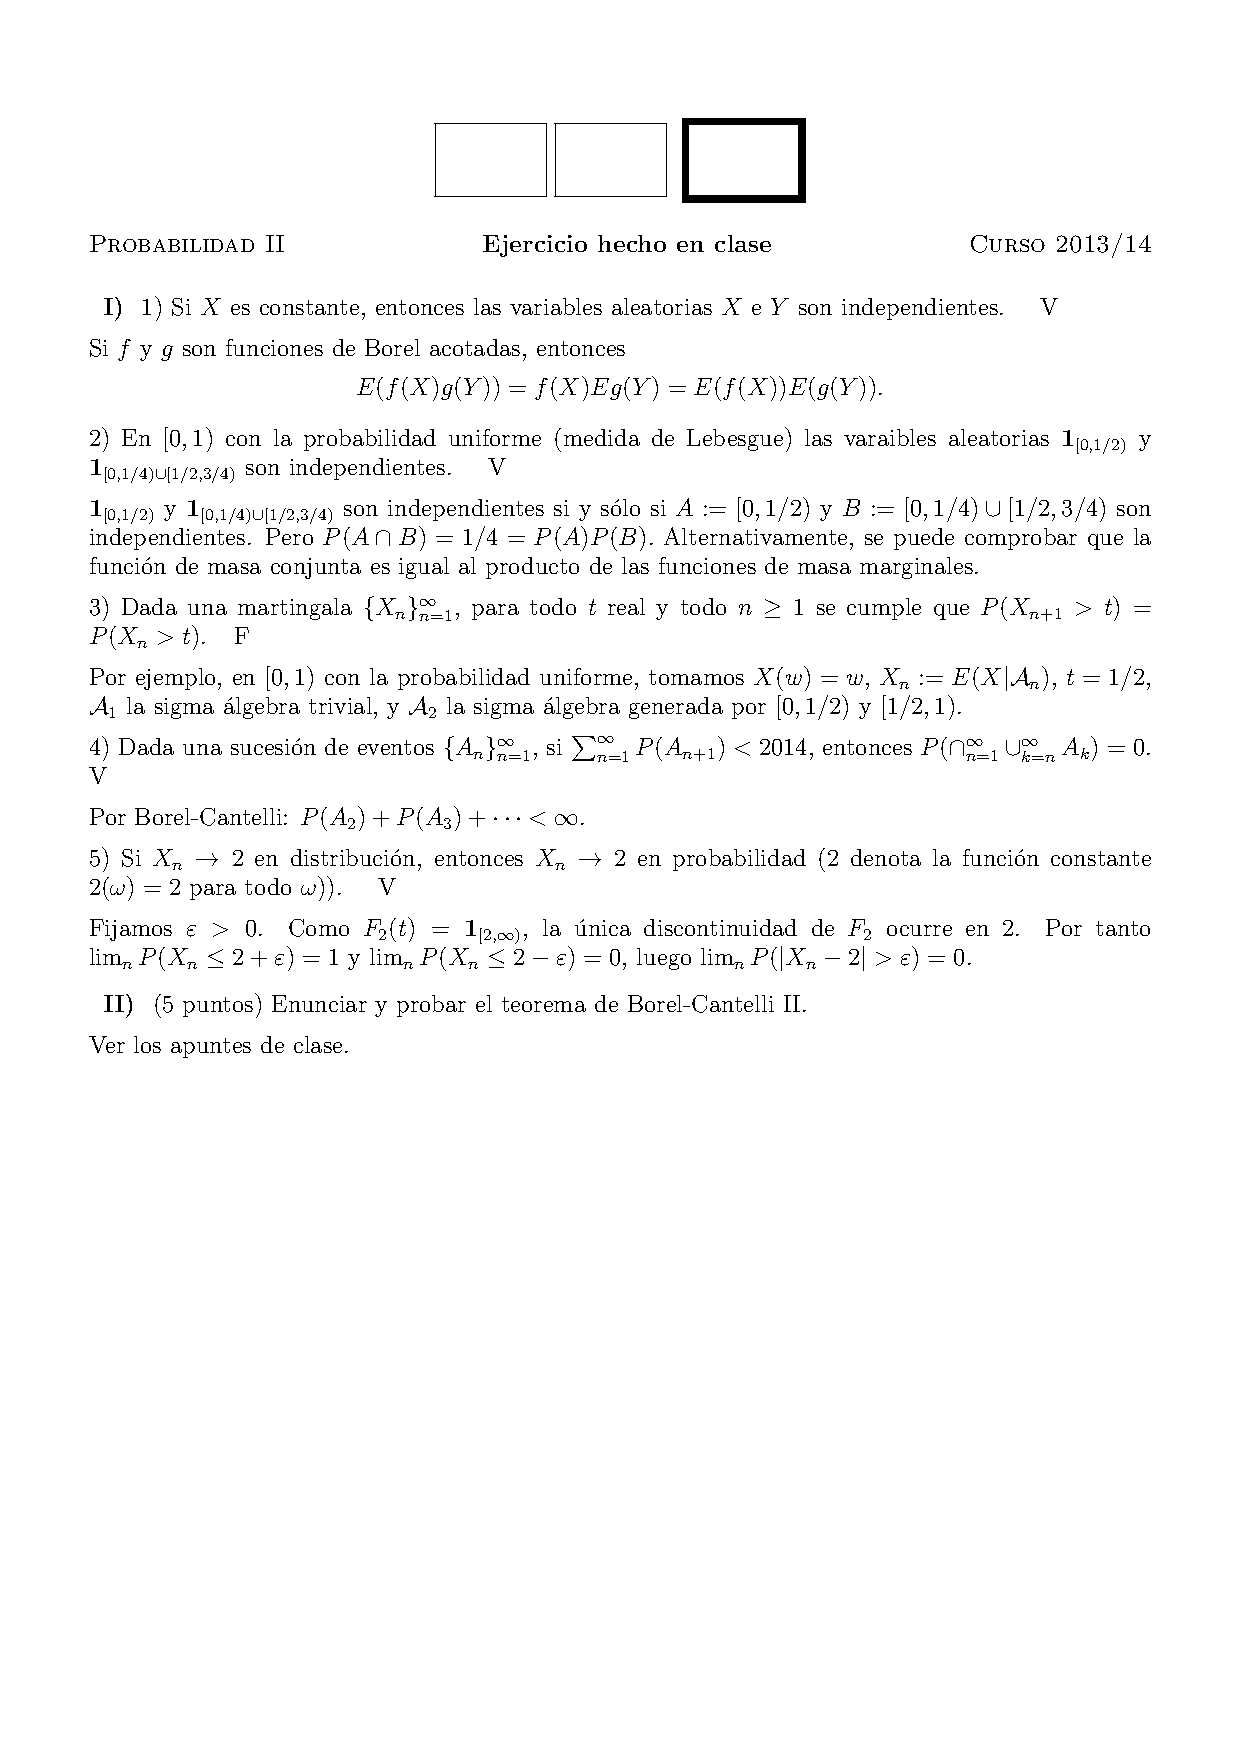
\includepdf[pages={1},scale=1]{pdf/_Probabilidad2Parcial2014soluciones.pdf}

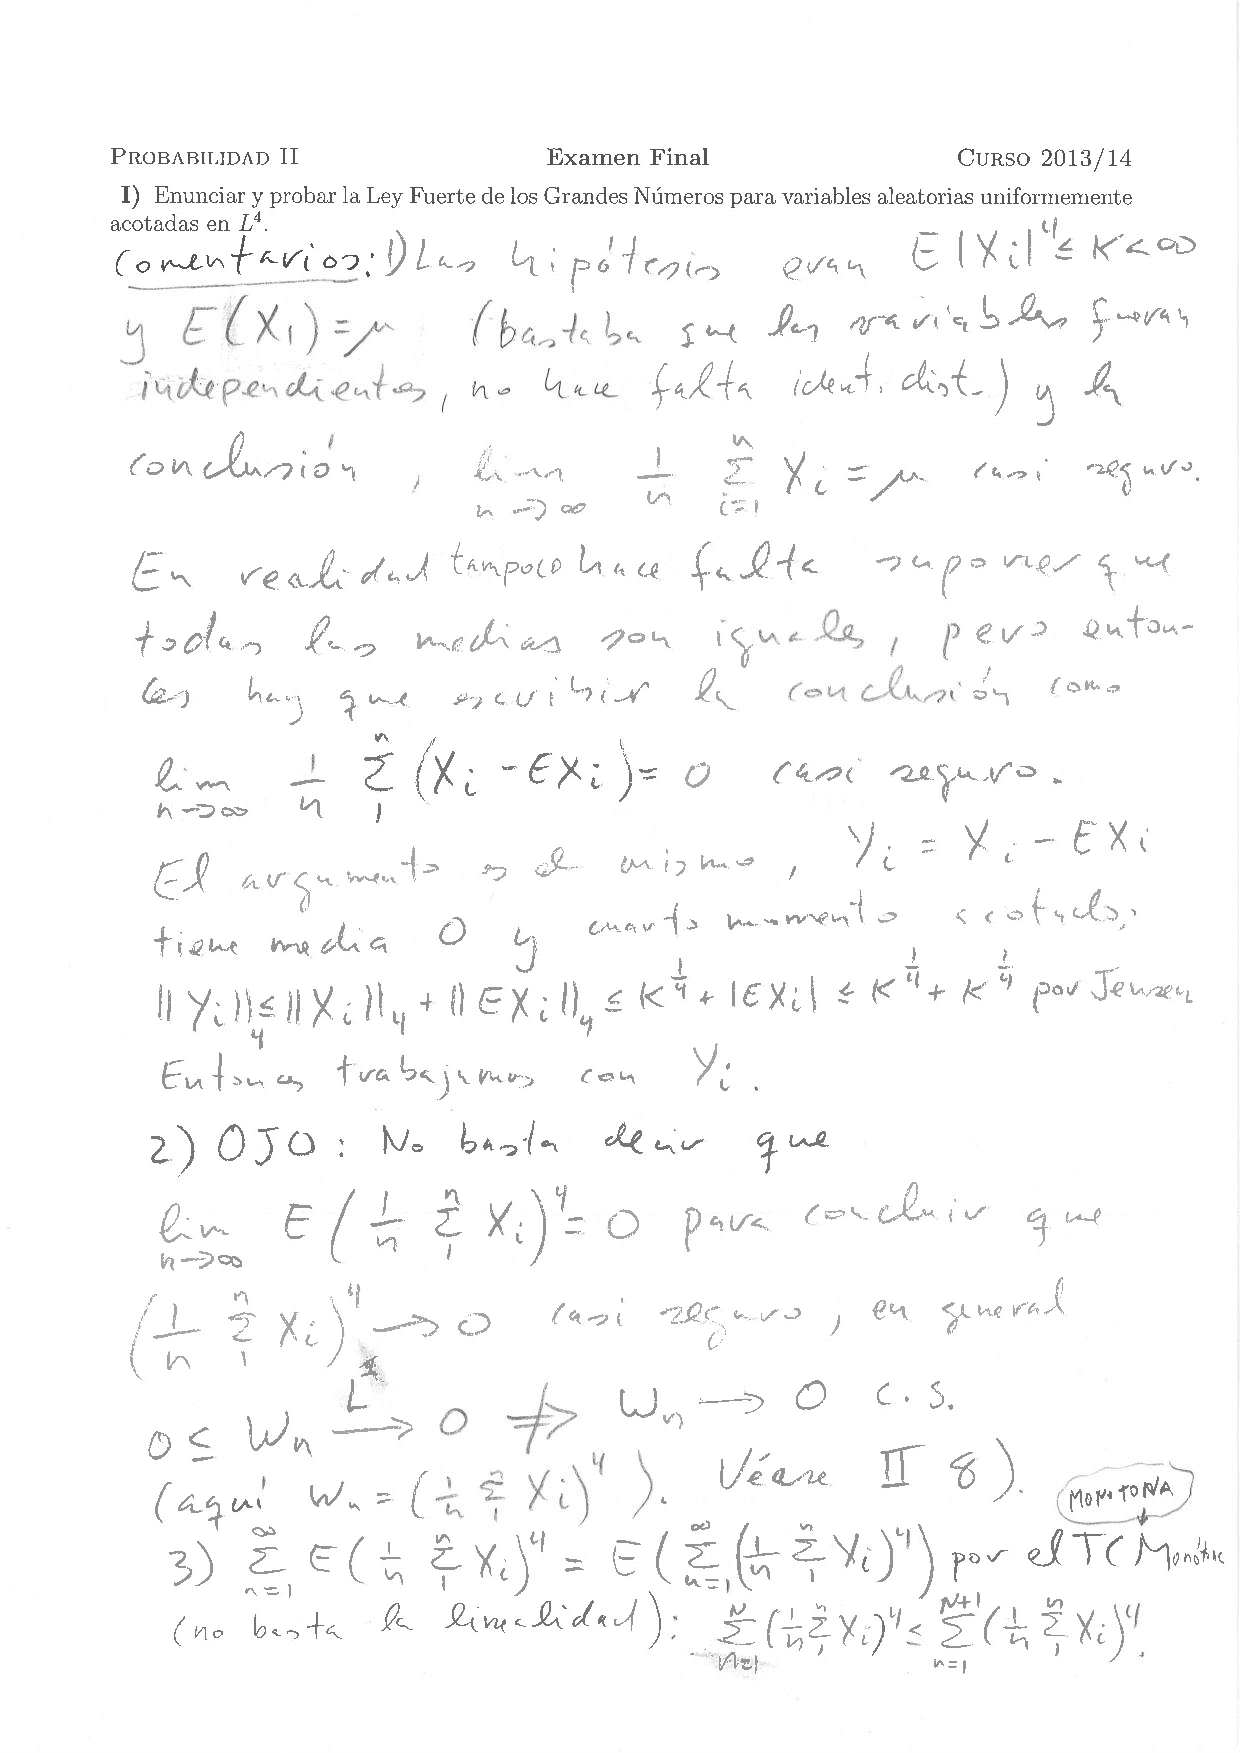
\includepdf[pages={1-8}, scale=1]{pdf/_SolnFinalMayo2014.pdf}



\end{document}

